\documentclass[a4paper, fontsize = 8pt, landscape]{scrartcl}
\usepackage{../../../misc_files/LateX/layout_and_colours}
\makeatletter
\def\input@path{{content/lecture_summary/}{content/examples/}}
\makeatother
\graphicspath{{content/images/}{content/lecture_summary/images/}{content/examples/images/}}

\title{Betriebssysteme}
\author{Jil Zerndt}
\date{FS 2025}

\createtitlepagestyle
\createmainpagestyle
\begin{document}
\begin{multicols}{2}
	\thispagestyle{TitlePageStyle}
	\maketitle
	\sffamily
	


\section{Overview of IT Security}

\mult{2}

\begin{definition}{Key IT Security Goals}
Information security is based on three fundamental principles, commonly known as the CIA triad:
\begin{itemize}
    \item \textbf{Confidentiality} - Ensuring data is only accessible to authorized users
    \item \textbf{Integrity} - Ensuring data is not modified in an unauthorized way
    \item \textbf{Availability} - Ensuring systems and data are accessible when needed
\end{itemize}
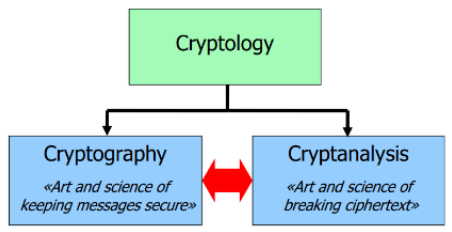
\includegraphics[width=0.6\linewidth]{its_goals.png}
\end{definition}

\begin{concept}{Business IT Risks}
\begin{itemize}
    \item Data loss
    \item System outage
    \item Espionage
    \item Sabotage
    \item Reputation loss
    \item Misuse of computing resources
    \item Violation of regulations
    \item Fraud
    \item Brand misuse
    \item Ransom demands
\end{itemize}
These risks can have significant financial, operational, and reputational impacts.
\end{concept}

\multend

\raggedcolumns

\subsubsection{Security Frameworks and Controls}

\mult{2}

\begin{concept}{Security Control Frameworks}
Security frameworks provide structured approaches to implementing security controls:
\begin{itemize}
    \item \textbf{CIS Controls} - Prioritized set of actions to protect organizations
    \item Controls are typically organized in implementation groups based on difficulty and impact
    \item Focus on preventing the most common attack vectors first
\end{itemize}
\end{concept}

\begin{definition}{Types of Security Measures}
Security measures can be categorized based on their focus:
\begin{itemize}
    \item \textbf{Preventive} - Block threats before they occur (firewalls, access controls)
    \item \textbf{Detective} - Identify when a breach has occurred (IDS, audit logs)
    \item \textbf{Corrective} - Mitigate damage after an incident (backups, incident response)
\end{itemize}
\end{definition}

\multend

\subsubsection{Disaster Recovery}



\begin{concept}{Business Continuity Management}
Disaster recovery and business continuity planning are essential for maintaining availability:
\begin{itemize}
    \item \textbf{Recovery Plan} - Detailed procedures for recovering from incidents
    \item \textbf{Recovery Tests} - Regular testing of recovery procedures
    \item \textbf{Redundancy} - Duplicate systems, power supplies, and network connections
    \item \textbf{Offline backups} - Protection against ransomware and other threats
\end{itemize}
\end{concept}

\begin{KR}{Disaster Recovery Planning}
\paragraph{Initial Assessment}
\begin{itemize}
    \item Identify critical systems and data
    \item Determine acceptable recovery time objectives (RTO)
    \item Determine acceptable recovery point objectives (RPO)
\end{itemize}

\paragraph{Plan Development}
\begin{itemize}
    \item Document recovery procedures
    \item Assign roles and responsibilities
    \item Include contact details for all relevant parties
    \item Develop technical instructions for restoration
\end{itemize}

\paragraph{Testing}
\begin{itemize}
    \item Conduct regular theoretical dry runs
    \item Perform practical tests (e.g., server shutdown, data restoration)
    \item Update procedures based on test results
\end{itemize}

\paragraph{Regular Review}
\begin{itemize}
    \item Review and update plans regularly
    \item Consider changes in infrastructure, personnel, and threats
\end{itemize}
\end{KR}

\begin{example}
A medium-sized company implements a disaster recovery plan for their customer database. They define an RTO of 4 hours and an RPO of 15 minutes, meaning they need to restore service within 4 hours with no more than 15 minutes of data loss. To achieve this, they implement a combination of hourly differential backups with continuous transaction log shipping to a standby site. Regular recovery tests are scheduled quarterly to ensure the plan remains effective.
\end{example}

\mult{2}


\begin{concept}{Problems - Overview}\\ and their impact on data availability
\paragraph{Physisch}
\textbf{unabsichtlich}
\begin{itemize}
    \item Naturkatastrophen
    \item Feuer
    \item Ausfall
    \item Kaffee auf Server
\end{itemize}

\textbf{absichtlich/bösartig}
\begin{itemize}
    \item Feuer
    \item Vandalismus
    \item Garantie läuft aus -> absichtlich langsamer
    \item Social Engineering
\end{itemize}

\paragraph{Virtuell}
\textbf{unabsichtlich}
\begin{itemize}
    \item Bitflip
    \item Config Fehler
    \item Bugs im SW
    \item Phishing klicken
\end{itemize}

\textbf{absichtlich/bösartig}
\begin{itemize}
    \item DDoS
    \item Malware
    \item Ransomware
    \item Phishing senden
    \item Trojaner
\end{itemize}
\end{concept}

\begin{theorem}{Countermeasures - Overview}

\textbf{Disaster Recovery}
    \begin{itemize}
        \item Offline backup solutions
        \item Restoring from images
    \end{itemize}

\textbf{Access Control}
    \begin{itemize}
        \item Restricted Access Rights
        \item Multi-Factor Authentication
        \item Firewalls
        \item Traffic Management Solutions
    \end{itemize}

\textbf{Physical Protection}
    \begin{itemize}
        \item Physical Access Control (locks, fences, etc.)
        \item Fire Protection (extinguishers, alarms, etc.)
        \item Monitoring (CCTV, Guards etc.)
    \end{itemize}

\textbf{Training Processes}
    \begin{itemize}
        \item Employee Training
        \item Four eyes principle
        \item Automation of routine processes
        \item Monitoring
        \item Preventive maintenance
    \end{itemize}

\textbf{Redundancy}
    \begin{itemize}
        \item Uninterruptable Power Supplies
        \item High Availability setups
        \item Load Balancing
        \item Redundant data center
        \item Redundant network connections
    \end{itemize}
\end{theorem}

\multend

\mult{2}

\begin{formula}{Recovery Plan and Test}

    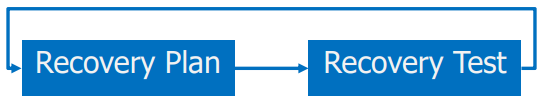
\includegraphics[width=0.7\linewidth]{recovery_plan_test.png}

    \textbf{Recovery Plan} - description of what to do if something goes wrong
    \begin{itemize}
        \item Roles and responsibilities
        \item Processes
        \item Contact details
        \item Technical instructions
    \end{itemize}

    \textbf{Recovery Test} - testing the recovery plan
    \begin{itemize}
        \item Theoretical dry run
        \item Practical tests
        \begin{itemize}
            \item turn off a server or DC
            \item restore data from backup
        \end{itemize}
    \end{itemize}
\end{formula}

\begin{concept}{Goals of IT Security}

Most measures in Information Security have one of the three following high-level goals:
\begin{itemize}
    \item Ensure data is confidential
    \item Ensure data is not corrupted
    \item Ensure data and systems are available
\end{itemize}

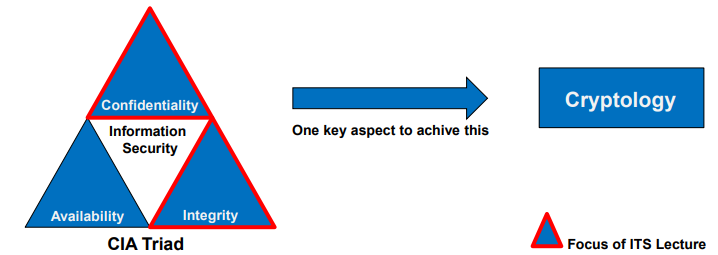
\includegraphics[width=\linewidth]{goals_of_IT_security.png}
\end{concept}

\multend

\raggedcolumns





	\raggedcolumns
	\pagebreak
	\section{Linux Primer}

\subsection{Terminal Basics}

\mult{2}

\begin{definition}{Terminal}\\
    A terminal is a text-based user interface program that allows users to:
    \begin{itemize}
        \item Accepts text input via a prompt
        \item Interprets text as commands
        \item Executes operations based on user input
        \item Returns output to the user
    \end{itemize}
    \vspace{2mm}
    Terminal commands can be:
    \begin{itemize}
        \item Binary programs loaded from disk (e.g., \texttt{mkdir})
        \item Built-in functions of the terminal (e.g., \texttt{cd})
        \item Operations like regular expressions for complex command preparation
    \end{itemize}
\end{definition}

\begin{KR}{Essential Terminal Commands}
    \paragraph{System information}
    \begin{itemize}
        \item \texttt{whoami} - Display current user
        \item \texttt{uname -a} - Display kernel information
        \item \texttt{lsmod} - List loaded kernel modules
        \item \texttt{dmesg} - Display kernel messages
    \end{itemize}
    
    \paragraph{Command output manipulation}
    \begin{itemize}
        \item \texttt{command > file.txt} - Redirect output to a file
        \item \texttt{command | grep pattern} \\ - Filter output through grep
        \item \texttt{clear} - Clear terminal screen
    \end{itemize}
    
    \paragraph{System control}
    \begin{itemize}
        \item \texttt{env} - Display environment variables
        \item \texttt{exit} - Exit the terminal
        \item \texttt{shutdown} - Shutdown the system
    \end{itemize}
\end{KR}

\multend

\mult{2}

\subsection{User Management}

\begin{definition}{User Management in Linux} Tools:
    \begin{itemize}
        \item \texttt{users} - List users currently logged in
        \item \texttt{who} - Show who is logged in
        \item \texttt{id} - Display user and group IDs
        \item \texttt{passwd} - Change user password
        \item \texttt{usermod} - Modify user account
        \item \texttt{groupmod} - Modify a group
    \end{itemize}
    
    Administrative access:
    \begin{itemize}
        \item \texttt{root} - Account with full system privileges
        \item \texttt{sudo} - Execute command as root user
        \item \texttt{su} - Switch user
        \item \texttt{su -} - Switch user and load their environment
    \end{itemize}
\end{definition}

\subsection{Process Management}

\begin{definition}{Process Management Commands}\\
    Commands for monitoring and controlling processes:
    \begin{itemize}
        \item \texttt{ps} - Display current processes
        \item \texttt{top} - Interactive process viewer
        \item \texttt{pstree} - Display process tree
        \item \texttt{pidof} - Find process ID of a program
        \item \texttt{kill} - Send signal to process
        \item \texttt{kill -9} - Force terminate process
        \item \texttt{killall} - Kill processes by name
    \end{itemize}
\end{definition}

\multend

\subsection{Files, Directories, and Filesystems}

\mult{2}

\begin{definition}{File System Operations}\\
    Basic file and directory operations:
    \begin{itemize}
        \item \texttt{pwd} - Print working directory
        \item \texttt{cd} - Change directory
        \item \texttt{ls -al} - List all files with details
        \item \texttt{touch} - Create empty file or update timestamp
        \item \texttt{mkdir} - Create directory
        \item \texttt{tree} - Display directory structure as a tree
        \item \texttt{cp} - Copy files/directories
        \item \texttt{mv} - Move/rename files/directories
        \item \texttt{rm} - Remove files/directories
    \end{itemize}
    
    File permissions and ownership:
    \begin{itemize}
        \item \texttt{chown} - Change file owner
        \item \texttt{chmod} - Change file permissions
    \end{itemize}
    
    Disk and filesystem management:
    \begin{itemize}
        \item \texttt{fdisk -l} - List disk partitions
        \item \texttt{mount} - Mount a filesystem
    \end{itemize}
\end{definition}

\begin{KR}{Working with Files in Linux}
    \paragraph{Creating and viewing files}
    \begin{itemize}
        \item \texttt{touch filename} - Create empty file
        \item \texttt{cat filename} - Display entire file contents
        \item \texttt{less filename} - View file with pagination
        \item \texttt{tail filename} - Display last 10 lines of file
        \item \texttt{tail -f filename} - Continuously monitor file for changes
    \end{itemize}
    
    \paragraph{Text editing with vim}
    \begin{itemize}
        \item \texttt{vim filename} - Open file in vim
        \item Press \texttt{i} for insert mode
        \item Press \texttt{Esc} to exit insert mode
        \item Type \texttt{:w} to save
        \item Type \texttt{:q} to quit
        \item Type \texttt{:wq} to save and quit
        \item Type \texttt{:q!} to quit without saving
    \end{itemize}
\end{KR}

\multend

\subsection{System Information and Configuration}

\mult{2}

\begin{definition}{System Information Commands}\\
    Commands for system information/configuration:
    \begin{itemize}
        \item \texttt{hwinfo} - Hardware information
        \item \texttt{lshw} - List hardware
        \item \texttt{/proc} - Virtual filesystem for kernel information
        \item \texttt{/etc} - Configuration files directory
        \item \texttt{sysctl} - Read/modify kernel parameters
        \item \texttt{systemctl} - Control the systemd system and service manager
    \end{itemize}
    
    Network-related commands:
    \begin{itemize}
        \item \texttt{ifconfig} - Configure network interfaces
        \item \texttt{ip} - Show/manipulate routing, devices, policy routing
        \item \texttt{dig} - DNS lookup utility
        \item \texttt{hostname} - Show or set system hostname
    \end{itemize}
    
    Package management:
    \begin{itemize}
        \item \texttt{apt-get} - Package handling utility
    \end{itemize}
\end{definition}

\begin{example2}
    {Working with the Linux terminal}
    
    \begin{lstlisting}[language=bash, style=basesmol]
    # Check current user
    whoami
    
    # View hardware information
    lshw -short
    
    # Monitor system messages
    dmesg | grep usb
    
    # Check disk usage
    df -h
    
    # Find a process ID
    pidof firefox
    
    # Install a package
    sudo apt-get install htop
    \end{lstlisting}
\end{example2}

\begin{KR}{OpenStack Lab Environment Setup}
    \paragraph{Initial setup}
    \begin{itemize}
        \item Connect to ZHAW VPN if not at ZHAW facilities
        \item Navigate to OpenStack Horizon dashboard: \texttt{https://ned.cloudlab.zhaw.ch}
        \item Log in with provided credentials
        \item Change password if using default credentials
    \end{itemize}
    
    \paragraph{Creating SSH key pair}
    \begin{itemize}
        \item Go to Compute $\rightarrow$ Key Pairs $\rightarrow$ Create Key Pair
        \item Download the private key file (*.pem)
        \item Set appropriate permissions: \\ \texttt{chmod 600 key.pem}
    \end{itemize}
    
    \paragraph{Creating a VM}
    \begin{itemize}
        \item Go to Compute $\rightarrow$ Instances $\rightarrow$ Launch Instance
        \item Select Ubuntu image
        \item Attach to 'internal' network
        \item Set SSH key and security groups
        \item Launch VM and associate a Floating IP
    \end{itemize}
    
    \paragraph{Connecting to VM}
    \begin{itemize}
        \item SSH to the VM: \\ \texttt{ssh -i key.pem ubuntu@IP\_ADDRESS}
    \end{itemize}
\end{KR}

\begin{example2}{Linux Lab Basic Tasks}
    Creating/managing files:
    \begin{lstlisting}[language=bash, style=basesmol]
    # Create a test file
    touch delta.txt
    # Add content to the file
    echo "Hello, this is a test" > delta.txt
    # View the file content
    cat delta.txt
    # Stop and restart the VM from OpenStack dashboard
    # Then check if the file persists
    cat delta.txt
    \end{lstlisting}
\end{example2}

\multend
	\raggedcolumns
	\pagebreak
	\section{Booting an OS}

\subsection{Boot Process and Initialization}



\begin{formula}{Boot Process Stages}
    Typical boot process follows these steps:
    \begin{itemize}
        \item Hardware initialization (BIOS/UEFI)
        \item Bootloader execution
        \item Kernel loading and initialization
        \item System initialization (services, environment)
        \item User interface presentation
    \end{itemize}
\end{formula}

\mult{2}

\subsubsection{BIOS and Bootloader}

\begin{concept}{BIOS and Hardware Initialization }\\
    BIOS (Basic Input Output System) is the first program loaded on boot:
    \begin{itemize}
        \item Stored in ROM on the motherboard
        \item Contains low-level I/O software for interfacing with devices
        \item Performs Power-On Self-Test (POST)
        \item Discovers devices by scanning PCI buses
        \item Initializes hardware devices
        \item Selects a boot device from the list in CMOS
        \item Reads the first sector from the boot device (Master Boot Record)
        \item Loads MBR into memory and executes it
    \end{itemize}
\end{concept}

\begin{definition}{Bootloader Function}\\
    The bootloader (loaded from MBR):
    \begin{itemize}
        \item Accesses the boot partition containing the OS
        \item Loads the OS kernel into memory
        \item Sets up registers (Program Counter, Processor Status Word)
        \item Transfers control to the OS by jumping to the first instruction
    \end{itemize}
\end{definition}

\begin{definition}{GRUB (GRand Unified Bootloader)}\\
    GRUB is a common bootloader for Linux systems:
    \begin{itemize}
        \item Requires filesystem access to read the OS
        \item Contains device drivers and filesystem modules
        \item Provides a menu to select the OS to boot
        \item Loads the selected kernel and optional initial RAM disk (initrd)
        \item Passes control to the kernel
    \end{itemize}
\end{definition}

\multend

\paragraph{BIOS vs UEFI}

\mult{2}

\begin{definition}{BIOS Limitations}\\
    Traditional BIOS has several limitations:
    \begin{itemize}
        \item Operates in 16-bit mode
        \item Relies on MBR (Master Boot Record) from 1983
        \item Limited partition number and size (2 TB max)
        \item Not designed for extendability
        \item Vulnerable to rootkit and bootkit attacks
    \end{itemize}
\end{definition}

\begin{definition}{Unified Extensible Firmware Interface (UEFI)}\\
    UEFI is the modern replacement for BIOS:
    \begin{itemize}
        \item Replaces MBR with GPT (GUID Partitioning Table)
        \item Supports arbitrary number of partitions
        \item Addresses disk space up to 2\textsuperscript{64} bytes
        \item Uses unique UUIDs for partitions to avoid collisions
        \item Features modular design for extendability
        \item Includes "Secure Boot" to restrict which binaries can be executed
        \item Uses cryptographic signatures and X.509 certificates for verification
    \end{itemize}
\end{definition}

\begin{definition}{UEFI Functioning}\\
    UEFI uses an architecture-independent virtual machine:
    \begin{itemize}
        \item Executes special binary files compiled for UEFI (*.efi)
        \item These files can be device drivers, bootloaders, or extensions
        \item Files are stored in the EFI System Partition (ESP)
        \item ESP uses FAT filesystem and can be reused in multi-boot systems
        \item EFI Boot Manager configures which EFI binary to execute
    \end{itemize}
\end{definition}

\begin{example}
    Examining UEFI boot configuration:
    \begin{lstlisting}[language=bash, style=basesmol]
    # Display current boot entries
    sudo efibootmgr -v
    
    # List contents of EFI system partition
    sudo ls -la /boot/efi/EFI/
    
    # View disk partition table format (MBR or GPT)
    sudo fdisk -l
    \end{lstlisting}
\end{example}

\multend

\subsubsection{OS Kernel Initialization}

\mult{2}

\begin{concept}{Kernel Initialization}\\
    The OS kernel initialization process:
    \begin{itemize}
        \item Queries hardware information 
        \item Loads and initializes device drivers
        \item Initializes internal management structures \\ (e.g., process table)
        \item Sets up virtual memory and \\ memory management
        \item Creates system services
        \item Launches the first user process (init)
    \end{itemize}
\end{concept}

\begin{theorem}{Linux Kernel Initialization Phases}
    \begin{itemize}
        \item Architecture-specific assembly code
            \begin{itemize}
                \item Sets up OS memory map
                \item Identifies CPU type
                \item Calculates total RAM
                \item Disables interrupts
                \item Enables MMU and caches
            \end{itemize}
        \item C main() procedure
            \begin{itemize}
                \item Initializes process tables, \\ interrupt/system-call tables
                \item Sets up virtual memory and page cache
                \item Configures resource control
                \item Loads drivers and initializes OS services
            \end{itemize}
    \end{itemize}
\end{theorem}

\multend

\subsubsection{Initial RAM Disk (initrd/initramfs)}

\begin{definition}{Initial RAM Disk}\\
    The initial RAM disk addresses the "chicken-and-egg" problem:
    \begin{itemize}
        \item OS needs drivers to access hard drive and its filesystem
        \item These drivers are stored on the hard drive itself
        \item Solution: initrd/initramfs provides temporary root filesystem
        \item Contains kernel modules and basic device files
        \item Bootloader uncompresses both kernel and initrd into RAM
        \item Kernel mounts initrd as the initial filesystem
        \item Kernel uses tools found in initrd to find and mount the real filesystem
    \end{itemize}
\end{definition}

\begin{example}
    Examining GRUB configuration for kernel and initrd:
    \begin{lstlisting}[language=bash, style=basesmol]
    # View GRUB configuration
    cat /boot/grub/grub.cfg
    
    # Examine a specific menu entry showing kernel and initrd paths
    grep -A 10 "menuentry 'Ubuntu'" /boot/grub/grub.cfg
    \end{lstlisting}
\end{example}

\subsubsection{System Services Initialization}



\begin{concept}{System V Init}\\
    Traditional System V initialization:
    \begin{itemize}
        \item Init process runs initialization shell scripts from /etc/rc\# directories
        \item Uses predefined runlevels (0-6) to determine system state
        \item Each runlevel has a set of services defined in scripts
        \item Dependencies among services are coded in the scripts themselves
        \item Results in complex initialization process
    \end{itemize}
    \vspace{2mm}
    System V runlevels:
    \begin{itemize}
        \item 0: Halt - Shuts down the system
        \item 1: Single-user mode - Administrative tasks
        \item 2: Multi-user mode without networking
        \item 3: Multi-user mode with networking
        \item 4: Not used/user-definable
        \item 5: Multi-user mode with GUI
        \item 6: Reboot - Restarts the system
    \end{itemize}
\end{concept}

\subsubsection{systemd}

\mult{2}

\begin{definition}{systemd}\\
    Modern initialization system (systemd):
    \begin{itemize}
        \item Replacement for SysV Init
        \item Provides coordinated and parallel service startup
        \item Features on-demand activation and \\ runtime management
        \item Uses dependency-based service control logic
        \item Takes a holistic management approach for \\ the entire system
    \end{itemize}
\end{definition}

\begin{definition}{systemd User Services}\\
    systemd supports user instance services:
    \begin{itemize}
        \item Services managed by individual users \\ without requiring root privileges
        \item User service units are stored in:
            \begin{itemize}
                \item Units provided by packages: \\ \texttt{/usr/lib/systemd/user/}
                \item User-installed package units: \\ \texttt{\textasciitilde/.local/share/systemd/user/}
                \item System-wide user units: \\ \texttt{/etc/systemd/user/}
                \item User's own units: \\ \texttt{\textasciitilde/.config/systemd/user/}
            \end{itemize}
        \item By default, user services start on login \\ and stop on logout
        \item Lingering allows user services to \\ start at boot without login
    \end{itemize}
\end{definition}

\begin{definition}{systemd Dependencies}\\
    systemd supports various dependency types:
    \begin{itemize}
        \item \textbf{Requires=} \\ Units that must be started when this \\ unit is started
        \item \textbf{Wants=} \\ Units that should be started (but not required) when this unit is started
        \item \textbf{Conflicts=} \\ Units that must be stopped when this unit is started
        \item \textbf{After=} \\ This unit should be started after the listed units
        \item \textbf{Before=} \\ This unit should be started before the listed units
    \end{itemize}
\end{definition}

\begin{definition}{systemd Units}\\
    systemd organizes system components as 'units' which:
    \begin{itemize}
        \item encapsulate system objects \\ (services, mounts, devices, etc.)
        \item have states \\ (active, inactive, activating, deactivating, failed)
        \item can depend on other units
        \item (most) are configured in unit configuration files
        \item (some) can be created automatically \\ or programmatically
    \end{itemize}
    \vspace{2mm}
    \textbf{Common unit types:}
    \begin{itemize}
        \item .service - A system service
        \item .target - A group of systemd units \\ (similar to runlevels)
        \item .mount - A filesystem mount point
        \item .device - A device file recognized by the kernel
        \item .socket - An inter-process communication socket
        \item .timer - A systemd timer
    \end{itemize}
\end{definition}

\begin{code}{systemd Service Unit File}\\
    A systemd service unit file consists of three sections:
    
\begin{lstlisting}[language=bash, style=basesmol]
[Unit]
Description=Example Service
Documentation=https://example.com/docs
After=network.target
Wants=network-online.target
Requires=example-dependency.service

[Service]
Type=simple
ExecStart=/usr/bin/example-service
Restart=on-failure
User=exampleuser

[Install]
WantedBy=multi-user.target
\end{lstlisting}

    The sections have specific purposes:
    \begin{itemize}
        \item Unit: Metadata and dependencies
        \item Service: Execution configuration for services
        \item Install: Configuration for enabling the unit
    \end{itemize}
\end{code}

\multend

\begin{KR}{Working with systemd}
    \paragraph{Viewing unit status}
    \begin{itemize}
        \item \texttt{systemctl status -all} - Show status of all units
        \item \texttt{systemctl status SERVICE} - Show status of specific service
        \item \texttt{systemctl list-units -t service} - List only service units
        \item \texttt{systemctl list-unit-files --type service} - List service unit files
        \item \texttt{systemctl cat SERVICE} - View the content of a unit file
    \end{itemize}
    
    \paragraph{Managing units}
    \begin{itemize}
        \item \texttt{systemctl start SERVICE} - Start a service
        \item \texttt{systemctl stop SERVICE} - Stop a service
        \item \texttt{systemctl restart SERVICE} - Restart a service
        \item \texttt{systemctl enable SERVICE} - Enable service autostart
        \item \texttt{systemctl disable SERVICE} - Disable service autostart
    \end{itemize}
    
    \paragraph{Working with targets}
    \begin{itemize}
        \item \texttt{systemctl list-units -t target} - List available targets
        \item \texttt{systemctl get-default} - Show default target
        \item \texttt{systemctl set-default TARGET} - Set default target
    \end{itemize}
\end{KR}

\begin{example2}{Creating a Simple systemd Service}\\
    Creating a custom service to write to a file when started:
    
\begin{lstlisting}[language=bash, style=basesmol]
# Create a service unit file
sudo nano /etc/systemd/system/myservice.service

# Add the following content
[Unit]
Description=My Simple Service
After=network.target

[Service]
Type=simple
ExecStart=/bin/bash -c 'echo "Service started at $(date)" > /home/ubuntu/service_started'
Restart=on-failure

[Install]
WantedBy=multi-user.target

# Reload systemd to recognize the new service
sudo systemctl daemon-reload

# Start the service
sudo systemctl start myservice

# Verify it worked
cat /home/ubuntu/service_started

# Enable auto-start on boot
sudo systemctl enable myservice
\end{lstlisting}
\end{example2}




	\raggedcolumns
	\pagebreak
	\section{Processes and Threads}

\subsection{Processes}

\subsubsection{Process Model}

\begin{definition}{Programs vs. Processes}
    A program is fundamentally different from a process:
    \vspace{1mm}\\
    \begin{minipage}{0.5\linewidth}
    \textbf{Program}: A compiled executable (binary)
            \begin{itemize}
                \item Set of CPU instructions and related data
                \item Targets a specific platform (OS + hardware)
                \item Static entity stored on disk
            \end{itemize}
        \end{minipage}
    \begin{minipage}{0.5\linewidth}
        \textbf{Process}: An active instance of a program
            \begin{itemize}
                \item Has a program, input, output, and state
                \item Dynamic entity in memory
                \item Multiple instances of the same program can run as separate processes
            \end{itemize}
    \end{minipage}
\end{definition}

\mult{2}

\begin{definition}{Process Characteristics}\\
    Processes have several important characteristics:
    \begin{itemize}
        \item Can run sequentially or in parallel (multi-tasking)
        \item Selected for execution by the OS scheduler
        \item Associated with an owner \\ (defines access privileges)
        \item Run within an environment \\ (environment variables)
        \item Can run in foreground (interactive) \\ or background (non-interactive)
        \item Can be user processes or system processes
    \end{itemize}
\end{definition}

\begin{example2}{Viewing process information in Linux}
\begin{lstlisting}[language=bash, style=basesmol]
# List all processes with details
ps aux
# Interactive process viewer
top
# Show environment variables
env
# Run a process in the background
wc /dev/zero &
# List background jobs
jobs
# Bring a background job to foreground
fg %job_number
\end{lstlisting}
\end{example2}

\multend

\subsubsection{Process Creation}

\mult{2}

\begin{definition}{Process Creation by the OS}\\
    When creating a process, the OS performs several operations:
    \begin{itemize}
        \item Loads the executable into RAM
        \item Sets up the memory map
        \item Updates scheduler and process table entries
        \item Sets program counter and stack pointer
        \item Switches from system mode to user mode
    \end{itemize}
\end{definition}

\begin{definition}{Memory Layout}\\
    Process memory is typically divided into several segments:
    \begin{itemize}
        \item \textbf{Text}: Contains CPU instructions and constant data
        \item \textbf{Data}: Global and static variables
            \begin{itemize}
                \item Initialized data segment: Pre-initialized variables
                \item Uninitialized data segment (BSS): Zero-initialized variables
            \end{itemize}
        \item \textbf{Stack}: Local variables and function call information (LIFO structure)
        \item \textbf{Heap}: Dynamically allocated memory (controlled by the programmer)
    \end{itemize}
\end{definition}

\begin{definition}{Process Creation Events}\\
    Processes can be created in several ways:
    \begin{itemize}
        \item System boot (initial processes)
        \item User request (launching an application)
        \item Process creating another process (fork/exec)
        \item Scheduled creation (cron jobs)
        \item System request (responding to interrupts)
    \end{itemize}
\end{definition}

\begin{definition}{Parent-Child Process Relationship}\\
    When a process creates another process:
    \begin{itemize}
        \item The creating process becomes the parent
        \item The new process becomes the child
        \item Child's memory map is initially a copy of the parent's memory map
        \item Two memory handling approaches:
            \begin{itemize}
                \item Distinct address space: Separate memory regions for parent and child
                \item Copy-on-write: Memory shared until a change is made by either process
            \end{itemize}
        \item Forms a process hierarchy (starting with PID 1)
    \end{itemize}
\end{definition}

\begin{example2}{Linux Process Creation}\\
    Linux terminal command execution involves process creation:
\begin{lstlisting}[language=bash, style=basesmol]
# When you run a command in the terminal:
ls -la

# The shell:
# 1. Forks itself (duplicate the process)
# 2. Child process executes the 'ls' binary
# 3. Parent waits for child to complete
# 4. Shell continues after child terminates
\end{lstlisting}

    This process can be visualized with \texttt{pstree} showing the parent-child relationships.
\end{example2}

\multend

\subsubsection{Process Termination}

\mult{2}

\begin{definition}{Process Termination}\\
    A process can terminate in several ways:
    \begin{itemize}
        \item Voluntary normal exit (job completed, return from main())
        \item Voluntary error exit (required resource unavailable)
        \item Involuntary error exit (segmentation fault, division by zero)
        \item Termination by another process (kill signal)
    \end{itemize}
\end{definition}

\begin{example}
    Process termination in Linux:
    \begin{lstlisting}[language=bash, style=basesmol]
    # Start a process
    wc /dev/zero &
    
    # Get its process ID
    pidof wc
    
    # Terminate the process
    kill -9 <PID>
    \end{lstlisting}
\end{example}

\multend

\subsubsection{Process States}

\mult{2}

\begin{definition}{Process States}\\
    Each process has a life-cycle with specific states:
    \begin{itemize}
        \item \textbf{Running}: The process is currently executing on the CPU
        \item \textbf{Ready}: The process is ready to run but waiting for CPU allocation
        \item \textbf{Blocked}: The process is unable to run (waiting for an event or resource)
            \begin{itemize}
                \item Dependencies not met for running
                \item Waiting for external resource
                \item Waiting for I/O completion
                \item Sleeping
                \item Under job control or debugger
            \end{itemize}
    \end{itemize}
\end{definition}



\begin{concept}{User Mode vs. System Mode}\\
    CPU supports two execution modes:
    \begin{itemize}
        \item \textbf{User Mode}: Limited privileges
            \begin{itemize}
                \item Application logic execution
                \item Application data manipulation
                \item Restricted access to hardware and system resources
            \end{itemize}
        \item \textbf{System Mode} (Kernel Mode): Full privileges
            \begin{itemize}
                \item System management operations
                \item Hardware access
                \item Interrupt handling
                \item Device management
            \end{itemize}
    \end{itemize}
\end{concept}

\begin{definition}{Process State Changes}\\
    Processes change state for various reasons:
    \begin{itemize}
        \item \textbf{Timer expiration}: CPU allocation time ended
        \item \textbf{Interrupt}: Hardware/resource calls for service
        \item \textbf{Page fault}: Data not in memory, requires disk access
        \item \textbf{System call}: Explicit OS service request
    \end{itemize}
    
    State changes involve a switch between user mode and system (kernel) mode.
\end{definition}

\begin{concept}{Context Switch vs. Mode Switch}\\
    Two types of switches occur during system operation:
    \begin{itemize}
        \item \textbf{Mode Switch}: Transition between user mode and kernel mode
            \begin{itemize}
                \item Occurs during system calls, interrupts, exceptions
                \item Same process continues execution in different mode
                \item No scheduler involvement
            \end{itemize}
        \item \textbf{Context Switch}: Changing from one process to another
            \begin{itemize}
                \item Involves saving the state of the current process
                \item Loading the state of another process
                \item Typically involves mode switches (user $\rightarrow$ kernel $\rightarrow$ user)
                \item Requires scheduler involvement
            \end{itemize}
    \end{itemize}
\end{concept}

\multend

\raggedcolumns
\columnbreak

\subsubsection{Process Management}

\begin{definition}{Process Control Block}\\
    The OS maintains a Process Control Block (PCB) for each process:
    \begin{itemize}
        \item Process identification (PID, UID, GID)
        \item Process state information
        \item Program counter and CPU registers
        \item CPU scheduling information (priority)
        \item Memory management information
        \item I/O status information
        \item Accounting information
    \end{itemize}
    
    In Linux, PCBs are implemented as \texttt{task\_struct} entries in the process table.
\end{definition}

\begin{KR}{Process Management in Linux}
    \paragraph{Viewing process information}
    \begin{itemize}
        \item \texttt{ps aux} - List all processes
        \item \texttt{ps -ef} - List processes in full format
        \item \texttt{ps -eLF} - List processes and threads
        \item \texttt{top} - Interactive process viewer
        \item \texttt{top -H} - Show threads in top
        \item \texttt{pstree} - Display process tree
    \end{itemize}
    
    \paragraph{Creating processes}
    \begin{itemize}
        \item Write a C program using \texttt{fork()} to create a child process
        \item Use \texttt{getpid()} to retrieve the process ID
        \item Use \texttt{sleep()} to pause execution
    \end{itemize}
    
    \paragraph{Identifying zombie processes}
    \begin{itemize}
        \item Create a parent process that doesn't wait for its child
        \item Child terminates while parent continues running
        \item Check process state with \texttt{ps} (state "Z" indicates zombie)
    \end{itemize}
\end{KR}

\begin{example2}{Creating Processes in C}\\
    Simple process creation with fork():
    
\begin{lstlisting}[language=C, style=basesmol]
#include <stdio.h>
#include <stdlib.h>
#include <unistd.h>

int main() {
    pid_t pid = fork();
    
    if (pid < 0) {
        // Error
        fprintf(stderr, "Fork failed\n");
        return 1;
    } else if (pid == 0) {
        // Child process
        printf("Child process: PID = %d\n", getpid());
        sleep(5);
    } else {
        // Parent process
        printf("Parent process: PID = %d, Child PID = %d\n", getpid(), pid);
        sleep(10);
    }
    
    return 0;
}
\end{lstlisting}
\end{example2}

\subsubsection{Fork Process Trees}

\begin{KR}{Fork() Process Tree Analysis}
    \paragraph{Understanding fork() behavior}
    \begin{itemize}
        \item fork() creates an exact copy of the calling process
        \item Returns child PID to parent, 0 to child
        \item fork() > 0 is true only in parent process
        \item Each fork() doubles the number of processes
    \end{itemize}
    
    \paragraph{Analysis method}
    \begin{itemize}
        \item Draw a process tree starting with the original process
        \item For each fork(), branch into parent and child
        \item Track which path each process takes through if/else statements
        \item Count total processes and specific execution paths
    \end{itemize}

    \paragraph{Trace execution paths}
    \begin{itemize}
        \item Parent: fork() returns child PID (> 0)
        \item Child: fork() returns 0
        \item Follow if-else logic for each process
    \end{itemize}
    
    \paragraph{Counting strategy}
    \begin{itemize}
        \item Start with 1 process (the original)
        \item Each successful fork() adds 1 new process
        \item Count processes that reach specific code sections
        \item Be careful with nested forks and conditional execution
    \end{itemize}

    \paragraph{Count results}
    \begin{itemize}
        \item Total processes = original + all children created
        \item Count specific outputs by tracing paths to printf statements
    \end{itemize}
\end{KR}

\begin{example2}{Process Creation Analysis}
    Analyze the following code:
    
\begin{lstlisting}[language=C, style=basesmol]
if (fork() > 0)
    fork();
else {
    fork();
    if (fork() > 0)
        printf("Hello World\n");
}
\end{lstlisting}

    \tcblower

    $$
    \begin{array}{lll}
        f--- & f---| & \\
        \lfloor     & \llcorner ---| & \\
        ---- & f---- & f--- Hello World \\
             & \lfloor      & \llcorner ---| \\
             & ----- & f--- Hello World \\
             &       & \llcorner ---|\\
    \end{array} 
    $$   
    
    \textbf{Process tree and analysis:}
    \begin{itemize}
        \item Original process P forks $\rightarrow$ creates child C1
        \item Parent P (fork() > 0): executes second fork() $\rightarrow$ creates child C2
        \item Child C1 (fork() == 0): executes fork() $\rightarrow$ creates child C3
        \item Child C1: executes second fork() $\rightarrow$ creates child C4, then prints
        \item Child C3: executes second fork() $\rightarrow$ creates child C5, then prints
    \end{itemize}
    
    \textbf{Results:}
    \begin{itemize}
        \item Additional processes created: 5 (C1, C2, C3, C4, C5)
        \item "Hello World" printed: 2 times (by C1 and C3)
    \end{itemize}
\end{example2}

\subsection{Threads}

\mult{2}

\begin{definition}{Threads}\\
    Threads are execution entities within a process:
    \begin{itemize}
        \item Created and owned by a process
        \item Share the address space and all data of the owning process
        \item Allow multiple executions to take place within the same process environment
        \item Enable a process to continue even when some operations would block
        \item Cooperate toward the objective of the owning process
    \end{itemize}
    
    Each thread has:
    \begin{itemize}
        \item Program counter (tracks next instruction)
        \item Registers (hold working variables)
        \item Stack (with frames for procedure calls)
    \end{itemize}
\end{definition}

\begin{concept}{Thread Implementation Approaches}\\
    Threads can be implemented in different ways:
    \begin{itemize}
        \item \textbf{User Space Threading (M:1)}:
            \begin{itemize}
                \item All threads in user space appear as a single process to the OS
                \item Thread functionality provided by a library
                \item Scheduling handled by the process (no mode switch required)
                \item Based on cooperation (threads voluntarily yield CPU)
                \item Disadvantages: Single thread can monopolize CPU time, blocked threads block the entire process, no SMP advantage
            \end{itemize}
        \item \textbf{Kernel-supported Threading (1:1)}:
            \begin{itemize}
                \item One kernel structure per user thread
                \item Kernel schedules all threads
                \item Advantages: Better handling of blocking I/O, full SMP exploitation
                \item Disadvantages: Higher overhead, slower creation/removal, mode switching for scheduling
            \end{itemize}
    \end{itemize}
\end{concept}



\begin{definition}{Kernel Threads}\\
    Kernel threads are special processes that:
    \begin{itemize}
        \item Run exclusively in system (kernel) mode
        \item Have a PID and state like any process
        \item Are listed in the process table but flagged as "kernel thread"
        \item Are scheduled/dispatched like regular processes
        \item Uninterruptible (!! voluntarily yield CPU)
        \item Listen to kernel signals
    \end{itemize}
    
    Kernel threads are organized around working queues and thread pools:
    \begin{itemize}
        \item Working queues ordered by priority
        \item Mapped onto a pool of reusable kernel threads
        \item Number of threads dynamically managed based on workload
        \item Managed by the \texttt{kthread} daemon
    \end{itemize}
\end{definition}

\begin{concept}{Thread Implementation in Linux}\\
    Linux doesn't have a dedicated concept of threads:
    \begin{itemize}
        \item All threads are standard processes (tasks)
        \item A thread is a process that shares resources with other processes
        \item Shared resources can include: address space, file descriptors, sockets, signal handlers, etc.
        \item Implemented using system calls: \texttt{fork()} and \texttt{clone()}
        \item Two implementation frameworks:
            \begin{itemize}
                \item LinuxThreads (legacy)
                \item NPTL (Native POSIX Thread Library, current standard)
            \end{itemize}
    \end{itemize}
\end{concept}

\begin{formula}{Thread Management in Linux}
    \paragraph{Creating threads}
    \begin{itemize}
        \item Use POSIX threads library (pthread)
        \item Include \texttt{<pthread.h>}
        \item Create threads with \texttt{pthread\_create()}
        \item Join threads with \texttt{pthread\_join()}
    \end{itemize}
\end{formula}

\multend

\begin{KR}{POSIX Thread Programming}
    \paragraph{Essential POSIX thread functions}
    \begin{itemize}
        \item pthread\_create(): Create new thread
        \item pthread\_join(): Wait for thread completion
        \item pthread\_exit(): Terminate calling thread
        \item pthread\_detach(): Detach thread (no join needed)
    \end{itemize}
    
    \paragraph{Programming pattern}
    \begin{itemize}
        \item Include pthread.h header
        \item Define thread function with void* signature
        \item Create threads in loop if multiple needed
        \item Always join threads to avoid zombies
        \item Compile with -lpthread flag
    \end{itemize}
\end{KR}

\begin{example2}{Creating Threads in C}\\
    Simple thread creation with POSIX threads:
    
\begin{lstlisting}[language=C, style=basesmol]
#include <stdio.h>
#include <stdlib.h>
#include <pthread.h>
#include <unistd.h>

void* thread_function(void* arg) {
    int thread_id = *(int*)arg;
    printf("Thread %d: running\n", thread_id);
    sleep(3);
    printf("Thread %d: exiting\n", thread_id);
    return NULL;
}

int main() {
    pthread_t threads[2];
    int thread_args[2];
    
    for (int i = 0; i < 2; i++) {
        thread_args[i] = i;
        pthread_create(&threads[i], NULL, thread_function, &thread_args[i]);
        printf("Main: created thread %d\n", i);
    }
    
    // Wait for threads to finish
    for (int i = 0; i < 2; i++) {
        pthread_join(threads[i], NULL);
    }
    
    printf("Main: all threads completed\n");
    return 0;
}
\end{lstlisting}
\end{example2}



\begin{example2}{Thread Programming with POSIX}
    Write a program that creates two threads, both printing "Hello World":
    
    \tcblower
    
\begin{lstlisting}[language=C, style=basesmol]
#include <stdio.h>
#include <pthread.h>

void *hello_world(void *arg) {
    printf("Hello World\n");
    return NULL;
}

int main() {
    pthread_t thread[2];
    
    // Create two threads
    for (int i = 0; i < 2; i++) {
        pthread_create(&thread[i], NULL, hello_world, NULL);
    }
    
    // Wait for both threads to complete
    for (int i = 0; i < 2; i++) {
        pthread_join(thread[i], NULL);
    }
    
    return 0;
}
\end{lstlisting}

    Note: Threads created with pthread\_create() start immediately.
\end{example2}



\subsubsection{Processes vs. Threads}

\begin{theorem}{Linux Process vs. Thread Creation}\\
    Linux offers different system calls for process and thread creation:
    \begin{itemize}
        \item \texttt{fork()}: Creates a child process by duplicating the parent
            \begin{itemize}
                \item Child and parent run in separate memory spaces
            \end{itemize}
        \item \texttt{clone()}: Provides precise control over what execution context is shared
            \begin{itemize}
                \item Allows sharing of address space, file descriptors, signal handlers, etc.
                \item Used to implement threads in Linux
            \end{itemize}
    \end{itemize}
\end{theorem}

\begin{example2}{Process vs. Thread Differences}
    Explain the difference between processes and threads:
    
    \tcblower
    
    \textbf{Solution:}
    The main difference is that processes have their own memory space, while threads (belonging to the same process) share the process memory space.
    
    \begin{minipage}{0.5\linewidth}
    \textbf{Processes:}
    \begin{itemize}
        \item Independent memory spaces
        \item Higher creation/switching overhead
        \item Better isolation and fault tolerance
        \item Communication via IPC mechanisms
    \end{itemize}
    \end{minipage}%
    \begin{minipage}{0.5\linewidth}    
    \textbf{Threads:}
    \begin{itemize}
        \item Shared memory space within process
        \item Lower creation/switching overhead
        \item Faster communication via shared memory
        \item Risk of interference between threads
    \end{itemize}
    \end{minipage}
\end{example2}

\begin{KR}{Analyzing Process vs. Thread Questions}
    \paragraph{Key comparison points}
    \begin{itemize}
        \item Memory organization: separate vs. shared address space
        \item Creation overhead: high vs. low
        \item Communication methods: IPC vs. shared memory
        \item Isolation level: strong vs. weak
        \item Context switching cost: expensive vs. cheap
    \end{itemize}
\end{KR}

\important{ADD EXERCISE 1D SEP07 USER VS KERNEL-LEVEL-THREADS}


	\raggedcolumns
	\pagebreak
	\section{Parallelism and Concurrency Basics}

\begin{definition}{Important Definitions}
    \begin{itemize}
        \item \textbf{Parallelism:} Multiple processes or threads executing simultaneously
        \item \textbf{Concurrency:} Multiple processes or threads making progress independently
        \item \textbf{Mutual Exclusion:} Ensures that only one thread accesses a resource at a time
        \item \textbf{Synchronization:} Mechanisms to control the order of execution of threads
        \item \textbf{Critical Section:} A part of code that accesses shared resources and must not be executed by more than one thread at a time
        \item \textbf{Deadlock:} A situation where two or more threads are blocked forever, waiting for each other
        \item \textbf{Livelock:} A situation where threads are continuously changing states without making progress
        \item \textbf{Starvation:} A thread is perpetually denied access to a resource it needs for execution
        \item \textbf{Locks and Semaphores:} Tools to manage access to shared resources
        \item \textbf{Condition Variables:} Used for signaling between threads
    \end{itemize}
\end{definition}

\begin{concept}{Famous Problems}
    \begin{itemize}
        \item \textbf{Producer-Consumer Problem:} Managing a shared buffer between producer and consumer threads
        \item \textbf{Reader-Writer Problem:} Allowing multiple readers or one writer to access a shared resource
        \item \textbf{Dining Philosophers Problem:} Managing resource sharing among multiple threads with potential deadlock
        \item \textbf{Sleeping Barber Problem:} Synchronizing access to a barber shop with limited resources
    \end{itemize}
\end{concept}

\subsection{Process States}

\begin{concept}{Process States} (for details see a few pages ago)
    \begin{itemize}
        \item New: Process is being created
        \item Ready: Process is waiting to be assigned to a processor
        \item Running: Instructions are being executed
        \item Waiting: Process is waiting for some event to occur (e.g., I/O completion)
        \item Terminated: Process has finished execution
    \end{itemize}
\end{concept}

\begin{KR}{Process State Analysis}
    \paragraph{State identification}
    \begin{itemize}
        \item Running: Has CPU, actively executing
        \item Ready: Waiting for CPU only
        \item Blocked: Waiting for external event/resource
        \item Additional states: Swapped, Zombie, Created
    \end{itemize}
    
    \paragraph{Transition triggers}
    \begin{itemize}
        \item Timer interrupts (quantum expiration)
        \item I/O operations (blocking)
        \item System calls
        \item Resource availability
        \item Scheduler decisions
    \end{itemize}
\end{KR}

\begin{example2}{Process State Transitions}
    Name and explain the three main states processes can transition between:
    \vspace{1mm}\\
    \textbf{The three fundamental process states:}
    \begin{itemize}
        \item \textbf{Running}: Process is currently executing on CPU
        \item \textbf{Ready}: Process is ready to execute, waiting for CPU assignment
        \item \textbf{Blocked/Sleeping}: Process cannot execute, waiting for an event (e.g., I/O completion)
    \end{itemize}
    
    \textbf{State transitions:}
    \begin{itemize}
        \item Ready $\rightarrow$ Running: Scheduler assigns CPU
        \item Running $\rightarrow$ Ready: Time quantum expires or preemption
        \item Running $\rightarrow$ Blocked: Process waits for I/O or resource
        \item Blocked $\rightarrow$ Ready: Awaited event occurs
    \end{itemize}
\end{example2}

\subsection{Resource Graphs}

\begin{example2}{Resource Graph Analysis}\\
    Ein Rechnersystem besitzt zwei Tapestationen (T1, T2) und zwei Disks (D1, D2). Zur Zeit laufen drei Prozesse (P1, P2, P3), wobei folgendes gilt:
    \begin{itemize}
        \item Prozess P1 kopiert Daten von Disk D1 auf die Tapestation T2 und möchte Daten auf den Disk D2 schreiben
        \item Prozess P2 hat Tapestation T1 alloziert und möchte Daten auf Disk D2 schreiben
        \item Prozess P3 hat Disk D2 alloziert und möchte Daten nach Tapestation T2 kopieren
    \end{itemize}
    
    Ist das eine Deadlocksituation, wenn die Ressourcen exklusiv alloziert werden und wenn möchte schreiben das Gleiche wie anfordern bedeutet? Begründen Sie Ihre Antwort (Ressourcengraphen zeichnen und analysieren).
    
    \tcblower

    \begin{minipage}{0.4\linewidth}
        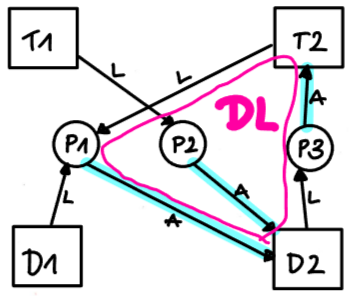
\includegraphics[width=\linewidth]{deadlock_resource_graph.png}
    \end{minipage}
    \begin{minipage}{0.58\linewidth}    
    \textbf{Analyse:}
    \begin{itemize}
        \item P1 hält D1, möchte T2 und D2
        \item P2 hält T1, möchte D2  
        \item P3 hält D2, möchte T2
    \end{itemize}
    
    Es entsteht ein Zyklus: P1 $\rightarrow$ D2 $\rightarrow$ P3 $\rightarrow$ T2 $\rightarrow$ P1\\
    
    \textbf{Bedingungen für Deadlock:}
    \begin{itemize}
        \item Mutual Exclusion: Ressourcen werden exklusiv alloziert
        \item No Preemption: Ressourcen können nicht weggenommen werden
        \item Hold \& Wait: Prozesse halten Ressourcen und warten auf weitere
        \item Circular Wait: Es gibt einen Zyklus im Ressourcengraph
    \end{itemize}
    
    Alle vier Bedingungen sind erfüllt $\rightarrow$ Deadlock!
    \end{minipage}
\end{example2}

\raggedcolumns

\begin{KR}{Deadlock Detection in Resource Allocation Graphs}
    \paragraph{Resource Graph erstellen}
    \begin{itemize}
        \item Kreise: Prozesse (P1, P2, P3, ...)
        \item Rechtecke: Ressourcen (R1, R2, R3, ...)
        \item Pfeile von Prozess zu Ressource: Reqüst (Anforderung)
        \item Pfeile von Ressource zu Prozess: Allocation (Zuteilung)
    \end{itemize}
    
    \paragraph{Deadlock-Analyse}
    \begin{itemize}
        \item Suche nach Zyklen im Graph
        \item Ein Zyklus bedeutet Deadlock bei Single-Instance Ressourcen
        \item Bei Multi-Instance Ressourcen: Prüfe ob alle Instanzen blockiert
    \end{itemize}
    
    \paragraph{Deadlock-Bedingungen prüfen}
    \begin{itemize}
        \item Mutual Exclusion: Exklusive Ressourcennutzung
        \item Hold \& Wait: Halten und gleichzeitig warten
        \item No Preemption: Keine Unterbrechung möglich
        \item Circular Wait: Zyklische Warteabhängigkeiten
    \end{itemize}
    
    \paragraph{Lösungsansätze}
    \begin{itemize}
        \item Prevention: Eine der vier Bedingungen verhindern
        \item Avoidance: Banker's Algorithm
        \item Detection \& Recovery: Deadlock erkennen und auflösen
    \end{itemize}
\end{KR}

\raggedcolumns
\columnbreak

\subsection{Synchronization with Semaphores}

\begin{KR}{Synchronization Problem Solving}
    \begin{itemize}
        \item Identify critical sections
        \item Determine synchronization requirements
        \item Choose appropriate mechanism (mutex, semaphore, monitor)
        \item Ensure deadlock avoidance
        \item Test for race conditions
    \end{itemize}
\end{KR}


\begin{concept}{Semaphores}
    \begin{itemize}
        \item Semaphores are synchronization primitives used to control access to shared resources.
        \item They can be binary (0 or 1) or counting (any non-negative integer).
        \item Operations: 
            \begin{itemize}
                \item \texttt{wait(S)}: Decrement the semaphore S. If S is less than 0, block the process.
                \item \texttt{signal(S)}: Increment the semaphore S. If S was negative, wake up a blocked process.
            \end{itemize}
    \end{itemize}
\end{concept}

\begin{KR}{Semaphore-basierte Synchronisation}
    \paragraph{Semaphore verstehen}
    \begin{itemize}
        \item Semaphore S ist ein Zähler mit atomaren Operationen
        \item down(S) oder P(S): Dekrementiert S, blockiert bei S $\leq$  0
        \item up(S) oder V(S): Inkrementiert S, weckt wartende Prozesse
        \item Initialisierung bestimmt verfügbare Ressourcen
    \end{itemize}
    
    \paragraph{Synchronisationsmuster}
    \begin{itemize}
        \item Mutual Exclusion: Binary Semaphore (0/1) um kritische Bereiche
        \item Signaling: Ein Prozess signalisiert einem anderen (Producer-Consumer)
        \item Rendezvous: Zwei Prozesse warten aufeinander
        \item Barrier: Mehrere Prozesse warten aufeinander
    \end{itemize}
    
    \paragraph{Typische Synchronisationsprobleme}
    \begin{itemize}
        \item Producer-Consumer: Buffer-Management mit vollen/leeren Plätzen
        \item Reader-Writer: Mehrere Leser oder ein Schreiber
        \item Dining Philosophers: Deadlock-Vermeidung bei zyklischen Abhängigkeiten
        \item Barrier Synchronization: Alle warten aufeinander
    \end{itemize}
    
    \paragraph{Implementierungsschritte}
    \begin{itemize}
        \item Identifiziere Synchronisationspunkte
        \item Bestimme benötigte Semaphore und deren Initialisierung
        \item Verwende down() vor kritischen Bereichen/Warten
        \item Verwende up() nach kritischen Bereichen/Signaling
        \item Teste auf Deadlock-Freiheit und korrekte Reihenfolge
    \end{itemize}
\end{KR}

\begin{example2}{Semaphore Implementation}\\
    Gegeben sind drei Prozess P0, P1, und P2 die nach folgendem Schema abgearbeitet werden soll:\\
    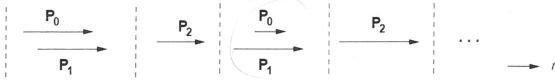
\includegraphics[width=0.8\linewidth]{semaphore_mt12.png}
    
    Die Verarbeitung startet mit den beiden Prozessen P0 und P1, die parallel verarbeitet werden sollen (es spielt kein Rolle, welcher der beiden Prozesse zürst mit seiner Verarbeitung beginnt oder aufhört). Wenn beide Prozesse eine Iteration ihrer Funktion working(x) beendet haben, folgt Prozess P2, etc.
    
    Schreiben Sie Pseudocode mit maximal 3 Semaphoren S0, S1 und S2, der garantiert, dass die oben skizzierte Reihenfolge eingehalten wird. Verwenden Sie dazu ausschliesslich Befehle der Form up(S0) und down(S0), etc. Geben Sie an, wie die Semaphore initialisiert werden müssen.
    
    \tcblower

    \begin{minipage}{0.56\linewidth}
    
    \begin{center}
    \begin{tabular}{|l|l|l|}
    \hline
    \textbf{P0} & \textbf{P1} & \textbf{P2} \\
    \hline
    Sem S0: 1 &  & \\
    Sem S1: 1 &  & \\
    Sem S2: 0 &  & \\
    \hline
    while(1) \{ & while(1) \{ & while(1) \{ \\
    \quad \quad down(S0); & \quad \quad down(S1); & \quad \quad down(S2); \\
    \quad \quad working(0); & \quad \quad working(1); & \quad \quad working(2); \\
    \quad \quad up(S2); & \quad \quad up(S2); & \quad \quad up(S0); \\
    \} & \} & \quad \quad up(S1); \\
     &  & \} \\
    \hline
    \end{tabular}
    \end{center}
    \end{minipage}
    \begin{minipage}{0.42\linewidth}
    
    \textbf{Initialisierung:}
    \begin{itemize}
        \item S0 = 1 (P0 kann starten)
        \item S1 = 1 (P1 kann starten) 
        \item S2 = 0 (P2 muss warten - Synchronisation zwischen P0/P1 und P2)
    \end{itemize}
    
    \textbf{Ablauf:}
    \begin{itemize}
        \item P0 und P1 starten parallel
        \item Beide signalisieren mit up(S2) wenn fertig
        \item P2 wartet mit down(S2) bis beide P0 und P1 fertig sind
        \item P2 gibt mit up(S0) und up(S1) die nächste Runde frei
    \end{itemize}
    \end{minipage}
\end{example2}

\subsubsection{Producer-Consumer Problem}

\begin{KR}{Producer-Consumer pattern}
    \begin{itemize}
        \item Identify shared resource (buffer)
        \item Determine capacity constraints
        \item Create semaphores for available/used slots
        \item Producer: wait(empty), produce, signal(full)
        \item Consumer: wait(full), consume, signal(empty)
    \end{itemize}
\end{KR}


\begin{example2}{Producer-Consumer Problem}
    Implement a semaphore-based solution for the producer-consumer problem:

    \begin{minipage}{0.56\linewidth}

\begin{lstlisting}[language=C, style=basesmol]
const int N = 4;      // Maximum buffer size
int sem_write = N;    // Semaphore for write slots
int sem_read = 0;     // Semaphore for read slots

// Producer process
while(1) {
    wait(sem_write);  // Wait for empty slot
    write(value);     // Write to buffer
    signal(sem_read); // Signal data available
}

// Consumer process  
while(1) {
    wait(sem_read);   // Wait for data
    read(value);      // Read from buffer
    signal(sem_write);// Signal slot available
}
\end{lstlisting}
    \end{minipage}
    \hspace{2mm}
    \begin{minipage}{0.4\linewidth}
    \textbf{Key points:}
    \begin{itemize}
        \item sem\_write tracks empty buffer slots
        \item sem\_read tracks filled buffer slots
        \item Producer waits for empty slots, signals filled slots
        \item Consumer waits for filled slots, signals empty slots
    \end{itemize}
    \end{minipage}
\end{example2}



	\raggedcolumns
	\pagebreak
	\section{Scheduling}

\mult{2}

\begin{definition}{Scheduling Problem Domain}\\
    Scheduling is a resource-time management activity:
    \begin{itemize}
        \item Focuses on managing CPU time allocation among processes
        \item Requirements vary by platform (mobile vs. supercomputer)
        \item Requirements vary by application type (batch processing vs. real-time)
    \end{itemize}
    
    Processes can be categorized by behavior:
    \begin{itemize}
        \item \textbf{CPU-bound}: Computationally intensive tasks (e.g., image processing)
        \item \textbf{I/O-bound}: Tasks that frequently wait for I/O operations (e.g., interactive applications)
    \end{itemize}
\end{definition}

\begin{concept}{When to Schedule}
    \begin{itemize}
        \item When a new process is created
        \item When a process exits
        \item When a process blocks on I/O
        \item When an I/O interrupt occurs
        \item Regularly on a timer
    \end{itemize}
    
    Based on when scheduling occurs,\\ schedulers can be:
    \begin{itemize}
        \item \textbf{Non-preemptive}: Only schedules when a process blocks or terminates
        \item \textbf{Preemptive}: Can interrupt a running process and schedule another
    \end{itemize}
\end{concept}

\begin{lemma}{Queueing Theory} base of Scheduling
    \begin{itemize}
        \item Deals with waiting for and dispatching resources
        \item Aims to provide sufficient resources to avoid under-capacity
        \item Ensures urgent tasks are not kept waiting
    \end{itemize}
\end{lemma}

\begin{theorem}{Scheduling Queues} Several Types:
    \begin{itemize}
        \item \textbf{Ready queue}: Processes waiting to be executed
        \item \textbf{Device queues}: \\ Processes waiting for specific devices
        \item \textbf{Job queue}: All processes in the system
    \end{itemize}
    
    The scheduler sorts the ready queue according to policy, and the dispatcher moves the process from the head of the queue to the CPU.
\end{theorem}

\begin{corollary}{Scheduling Metrics} used to evaluate performance:
    \begin{itemize}
        \item \textbf{CPU utilization}: \\ Keeping the CPU as busy as possible
        \item \textbf{Throughput}: \\ Number of processes completed per time unit
        \item \textbf{Turnaround time}: \\ Time from submission to completion
        \item \textbf{Waiting time}: Time spent in the ready queue
        \item \textbf{Response time}: \\ Time from request to first response
        \item \textbf{Fairness}: Equal distribution of CPU time
    \end{itemize}
\end{corollary}



\multend



\subsection{Scheduling Algorithms}

\mult{2}

\begin{definition}{Simple Schedulers}
    \begin{itemize}
        \item \textbf{Uniprocessing}: One machine, one task - no scheduler required
        \item \textbf{Multiprocessing}: Single task running at one time with job control
        \item \textbf{Multitasking}: Multiple tasks running with scheduler
    \end{itemize}
\end{definition}

\begin{concept}{Multi-level Schedulers} address priority needs:
    \begin{itemize}
        \item Multiple queues with different priorities
        \item Round Robin within each queue
        \item Challenge: High-priority tasks can cause starvation of low-priority tasks
    \end{itemize}
    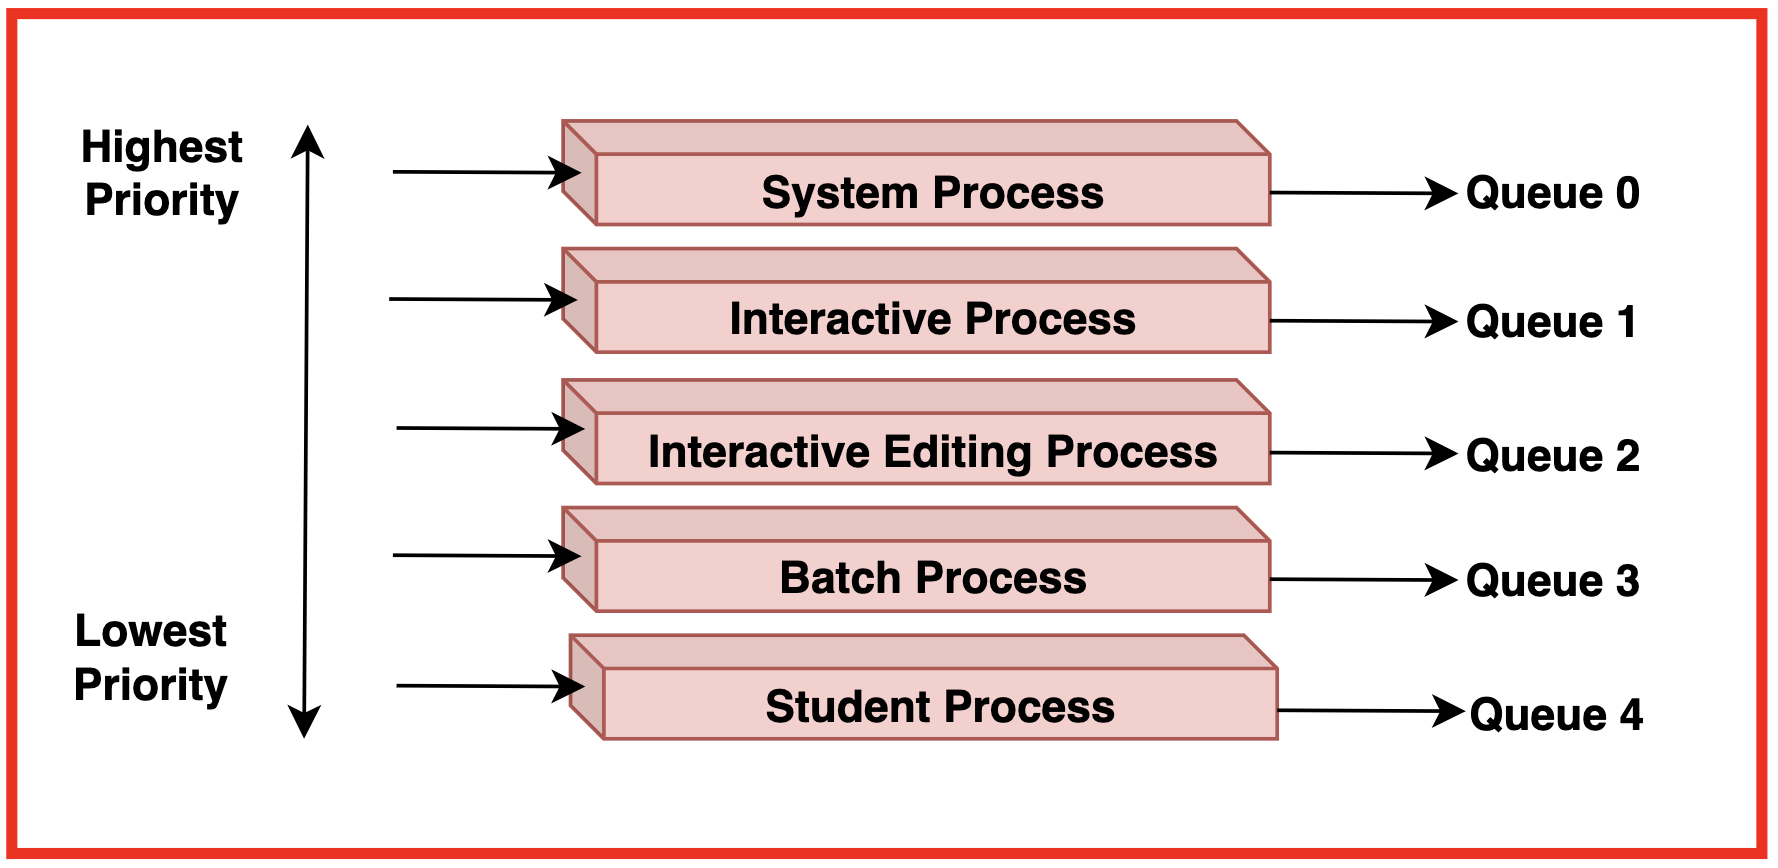
\includegraphics[width=\linewidth]{multilevel_queue.png}
\end{concept}

\begin{definition}{Fair Share Scheduling} aim for equal CPU time:
    \begin{itemize}
        \item Maintains a running clock of CPU time used per process
        \item Uses a Virtual Clock (VC) to track usage
        \item Ensures average run-time is roughly equal for all tasks
        \item Better balance between CPU-bound and I/O-bound tasks
    \end{itemize}
\end{definition}

\begin{concept}{Multi-level Feedback Queues} \\
    Addresses starvation (tasks move between queues):
    \begin{itemize}
        \item Task priority sinks after each execution interval
        \item Low-priority queues may get larger time quantum
        \item Balances responsiveness with throughput
    \end{itemize}
    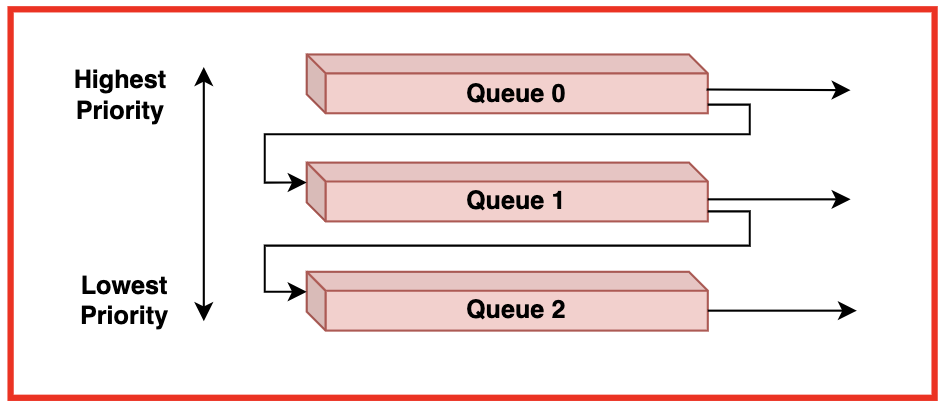
\includegraphics[width=\linewidth]{multilevel_feedback_queue.png}
\end{concept}



\multend

\mult{2}

\begin{formula}{First-In-First-Out (FIFO/FCFS)} \\ basic scheduling algorithm: 
    \begin{itemize}
        \item Processes are executed in the order they arrive
        \item Single queue, no preemption
        \item Processes run to completion
        \item Simple to implement
        \item Non-preemptive
        \item No awareness of process type (interactive vs. batch)
    \end{itemize}
    $\rightarrow$ also known as First-Come-First-Served (FCFS)

    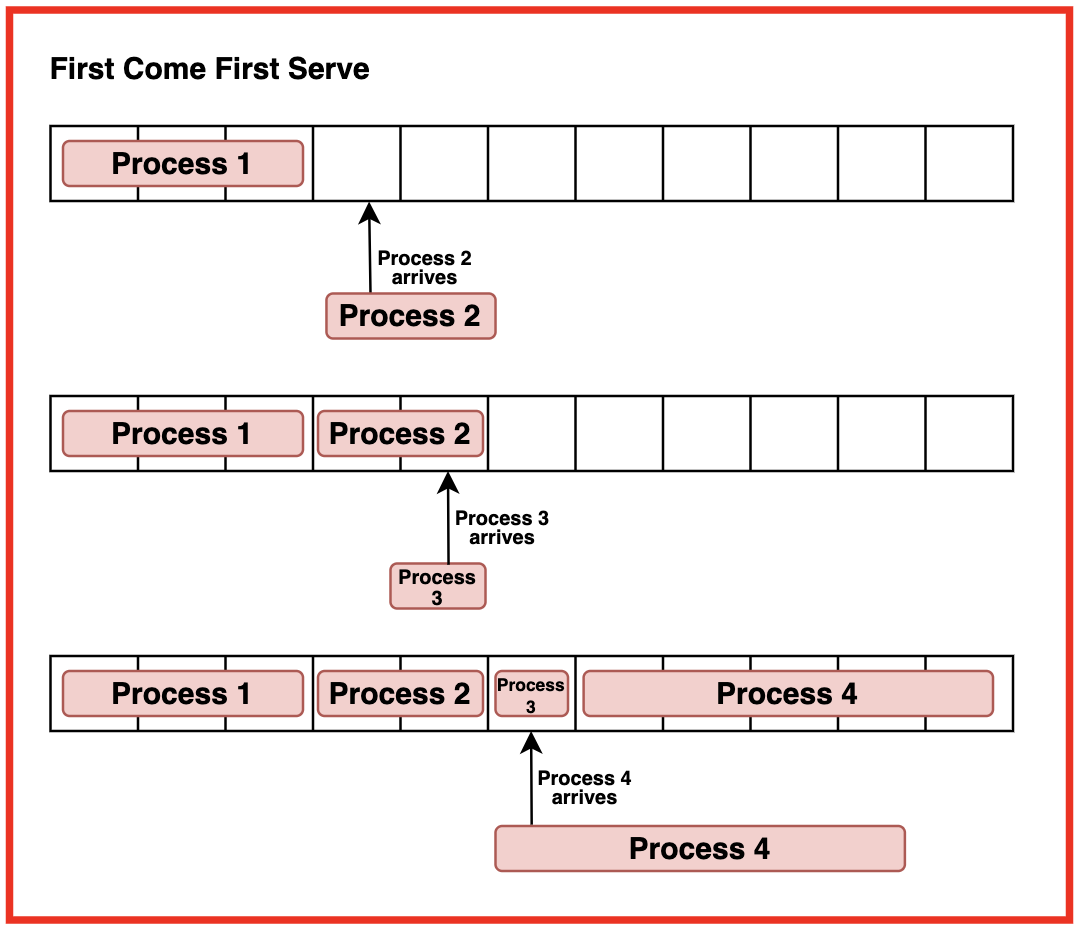
\includegraphics[width=\linewidth]{fifo_algorithm.png}
\end{formula}

\begin{formula}{Round Robin (RR)} time-sharing algorithm:
    \begin{itemize}
        \item Each process runs for a fixed time slice \\(quantum)
        \item After quantum expires, process is moved to the end of the queue
        \item Preemptive, as running tasks are interrupted after quantum
        \item Arriving tasks have priority over adjourned tasks (by convention)
        \item No starvation, as all processes eventually get CPU time
        \item Performance depends on quantum size
            \begin{itemize}
                \item Too large: approaches FIFO
                \item Too small: too much context switching overhead
            \end{itemize}
    \end{itemize}
    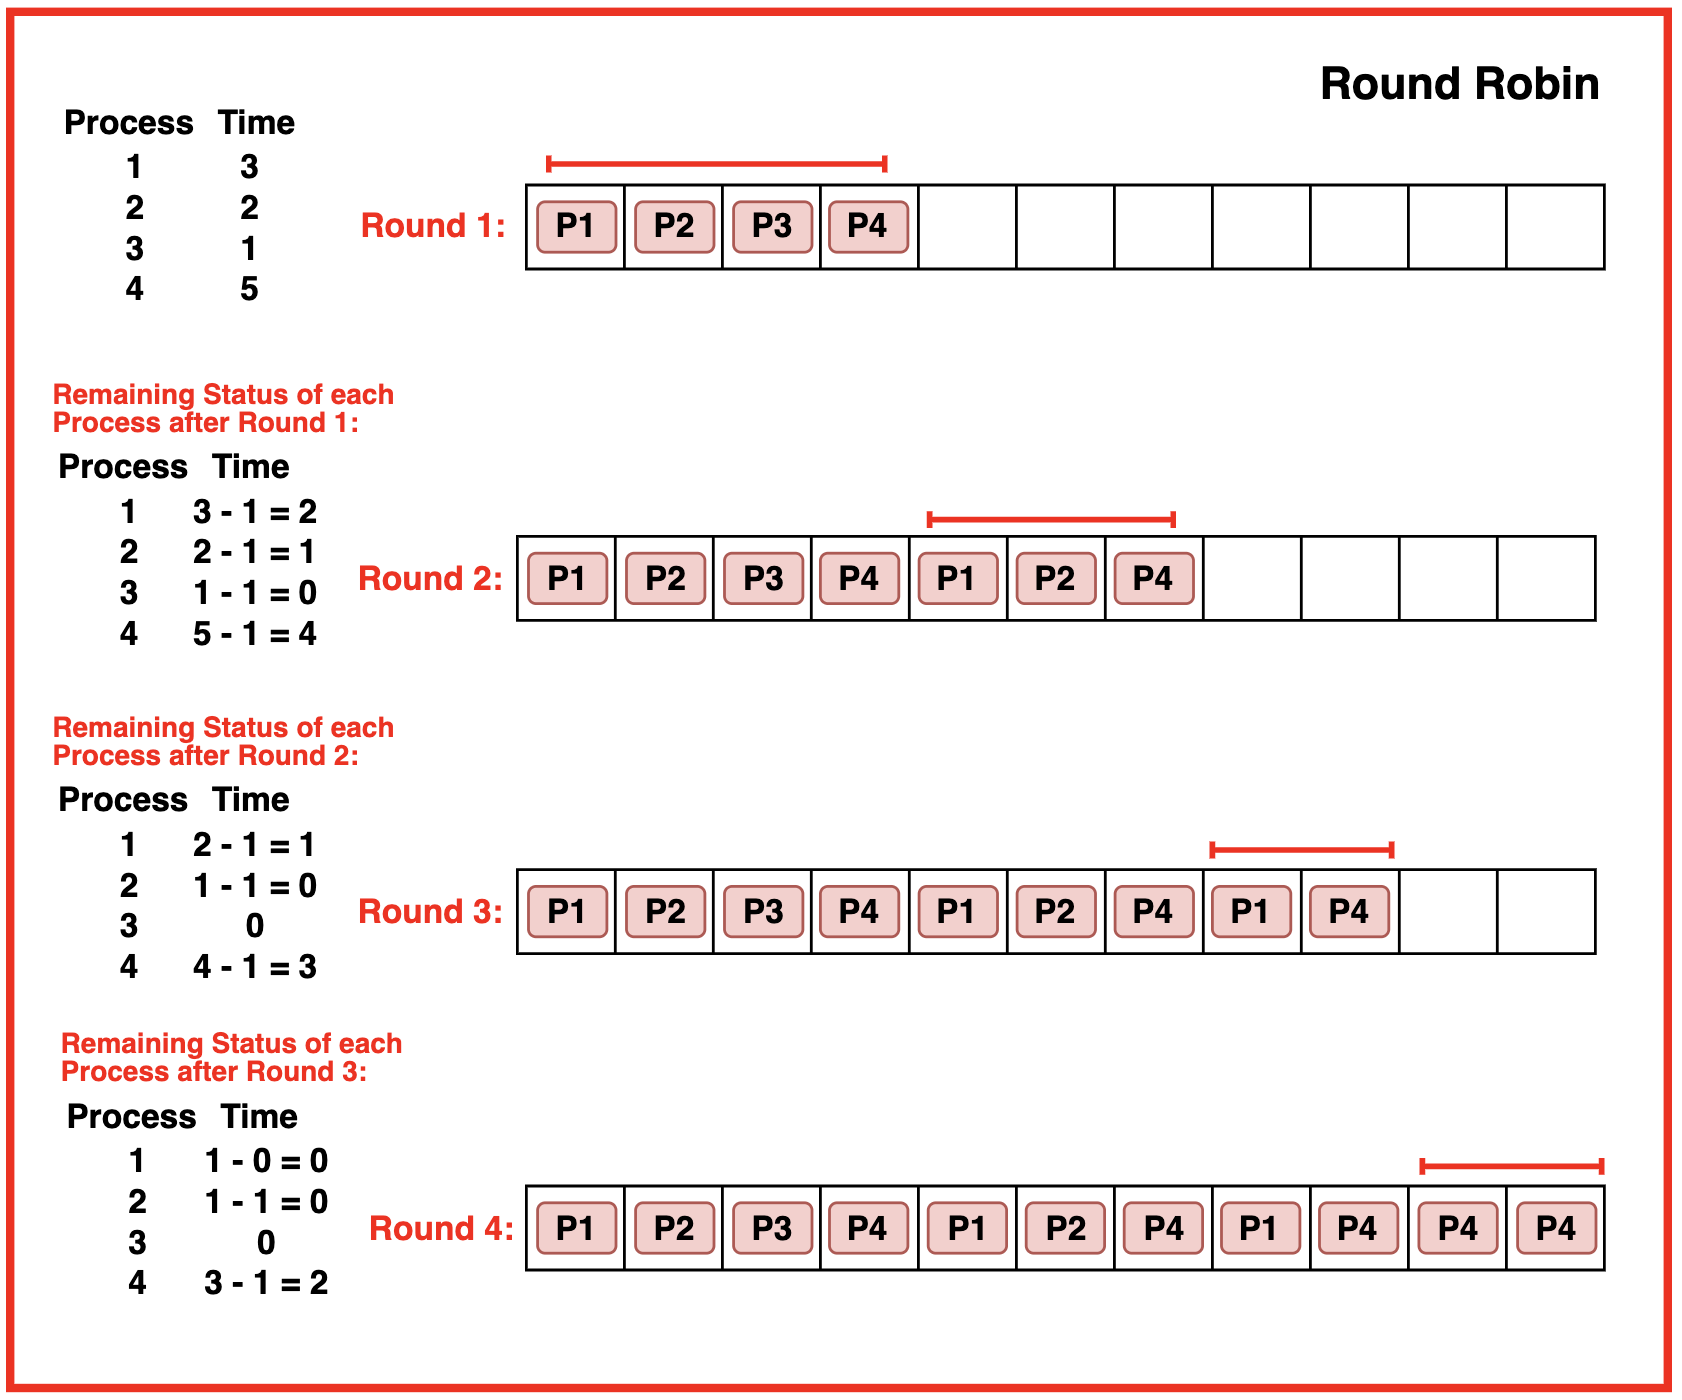
\includegraphics[width=\linewidth]{rr_algorithm.png}
\end{formula}

\begin{formula}{Shortest Job First (SJF)} \\ non-preemptive scheduling algorithm:
    \begin{itemize}
        \item Selects the process with the shortest burst time
        \item Minimizes average waiting time
        \item Non-preemptive, runs to completion
        \item Can lead to starvation for longer processes
        \item Optimal for average turnaround time
    \end{itemize}
    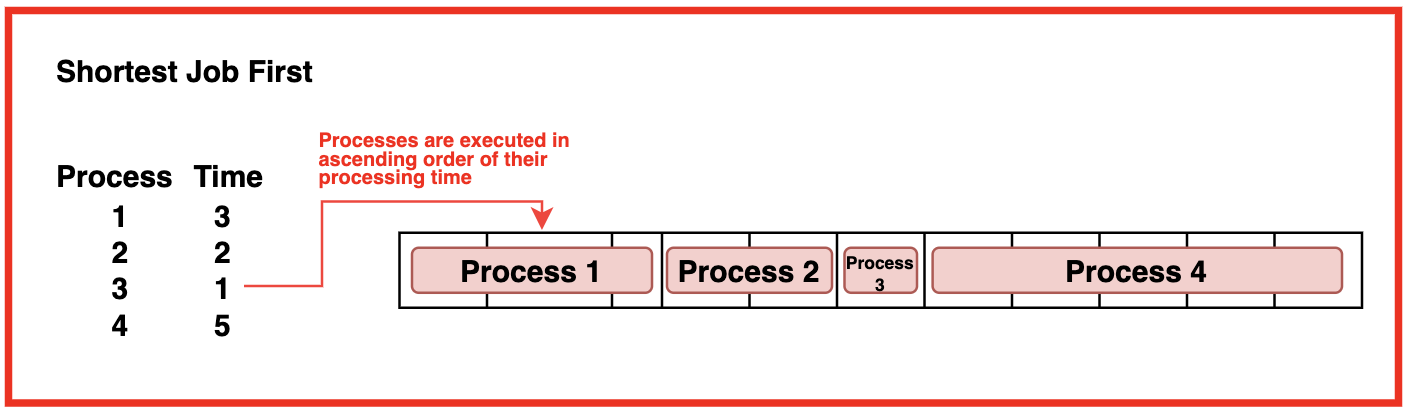
\includegraphics[width=\linewidth]{sjf_algorithm.png}
\end{formula}

\begin{formula}{Shortest Remaining Time (SRT)} \\ preemptive version of SJF:
    \begin{itemize}
        \item At each time unit, selects the process with the shortest remaining time
        \item Preempts running processes if a new process arrives with shorter remaining time
        \item Can lead to high context switching overhead
        \item Optimal for minimizing average waiting time
    \end{itemize}
   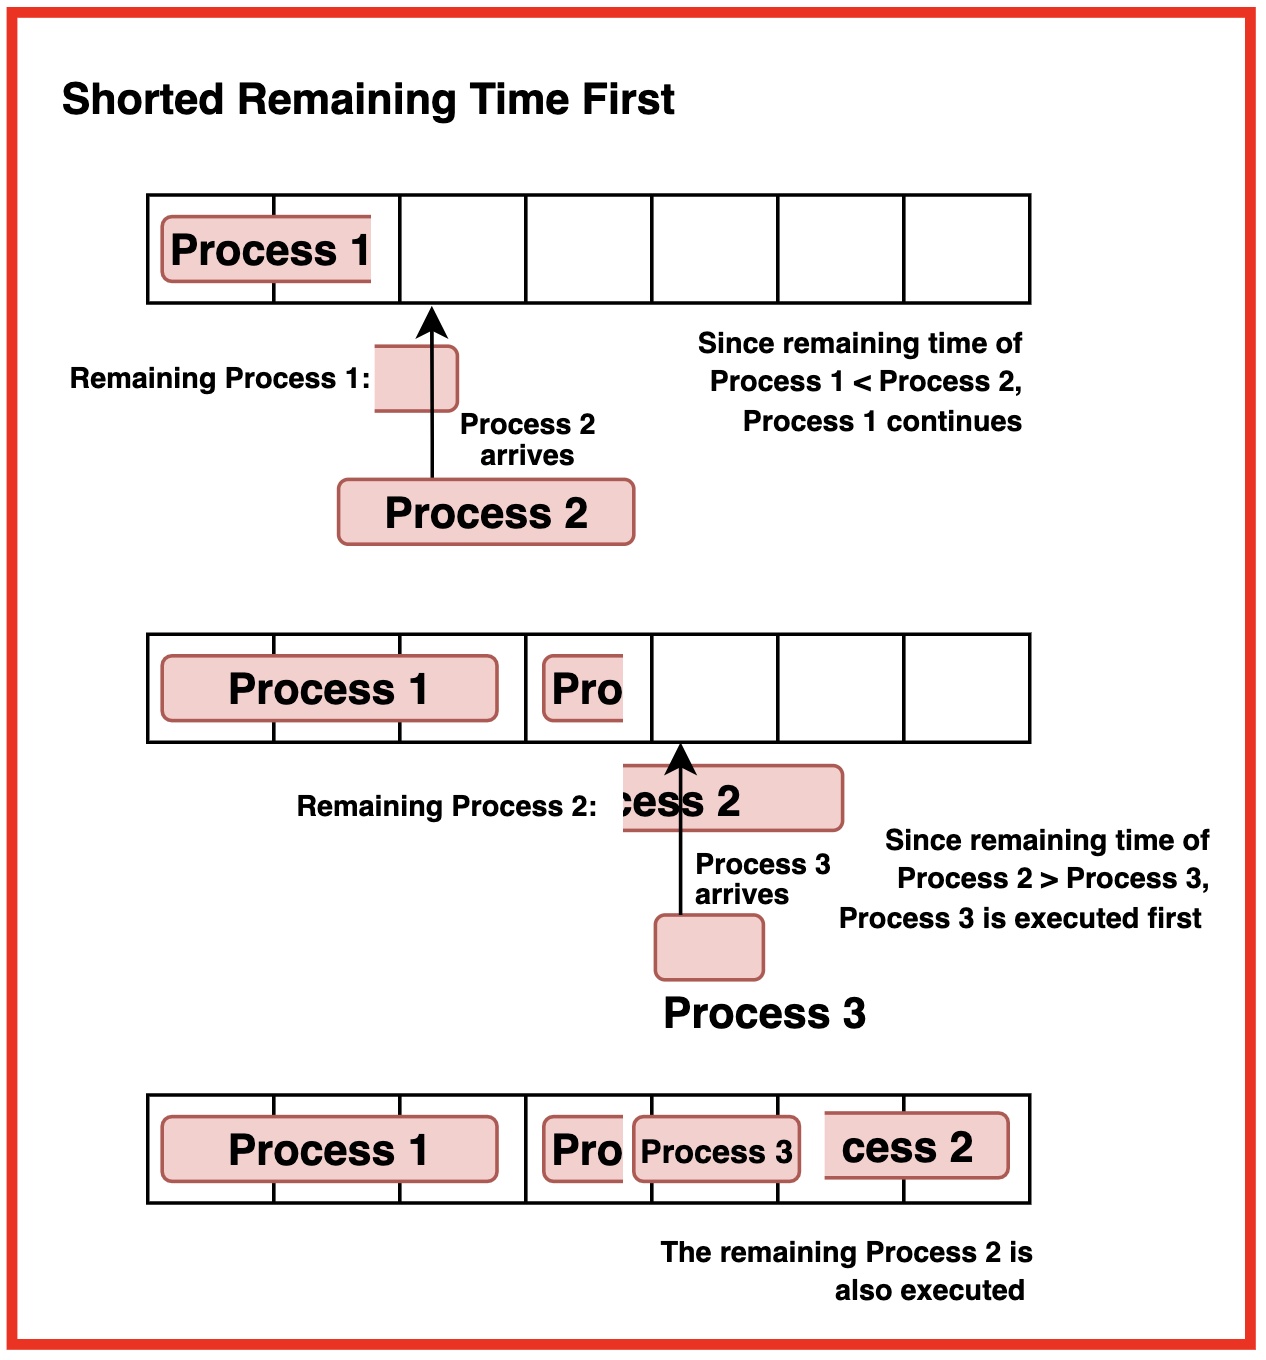
\includegraphics[width=\linewidth]{srt_algorithm.png}
\end{formula}





\begin{example2}{FIFO and RR Scheduling Comparison}\\
    Given the following task list:
    
    \begin{tabular}{|c|c|c|}
        \hline
        Task & Arrival Time & Burst Time \\
        \hline
        T1 & 0 & 10 \\
        T2 & 3 & 6 \\
        T3 & 7 & 1 \\
        T4 & 8 & 3 \\
        \hline
    \end{tabular}
    
    \textbf{FIFO Schedule}:
    
    T1 runs from 0-10, T2 runs from 10-16, T3 runs from 16-17, T4 runs from 17-20
    
    \textbf{Round Robin Schedule} (quantum = 2):
    
    T1(0-2), T1(2-4), T2(4-6), T1(6-8), T2(8-10), T3(10-11), T4(11-13), \\ T1(13-15), T2(15-17), T1(17-19), T1(19-20)
    
    RR provides better response time but potentially longer turnaround time due to context switches.
\end{example2}

\multend

\subsubsection{Scheduling Algorithm Analysis}

\mult{2}

\begin{KR}{Scheduling Algorithm Analysis}
    \paragraph{FIFO/FCFS approach}
    \begin{itemize}
        \item Execute processes in arrival order
        \item Non-preemptive
        \item Simple but may cause long wait times
    \end{itemize}
    
    \paragraph{SJF approach}
    \begin{itemize}
        \item At decision point, choose process with shortest total time
        \item Non-preemptive
        \item Optimal for average waiting time
    \end{itemize}
    
    \paragraph{SRT approach}
    \begin{itemize}
        \item At each time unit, choose process with shortest remaining time
        \item Preemptive version of SJF
        \item May cause frequent context switches
    \end{itemize}
    
    \paragraph{Problem-solving steps}
    \begin{itemize}
        \item Create timeline showing all events (arrivals, completions)
        \item For each algorithm, trace through decision points
        \item Calculate metrics: turnaround time, waiting time, response time
    \end{itemize}
\end{KR}



\begin{KR}{Round Robin Analysis}
    \paragraph{Quantum size considerations}
    \begin{itemize}
        \item Too large: Approaches FIFO, poor response time
        \item Too small: High context switching overhead
        \item Optimal: Slightly larger than typical interaction time
    \end{itemize}
    
    \paragraph{Performance factors}
    \begin{itemize}
        \item Context switch overhead
        \item Interactive response requirements
        \item CPU-bound vs. I/O-bound process mix
        \item System throughput vs. responsiveness trade-off
    \end{itemize}
\end{KR}

\begin{example2}{Round Robin Scheduling}
    Why should the time quantum be larger than typical interaction time?
    
    \textbf{Reason:}
    If the quantum is larger than interaction processing time, the entire user interaction can be completed within one quantum. This ensures the system responds quickly to user input without interrupting the interactive process.
    
    If the quantum is too small, interactive processes get interrupted before completing their response, leading to poor user experience.
\end{example2}

\multend

\begin{example2}{FIFO{,} SJF{,} and SRT Scheduling}
    Given processes with arrival and burst times, determine execution order:

    \begin{minipage}{0.35\linewidth}    
    \begin{tabular}{|c|c|c|}
        \hline
        Process & Arrival T. & Burst T. \\
        \hline
        P & 0 & 10 \\
        Q & 4 & 5 \\
        R & 5 & 10 \\
        S & 6 & 1 \\
        \hline
    \end{tabular}
    \end{minipage}
    \begin{minipage}{0.65\linewidth}    
    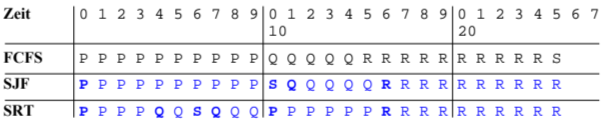
\includegraphics[width=\linewidth]{SCHEDULING_sep07.png}
    \end{minipage}
\end{example2}

\subsubsection{Multi-level Scheduling}

\begin{KR}{Priority-Based Multi-Level Scheduling}
    \paragraph{Organize by priority levels}
    \begin{itemize}
        \item Group processes by priority (higher number = higher priority)
        \item Maintain separate ready queue for each priority level
        \item Always schedule from highest priority non-empty queue
    \end{itemize}
    
    \paragraph{Apply Round Robin within priority}
    \begin{itemize}
        \item Use time quantum for processes at same priority level
        \item Move process to end of same priority queue when quantum expires
        \item New arrivals join appropriate priority queue
    \end{itemize}
    
    \paragraph{Handle preemption}
    \begin{itemize}
        \item Higher priority process always preempts lower priority
        \item Preemption occurs immediately when higher priority task arrives
        \item Preempted task returns to head of its priority queue
    \end{itemize}
\end{KR}

\begin{minipage}{0.45\linewidth}

\begin{theorem}{Priority-Based Scheduling Issues}
    \begin{itemize}
        \item Priority inversion
        \item Starvation of low-priority processes
        \item Priority assignment difficulties
        \item Real-time deadline misses
    \end{itemize}
    
    \textbf{Solution approaches:}
    \begin{itemize}
        \item Priority inheritance protocols
        \item Aging mechanisms
        \item Fair-share scheduling
        \item Deadline-based scheduling
    \end{itemize}
\end{theorem}
\end{minipage}
\begin{minipage}{0.55\linewidth}

\begin{example}
    \textbf{Priority inversion occurs when:}
    \begin{itemize}
        \item High-priority process waits for low-priority process
        \item Medium-priority processes preempt low-priority process
        \item High-priority process effectively blocked by medium-priority processes
    \end{itemize}
    
    \textbf{Prevention methods:}
    \begin{itemize}
        \item \textbf{Priority inheritance}: Low-priority process temporarily inherits high priority
        \item \textbf{Priority ceiling}: Resources assigned maximum priority of potential users
        \item \textbf{Dynamic priority adjustment}: Increase priority of waiting processes over time
    \end{itemize}
\end{example}
\end{minipage}




\begin{KR}{Multi-Level Round Robin Scheduling}

    \begin{minipage}{0.6\linewidth}
    \paragraph{Multi-level principles}
    \begin{itemize}
        \item Separate queues for different priority levels
        \item Higher priority queues are served first
        \item Round robin within each priority level
        \item Lower priority tasks only run when higher queues are empty
    \end{itemize}
    
    \paragraph{Timeline construction}
    \begin{itemize}
        \item Mark process arrivals on timeline
        \item At each time unit, determine which process should run
        \item Apply round robin within the highest non-empty priority queue
        \item Show context switches and queue changes
    \end{itemize}
    \end{minipage}
    \hspace{2mm}
    \begin{minipage}{0.35\linewidth}
    \paragraph{Scheduling algorithm}
    \begin{itemize}
        \item Group processes by priority level
        \item Always check highest priority queue first
        \item Use round robin with specified time quantum within each queue
        \item Preemption occurs when higher priority process arrives
        \item Track remaining execution time for each process
    \end{itemize}
    \end{minipage}
\end{KR}

\begin{example2}{Multi-Level Scheduling with RR}
    Five processes with time quantum = 1:
    
    \begin{minipage}{0.45\linewidth}
    \begin{tabular}{|c|c|c|c|}
        \hline
        Process & Priority & Arrival & Execution \\
        \hline
        P1 & 0 & 0 & 4 \\
        P2 & 1 & 1 & 3 \\
        P3 & 1 & 2 & 2 \\
        P4 & 0 & 5 & 3 \\
        P5 & 0 & 7 & 2 \\
        \hline
    \end{tabular}
    \end{minipage}
    \begin{minipage}{0.55\linewidth} 
    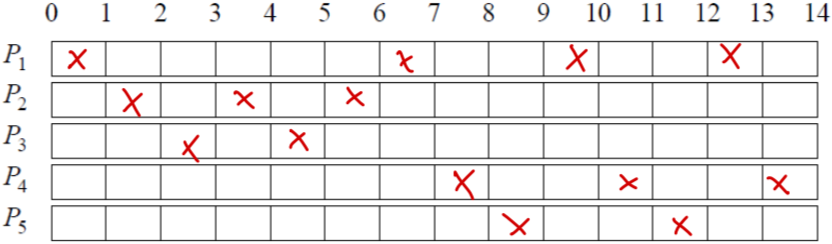
\includegraphics[width=\linewidth]{multilevelsched2.png}
    \end{minipage}
    \vspace{2mm}\\
    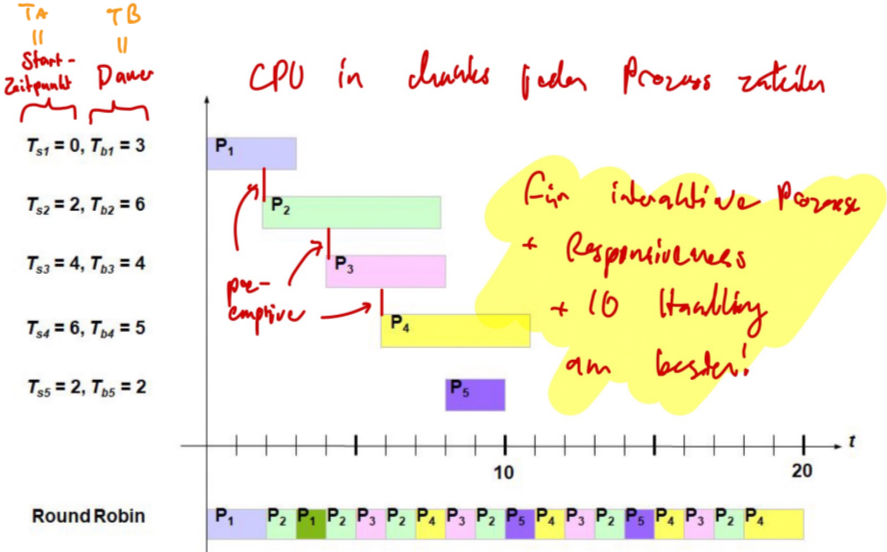
\includegraphics[width=\linewidth]{multilevel_scheduling_SEP19.png}
    \vspace{2mm}\\
    \textbf{Execution timeline:}
    \begin{itemize}
        \item t=0-1: P1 (only process available)
        \item t=1-2: P2 (higher priority, preempts P1)
        \item t=2-3: P3 (same priority as P2, P2's quantum expired)
        \item t=3-4: P2 (continues RR at priority 1)
        \item t=4-5: P3 (completes)
        \item t=5-6: P2 (completes), then P4 starts
        \item t=6-7: P1 (RR at priority 0)
        \item t=7-8: P4 (continues RR), P5 arrives
        \item And so on with RR between P1, P4, P5 at priority 0...
    \end{itemize}
\end{example2}







\subsubsection{Real-Time Schedulers}



\begin{definition}{Real-Time Systems}
    Real-time systems have specific scheduling needs:

    \begin{minipage}{0.54\linewidth}
    \begin{itemize}
        \item Need responsiveness to I/O
        \item Must fulfill deadlines (hard or soft)
        \item Hard deadlines MUST be met, soft deadlines \\can occasionally be missed
        \item Deadlines may be in milliseconds, seconds, or hours
    \end{itemize}
    \end{minipage}
    \begin{minipage}{0.45\linewidth}    
    \textbf{A Real-Time Operating System (RTOS):}
    \begin{itemize}
        \item Completes system calls in deterministic time
        \item Schedules user tasks to meet deadlines
        \item Facilitates hard real-time requirements
    \end{itemize}
    \end{minipage}
\end{definition}

\mult{2}

\begin{formula}{Rate Monotonic Scheduling}
    Static-priority \\ scheduling algorithm for real-time systems:
    \begin{itemize}
        \item Higher repetition rate tasks $\rightarrow$ higher priority 
        \item Guaranteed schedule if utilization meets criteria:
        \vspace{-2mm}\\
            $$U = \sum_{i=1}^{n} \frac{C_e}{T_r} \leq n(2^{1/n} - 1)$$
            \vspace{-2mm}\\
            \small{Where $C_e$ is execution time and $T_r$ is period}
        \item \normalsize Max. guaranteed utilization converges to \textasciitilde69\%
        \item Schedule determined at compile-time, \\ not run-time
    \end{itemize}
\end{formula}

\begin{formula}{Earliest Deadline First (EDF)}\\
    Dynamic scheduling algorithm for real-time systems:
    \begin{itemize}
        \item Scheduler determines the task with the next deadline
        \item Task with the earliest deadline gets \\ highest priority
        \item Schedule is achievable if utilization does not exceed 100\%
        \item Can achieve full CPU utilization
        \item Schedule determined at run-time, \\ not compile-time
    \end{itemize}
\end{formula}

\multend

\begin{example2}{Rate Monotonic Scheduling}
    Given tasks with the following characteristics:
    
    \begin{tabular}{|c|c|c|}
        \hline
        Task & WCET (C) & Period (T) \\
        \hline
        T1 & 10 & 20 \\
        T2 & 10 & 50 \\
        T3 & 5 & 30 \\
        \hline
    \end{tabular}
    
    \tcblower
    
    \textbf{Analysis}:\\
    1. T1 has the highest priority (shortest period)\\
    2. Utilization: $U = \frac{10}{20} + \frac{10}{50} + \frac{5}{30} = 0.5 + 0.2 + 0.167 = 0.867$\\
    3. Maximum utilization for 3 tasks: $3(2^{1/3} - 1) \approx 0.779$\\
    4. Since $0.867 > 0.779$, there is no guaranteed schedule\\    
    However, a feasible schedule might still exist. Testing would be required to confirm.
\end{example2}

\begin{example2}{Rate Monotonic Scheduling Example}\\
    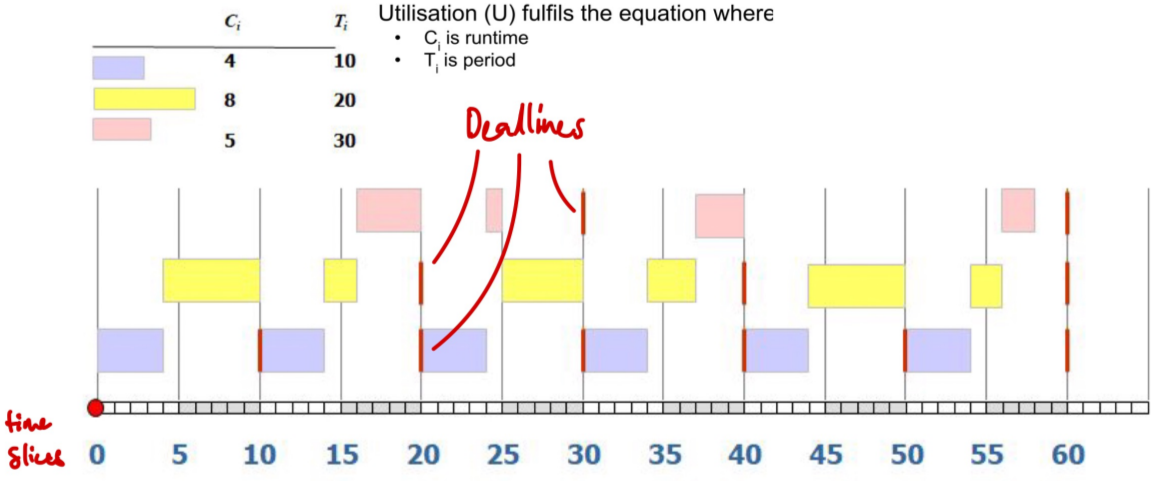
\includegraphics[width=\linewidth]{general_scheduling_example.png}
\end{example2}

\begin{minipage}{0.53\linewidth}
\begin{KR}{Earliest Deadline First Scheduling}
    \paragraph{EDF Algorithm principles}
    \begin{itemize}
        \item Always schedule the task with the earliest deadline
        \item Preemption occurs when a task with earlier deadline arrives
        \item Re-scheduling happens at specified intervals or task completion
    \end{itemize}
    
    \paragraph{Scheduling steps}
    \begin{itemize}
        \item Calculate all task deadlines for the scheduling period
        \item At each scheduling point, identify available tasks
        \item Select task with earliest deadline
        \item Handle ties with specified priority rules (e.g., shorter period)
        \item Mark execution periods in timeline diagram
    \end{itemize}
    
    \paragraph{Timeline construction}
    \begin{itemize}
        \item Create timeline with scheduling intervals marked
        \item For each interval, determine which task should run
        \item Show task execution as filled blocks
        \item Verify all deadlines are met
    \end{itemize}
\end{KR}
\end{minipage}
\begin{minipage}{0.46\linewidth}
\begin{theorem}{EDF Details}
    \paragraph{Calculating absolute deadlines}
    \begin{itemize}
        \item For each task instance:\\ Deadline = Arrival time + Period
        \item Track all active tasks \\ (arrived but not completed)
        \item Update deadlines when new instances arrive
    \end{itemize}
    
    \paragraph{Scheduling by earliest deadline}
    \begin{itemize}
        \item At each scheduling point, select task with earliest absolute deadline
        \item Preempt running task if new arrival has earlier deadline
        \item Use period as tiebreaker for equal deadlines (shorter period wins)
    \end{itemize}
    
    \paragraph{Handling rescheduling points}
    \begin{itemize}
        \item Reschedule when task completes or suspends
        \item Reschedule at fixed intervals if specified
        \item Reschedule when new task arrives \\ (if preemptive)
    \end{itemize}
\end{theorem}
\end{minipage}


\begin{example2}{EDF Scheduling}
    Three periodic tasks with rescheduling every 4ms or when a task is suspended: 
    
    \begin{tabular}{|c|c|c|}
        \hline
        Task & Period & Execution Time \\
        \hline
        \textcolor{red}{T1} & 4ms & 1ms \\
        \textcolor{red}{T2} & 8ms & 4ms \\
        \textcolor{red}{T3} & 12ms & 3ms \\
        \hline
    \end{tabular}

    Priority: in case of equal deadlines, shorter period wins.

    \tcblower
    \textbf{Preemptive Diagram:}\\
    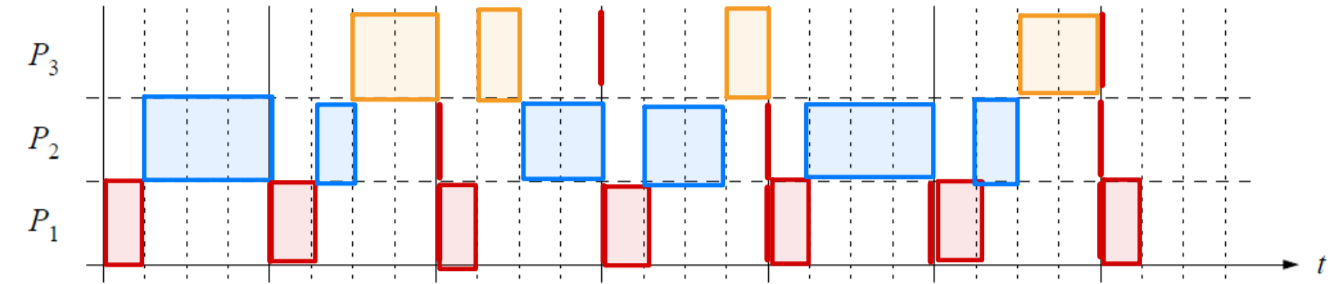
\includegraphics[width=\linewidth]{scheduling_diagram_SEP19.png}
    
    \textbf{Timeline analysis (first 24ms):}
    \begin{itemize}
        \item t=0: T1(dl=4), T2(dl=8), T3(dl=12) arrive $\rightarrow$ Schedule T1
        \item t=1: T1 completes $\rightarrow$ Schedule T2  
        \item t=4: T1(dl=8) arrives, T2 continues (dl=8, but T2 started first)
        \item t=5: T1 executes (same deadline, shorter period wins)
        \item t=6: T1 completes $\rightarrow$ Schedule T2
        \item t=8: T1(dl=12), T2(dl=16) arrive, T3 continues
        \item And so on...
    \end{itemize}
    
    The schedule ensures all deadlines are met with this task set.
\end{example2}

\raggedcolumns
\columnbreak

\subsection{Linux Scheduling}

\mult{2}

\begin{definition}{Linux Scheduling Policies}\\
    \textbf{Real-Time Policy}: For time-critical tasks
        \begin{itemize}
            \item SCHED\_DEADLINE: Earliest Deadline First + Constant Bandwidth Server
            \item SCHED\_FIFO \& SCHED\_RR (see algorithms)
        \end{itemize}
    \textbf{Normal Policy}: For regular tasks
        \begin{itemize}
            \item SCHED\_OTHER: default (CFS)
            \item SCHED\_BATCH: For batch processing tasks
            \item SCHED\_IDLE: extremely low priority bg. tasks
        \end{itemize}
\end{definition}

\begin{definition}{Linux Priority System} Kernel vs. User Space:
    \begin{itemize}
        \item \textbf{Kernel space}: Priorities from high to low
            \begin{itemize}
                \item RT: 0-99
                \item Normal: 100-139
            \end{itemize}
        \item \textbf{User space}: 'nice' values from -20 (high) to +19 (low)
            \begin{itemize}
                \item Maps to kernel priorities:\\ nice + 20 = kernel priority - 100
                \item Not used in RT policies
            \end{itemize}
    \end{itemize}
\end{definition}

\multend

\mult{2}

\begin{formula}{SCHED\_DEADLINE}
    Highest priority scheduler:
    \begin{itemize}
        \item Implements Earliest Deadline First + Constant Bandwidth Server
        \item Takes parameters: runtime, period, and deadline
        \item Tasks scheduled with this cannot fork
        \item Tasks may yield CPU time when not needed
    \end{itemize}
\end{formula}

\begin{formula}{SCHED\_FIFO}
    FIFO real-time scheduler:
    \begin{itemize}
        \item Uses one queue per priority level (1-99)
        \item Higher priority than SCHED\_RR \\ at same priority level
        \item Immediately preempts any Normal policy thread
        \item Runs to completion unless:
            \begin{itemize}
                \item Preempted by a higher priority RT thread
                \item Blocked by I/O call
                \item Voluntarily yields the CPU
            \end{itemize}
    \end{itemize}
\end{formula}

\begin{formula}{SCHED\_RR}
    Round Robin real-time scheduler:
    \begin{itemize}
        \item Similar to SCHED\_FIFO but with time quanta
        \item When quantum expires, thread moved to end of its priority queue
        \item Quantum size configurable (default 100ms)
        \item RT bandwidth limiting prevents RT tasks from monopolizing CPU
    \end{itemize}
\end{formula}

\begin{formula}{Completely Fair Scheduler (CFS)}\\
    Default scheduler in Linux (SCHED\_OTHER):
    \begin{itemize}
        \item Uses a red-black tree sorted by execution time (O(log N) operations)
        \item Tracks virtual runtime to achieve fairness
        \item Considers 'nice' values to adjust CPU share
        \item Tasks can be grouped and scheduled together
        \item Aims to model an \\ 'ideal, precise multi-tasking CPU'
        \item Time accounting managed according to configurable granularity
    \end{itemize}
\end{formula}

\begin{formula}{SCHED\_BATCH and SCHED\_IDLE}\\
    Low-priority schedulers:
    \begin{itemize}
        \item \textbf{SCHED\_BATCH}:
            \begin{itemize}
                \item Same static priority as SCHED\_OTHER
                \item Designed for batch-type, CPU-intensive tasks
                \item Applies penalty due to CPU usage
                \item SCHED\_OTHER has precedence over \\ SCHED\_BATCH at same nice value
            \end{itemize}
        \item \textbf{SCHED\_IDLE}:
            \begin{itemize}
                \item Extremely low priority
                \item Lower than static priority 0 and nice 19
                \item Used for background tasks that should only run when system is idle
            \end{itemize}
    \end{itemize}
\end{formula}

\multend

\raggedcolumns
\columnbreak

\subsection{Multi-core Scheduling}

\mult{2}

\begin{definition}{Load Balancing} on multicore systems:
    \begin{itemize}
        \item Dynamic distribution of tasks across CPU cores
        \item Applied based on scheduling policy
        \item Balances competing concerns:
            \begin{itemize}
                \item Moving tasks incurs management overhead
                \item Moving tasks incurs cache penalty \\ (lost cache advantage)
            \end{itemize}
    \end{itemize}
\end{definition}

\begin{definition}{Cache Affinity} affects scheduling decisions:
    \begin{itemize}
        \item Task data may remain in CPU cache after context switch
        \item Rerunning on the same core avoids cache misses
        \item Linux considers estimated cache live-time when migrating tasks
        \item Default cache live-time: \\ /proc/sys/kernel/sched\_migration\_cost\_ns
    \end{itemize}
\end{definition}

\multend

\begin{KR}{Analyzing Scheduling in Linux}
    \paragraph{Viewing scheduler information}
    \begin{itemize}
        \item Check process priorities: \texttt{ps -el} (PRI and NI columns)
        \item View real-time processes: \texttt{ps -eo pid,cls,pri,rtprio,nice,cmd | grep -E 'CLS|FIFO|RR'}
        \item Check scheduler statistics: \texttt{cat /proc/schedstat}
        \item See current I/O scheduler: \texttt{cat /sys/block/sda/queue/scheduler}
    \end{itemize}
    
    \paragraph{Modifying process priorities}
    \begin{itemize}
        \item Start process with nice value: \texttt{nice -n [value] command}
        \item Change nice value: \texttt{renice [value] -p [pid]}
        \item Set real-time priority: \texttt{chrt -f [priority] command} (SCHED\_FIFO)
        \item Set round-robin priority: \texttt{chrt -r [priority] command} (SCHED\_RR)
    \end{itemize}
    
    \paragraph{Analyzing schedule}
    \begin{itemize}
        \item Trace scheduling events: \texttt{trace-cmd record -e sched}
        \item View trace results: \texttt{trace-cmd report}
        \item Check CPU affinity: \texttt{taskset -p [pid]}
        \item Set CPU affinity: \texttt{taskset -c [cpu\_list] -p [pid]}
    \end{itemize}
\end{KR}




\subsubsection{Complexity Analysis}


\begin{KR}{Algorithm Complexity Analysis}
    \paragraph{Time complexity evaluation}
    \begin{itemize}
        \item O(1): Constant time, independent of input size
        \item O(log n): Logarithmic time, scales well
        \item O(n): Linear time, proportional to input size
        \item Identify bottleneck operations
    \end{itemize}
    
    \paragraph{Scheduler efficiency factors}
    \begin{itemize}
        \item Process selection time
        \item Context switch overhead
        \item Load balancing cost
        \item Priority calculation complexity
    \end{itemize}
\end{KR}

\begin{example2}{Linux O(1) Scheduler}
    Explain why the Linux O(1) scheduler is called O(1):
    
    \textbf{O(1) refers to constant time complexity:}
    \begin{itemize}
        \item Time to find next process is independent of total number of processes
        \item Uses active and expired arrays with 140 priority levels each
        \item Bitmap indicates which priority levels have waiting processes
        \item Simply finds highest priority bit set and takes first process from that queue
    \end{itemize}
    
    \textbf{Algorithm:}
    \begin{itemize}
        \item Check bitmap for highest priority with waiting processes
        \item Take first process from that priority queue
        \item Constant time regardless of system load
    \end{itemize}
\end{example2}




	\raggedcolumns
	\pagebreak
	\section{Resource Control}

\mult{2}

\begin{concept}{Resource Competition}\\
    Operating systems must manage competition\\ for resources (res.):
    \begin{itemize}
        \item \textbf{Physical resources}: \\ Devices, bus systems, memory, etc.
        \item \textbf{Virtual resources}: Timers, locks, etc.
    \end{itemize}
    
    Resource control requires:
    \begin{itemize}
        \item Visibility: Knowing what resources are available
        \item Access control: Determine who can use res.
        \item Usage monitoring: Track resource consumption
        \item Unified approach: Coordinated res. management
    \end{itemize}
\end{concept}

\begin{definition}{Nice Process Concept}\\
    Traditional Unix approach to resource control:
    \begin{itemize}
        \item Users can be 'nice' by voluntarily releasing resources
        \item Modified by the \texttt{nice} command
        \item Limitations:
            \begin{itemize}
                \item No global definition, only relative values
                \item No strict and precise enforcement
                \item Users can only modify niceness of their own processes
                \item Limited applicability to specific resources
            \end{itemize}
    \end{itemize}
\end{definition}

\multend

\subsection{Linux Control Groups (cgroups)}

\mult{2}

\begin{definition}{Control Groups (cgroups)}
    Linux kernel feature for organizing tasks into hierarchical groups:
    \begin{itemize}
        \item Allows processes to be organized and \\ controlled collectively
        \item Strict enforcement of access and usage criteria
        \item Applies to sets of processes \& all future children
        \item Controls various types of resources \\ (CPU, memory, I/O, etc.)
    \end{itemize}
\end{definition}

\begin{theorem}{cgroups Terminology}
    Key concepts in cgroups:
    \begin{itemize}
        \item \textbf{cgroup}: Collection of processes\\ bound to limits/parameters
        \item \textbf{Subsystem} (Controller): \\Kernel component related to a resource type
        \item \textbf{Hierarchy}: \\ Arrangement of cgroups in a tree structure
        \item \textbf{Resource Controller}: \\ Implements behavior for specific resource type
    \end{itemize}
    
    Various controllers have been implemented:
    \begin{itemize}
        \item CPU controller: Limits CPU time
        \item Memory controller: Limits memory usage
        \item I/O controller: Controls disk I/O
        \item Network controller: Manages network bandwidth
        \item Devices controller: Controls device access
    \end{itemize}
\end{theorem}

\begin{definition}{cgroups Hierarchy}\\
    cgroups are organized in a hierarchical structure:
    \begin{itemize}
        \item Created by making subdirectories in the cgroup filesystem
        \item Limits defined at each level of the hierarchy
        \item Limits apply throughout the sub-hierarchy
        \item Descendant cgroups cannot exceed limits of ancestor cgroups
    \end{itemize}
\end{definition}

\begin{concept}{cgroups Implementation Approach}\\
    cgroups uses a filesystem-based approach:
    \begin{itemize}
        \item Communicates with Linux kernel via filesystem
        \item Virtual filesystem, stored in RAM
        \item Provides structured, standardized operations via I/O system calls
        \item Similar approach to /proc filesystem
        \item Implementation steps:
            \begin{itemize}
                \item Create tmpfs mount
                \item Create directory
                \item Mount resource control interfaces as files in directory
                \item Configure controls by editing files
                \item Associate processes (PIDs) with control configuration
            \end{itemize}
    \end{itemize}
\end{concept}



\multend

\subsubsection{cgroups Controllers}

\mult{2}

\begin{formula}{CPU Controller} manages CPU usage:
    \begin{itemize}
        \item Controls upper and lower limits of CPU shares
        \item Lower limit guarantees minimum CPU time when system is busy
        \item Upper limit restricts CPU time in each scheduling period
        \item Does not limit CPU usage if CPUs are not busy
    \end{itemize}
\end{formula}

\begin{formula}{Cpuset Controller} manages CPU assignment:
    \begin{itemize}
        \item Binds processes to specific CPUs
        \item Allows process isolation on multi-core systems
        \item Can be used to improve cache utilization
    \end{itemize}
\end{formula}

\begin{formula}{Memory Controller} manages memory usage:
    \begin{itemize}
        \item Reports and limits process memory, kernel memory, and swap usage
        \item Sets hard and soft limits on memory consumption
        \item Can enforce OOM (Out Of Memory) killing within cgroups
    \end{itemize}
\end{formula}

\begin{formula}{Blkio Controller} manages block device I/O:
    \begin{itemize}
        \item Limits access to block devices through throttling
        \item Sets upper I/O rate limits on devices
        \item Implements proportional-weight time-based division of disk I/O
        \item Can limit both read and write operations
    \end{itemize}
\end{formula}



\multend

\begin{example2}{CPU Controller Example}
    Limiting CPU usage for a group of processes:
    
\begin{lstlisting}[language=bash, style=basesmol]
# Create a cgroup for CPU control
mkdir /sys/fs/cgroup/cpu/limited_group
# Set maximum CPU usage to 10% (100ms in a 1000ms period)
echo 100000 > /sys/fs/cgroup/cpu/limited_group/cpu.cfs_period_us
echo 10000 > /sys/fs/cgroup/cpu/limited_group/cpu.cfs_quota_us
# Add a process to the cgroup
echo $PID > /sys/fs/cgroup/cpu/limited_group/cgroup.procs
# Run a CPU-intensive task and observe it being limited
# Even on an idle system, it won't exceed 10% of one CPU
\end{lstlisting}
\end{example2}

\begin{example2}{Device Controller Example}
    Restricting access to a device:
    
\begin{lstlisting}[language=bash, style=basesmol]
# Create a cgroup for device control
mkdir /sys/fs/cgroup/devices/group0
# By default, full permissions exist
cat /sys/fs/cgroup/devices/group0/devices.list
# Output: a *:* rwm (all devices, all permissions)

# Deny access to /dev/null (major 1, minor 3)
echo 'c 1:3 rwm' > /sys/fs/cgroup/devices/group0/devices.deny
# Add the current shell to the group
echo $$ > /sys/fs/cgroup/devices/group0/tasks
# Try to use /dev/null - it will fail
echo "test" > /dev/null
# Output: bash: /dev/null: Operation not permitted
\end{lstlisting}
\end{example2}

\subsection{cgroups Versions}

\begin{concept}{cgroups v1 vs v2}
    Linux has two implementations of cgroups:

    \begin{minipage}{0.3\linewidth}
        \textbf{cgroups v1}:
            \begin{itemize}
                \item Initial release in Linux 2.6.24
                \item Rapid adoption but \\ uncoordinated development
                \item Some inconsistencies between controllers
            \end{itemize}
        \end{minipage}
        \hspace{2mm}
        \begin{minipage}{0.65\linewidth}
        \textbf{cgroups v2}:
            \begin{itemize}
                \item Added in Linux 4.5
                \item Intended to replace v1 (but v1 continues to exist for compatibility)
                \item Currently implements a subset of v1 controllers
                \item Both versions can coexist, but a controller can't be used in both simultaneously
            \end{itemize}
    \end{minipage}
\end{concept}

\mult{2}

\begin{definition}{cgroups v1} two approaches to resource control:
    \begin{itemize}
        \item \textbf{Individual Resource Control}:
            \begin{itemize}
                \item Each controller mounted against a separate filesystem
                \item One controller associated with one hierarchy
            \end{itemize}
        \item \textbf{Collective Resource Control}:
            \begin{itemize}
                \item Multiple controllers co-mounted against a single filesystem
                \item Co-mounted controllers manage the same hierarchy
            \end{itemize}
    \end{itemize}
    
    Each cgroup is represented by a directory:
    \begin{itemize}
        \item Child cgroups represented as subdirectories
        \item Configuration files under each directory
        \item Files reflect resource limits and properties
    \end{itemize}
\end{definition}

\begin{definition}{cgroups v2}
    key differences from v1:
    \begin{itemize}
        \item All mounted controllers reside in a single unified hierarchy
        \item Simplified controller set
            \begin{itemize}
                \item io (replaces blkio)
                \item memory
                \item pids
                \item perf\_event
                \item rdma
                \item cpu
                \item freezer
            \end{itemize}
        \item Supports delegation (non-privileged users can manage subtrees)
        \item Supports thread mode (thread-level control)
    \end{itemize}
\end{definition}

\multend

\begin{concept}{Tasks vs Processes in cgroups v1}\\
    cgroups v1 distinguishes between tasks and processes:
    \begin{itemize}
        \item Process can consist of multiple threads (tasks)
        \item cgroups v1 allows independent manipulation of thread cgroup membership
        \item This can cause problems for controllers like memory (all threads share an address space)
        \item This ability has been limited in cgroups v2
    \end{itemize}
\end{concept}

\subsection{Working with cgroups}

\begin{KR}{Working with cgroups}
    \paragraph{Exploring cgroups}
    \begin{itemize}
        \item List available subsystems: \texttt{cat /proc/cgroups}
        \item View cgroup hierarchy: \texttt{tree /sys/fs/cgroup}
        \item Check cgroups created by systemd: \texttt{systemd-cgls}
        \item Monitor cgroup usage: \texttt{systemd-cgtop}
    \end{itemize}
    
    \paragraph{Creating and managing cgroups}
    \begin{itemize}
        \item Create a cgroup: \texttt{mkdir /sys/fs/cgroup/[controller]/[name]}
        \item Add process to cgroup: \texttt{echo [PID] > /sys/fs/cgroup/[controller]/[name]/cgroup.procs}
        \item Set CPU limit: \texttt{echo [value] > /sys/fs/cgroup/cpu/[name]/cpu.cfs\_quota\_us}
        \item Set memory limit: \texttt{echo [value] > /sys/fs/cgroup/memory/[name]/memory.limit\_in\_bytes}
        \item Remove cgroup: \texttt{rmdir /sys/fs/cgroup/[controller]/[name]}
    \end{itemize}
    
    \paragraph{Working with systemd cgroups}
    \begin{itemize}
        \item Create transient cgroup: \texttt{systemd-run --unit=[name] --slice=[slice] [command]}
        \item Set resource limits: \texttt{systemctl set-property [unit] [property]=[value]}
        \item Example: \texttt{systemctl set-property user.slice CPUQuota=20\%}
    \end{itemize}
\end{KR}

\begin{code}{Mounting cgroups v1}
    Mounting cgroups controllers:
    
\begin{lstlisting}[language=bash, style=basesmol]
# Create a tmpfs mount for cgroups
sudo mount -t tmpfs -o size=10M tmpfs /sys/fs/cgroup

# Mount a single controller (individual resource control)
sudo mount -t cgroup -o cpu none /sys/fs/cgroup/cpu

# Co-mount multiple controllers (collective resource control)
sudo mount -t cgroup -o cpu,cpuacct none /sys/fs/cgroup/cpu,cpuacct
\end{lstlisting}

    It's not possible to mount the same controller against multiple hierarchies.
\end{code}

\begin{code}{Creating and Managing cgroups v1}
    Basic cgroup management:
    
\begin{lstlisting}[language=bash, style=basesmol]
# Create a new cgroup
mkdir /sys/fs/cgroup/cpu/cg1

# Add the current process to the cgroup
echo $$ > /sys/fs/cgroup/cpu/cg1/cgroup.procs

# Add a specific process to the cgroup
echo <PID> > /sys/fs/cgroup/cpu/cg1/cgroup.procs

# Remove a cgroup (must be empty of processes and child cgroups)
rmdir /sys/fs/cgroup/cpu/cg1
\end{lstlisting}

    When adding a process to a cgroup, all threads in the process are moved together.
\end{code}

\begin{example2}{Using systemd Resource Control}
    Controlling resource limits with systemd:
    
\begin{lstlisting}[language=bash, style=basesmol]
# View current system slices
systemctl list-units --type=slice

# Check user slice settings
systemctl show user.slice

# Limit CPU usage for all user processes to 20%
sudo systemctl set-property user.slice CPUQuota=20%

# Create a resource-limited service
cat << EOF > /etc/systemd/system/limited-service.service
[Unit]
Description=Resource Limited Service

[Service]
ExecStart=/usr/bin/sha1sum /dev/zero
CPUQuota=10%
MemoryLimit=100M

[Install]
WantedBy=multi-user.target
EOF

# Reload systemd and start the service
sudo systemctl daemon-reload
sudo systemctl start limited-service

# Monitor resource usage
systemd-cgtop
\end{lstlisting}
\end{example2}

\begin{example2}{Creating a Custom CPU Control}
    Creating a CPU affinity control from scratch:
    
\begin{lstlisting}[language=bash, style=basesmol]
# Create a tmpfs mount
sudo mkdir -p /mnt/cgroups
sudo mount -t tmpfs none /mnt/cgroups

# Mount cpuset controller
sudo mkdir -p /mnt/cgroups/cpuset
sudo mount -t cgroup -o cpuset none /mnt/cgroups/cpuset

# Create a cgroup
sudo mkdir /mnt/cgroups/cpuset/group1

# Configure required memory settings first
echo 0 > /mnt/cgroups/cpuset/group1/cpuset.mems

# Restrict to CPUs 0 and 1 only (assuming 4 CPUs)
echo "0-1" > /mnt/cgroups/cpuset/group1/cpuset.cpus

# Run CPU-intensive processes
for i in {1..4}; do
  # Create processes
  sha1sum /dev/zero &
  # Get PID and add to cgroup
  PID=$!
  echo $PID > /mnt/cgroups/cpuset/group1/cgroup.procs
  echo "Added process $PID to CPU-restricted group"
done

# Check CPU assignment with taskset
for pid in $(cat /mnt/cgroups/cpuset/group1/cgroup.procs); do
  taskset -p $pid
done
\end{lstlisting}
\end{example2}
	\raggedcolumns
	\pagebreak
	\section{Memory Management}

\mult{2}

\begin{definition}{Memory Management Introduction}\\
    Critical system resource managed by the OS:
    \begin{itemize}
        \item The Memory Manager controls \\ main memory allocation and usage
        \item Secondary memory: buffer zone (swap)
    \end{itemize}
    
    Memory is organized in a hierarchy:
    \begin{itemize}
        \item Fast cache in 1-3 layers (L1, L2, L3)
        \item Main memory (RAM) - slower but larger
        \item Secondary memory (hard disks, SSDs) \\ - for programs and files
        \item Tertiary memory (backup storage, tapes)
    \end{itemize}
\end{definition}

\begin{concept}{Memory Management Tasks}\\
    OSs handle several memory management tasks:
    \begin{itemize}
        \item Determine how much memory processes require
        \item Deciding where in memory processes are located (position of residency)
        \item Managing how long processes remain in memory (length of residency)
        \item Subdividing memory for co-existence of \\ multiple processes
        \item Handling memory fragmentation
    \end{itemize}
\end{concept}

\multend

\subsubsection{Memory Allocation Approaches}

\mult{2}

\begin{definition}{Free Space Management}\\
    Finding free space during allocation requires efficient algorithms:
    \begin{itemize}
        \item \textbf{Bitmap approach}:
            \begin{itemize}
                \item Space-efficient representation
                \item One bit per allocation unit
                \item Fast free-space finding
            \end{itemize}
        \item \textbf{Linked list approach}:
            \begin{itemize}
                \item List of free blocks
                \item Supports various placement algorithms (first/next/best fit)
            \end{itemize}
    \end{itemize}
\end{definition}

\begin{formula}{Swapping} Free Space Management:
    \begin{itemize}
        \item Secondary memory: temp. storage for processes
        \item When processes are suspended or exit, their memory is freed
        \item When processes restart, they are reloaded into memory
        \item Allows more processes to run concurrently than physical memory would permit
    \end{itemize}
\end{formula}

\multend

\mult{2}

\begin{KR}{Free Space Management}
    \paragraph{Free space management methods}
    \begin{itemize}
        \item Bitmap: Good for uniform access, fixed size
        \item Linked list: Simple but slow random access
        \item Grouping: Combines free blocks into groups
        \item Counting: Stores (address, count) pairs
    \end{itemize}
    
    \paragraph{Evaluation criteria}
    \begin{itemize}
        \item Space efficiency
        \item Access speed
        \item Implementation complexity
        \item Fragmentation handling
        \item Main memory requirements
    \end{itemize}
\end{KR}

\begin{example2}{File System Free Space Management}
    Describe two efficient methods for tracking free blocks:
    
    \textbf{Method 1: Bitmap}
    \begin{itemize}
        \item Each bit represents one block
        \item 0 = free, 1 = allocated (or vice versa)
        \item Fast scanning for free blocks
        \item Compact representation
        \item Requires main memory for efficiency
    \end{itemize}
    
    \textbf{Method 2: Free block list with (start, length) tuples}
    \begin{itemize}
        \item List of contiguous free block ranges
        \item Each entry: (starting block, number of blocks)
        \item Efficient for large contiguous areas
        \item Dynamic size based on fragmentation
    \end{itemize}
\end{example2}

\multend

\raggedcolumns
\columnbreak

\mult{2}

\begin{definition}{Memory Division and Fragmentation}
    \begin{itemize}
        \item \textbf{Static memory division}:
            \begin{itemize}
                \item Memory divided into fixed-size segments
                \item Problem: Internal fragmentation \\ (wasted space within allocated segments)
            \end{itemize}
        \item \textbf{Dynamic memory division}:
            \begin{itemize}
                \item Memory divided according to process needs
                \item Problem: External fragmentation \\ (free space becomes fragmented)
                \item Solution: Compaction (expensive operation)
            \end{itemize}
    \end{itemize}
\end{definition}


\begin{formula}{Buddy Algorithm} Division/Fragmentation:
    \begin{itemize}
        \item Memory divided into blocks of power-of-2 sizes
        \item When a request arrives, the system:
            \begin{itemize}
                \item Finds the smallest block that fits the request
                \item If no suitable block exists, splits a larger block into two 'buddies'
                \item Allocates one buddy and keeps the other free
            \end{itemize}
        \item When a block is freed, the system:
            \begin{itemize}
                \item Checks if its buddy is also free
                \item If both are free, merge into a larger block
                \item Continues merging recursively if possible
            \end{itemize}
        \item Simpler to implement than other DAC
        \item Still experiences some internal fragmentation
    \end{itemize}
\end{formula}



\multend

\begin{KR}{Buddy System Fragmentation}
    \paragraph{Determine buddy block sizes}
    \begin{itemize}
        \item For each allocation request, find smallest power-of-2 block that fits
        \item Block size = $2^{\lceil \log_2(\text{request size}) \rceil}$
    \end{itemize}
   
    \paragraph{Calculate internal fragmentation}
    \begin{itemize}
        \item Fragmentation per block = Block size - Requested size
        \item Total fragmentation \\ = Sum of all individual fragmentations
    \end{itemize}   

    \paragraph{Account for merging}
    \begin{itemize}
        \item When blocks are freed, buddies may merge
        \item Track which blocks remain allocated vs. freed
    \end{itemize}
\end{KR}



\begin{example2}{Buddy System}\\
    Ein Betriebssystem-Kernel verwaltet seine Datenbuffer mit einem Buddy System, wobei insgesamt 8MByte Speicher zur Verfügung stehen. Zur Zeit sind folgende Buffer mit 62KByte, 34KByte und 9KByte alloziert worden. Wie viel Speicher geht dabei durch interne Fragmentierung insgesamt verloren, Angabe in KByte:
    \vspace{2mm}\\
    \begin{minipage}{0.5\linewidth}
    \textbf{Buddy System alloziert in Potenzen von 2:}    
    \begin{itemize}
        \item 62 KByte $\rightarrow$ nächste 2er-Potenz: 64 KByte
        \item 34 KByte $\rightarrow$ nächste 2er-Potenz: 64 KByte  
        \item 9 KByte $\rightarrow$ nächste 2er-Potenz: 16 KByte
    \end{itemize}
    \end{minipage}
    \begin{minipage}{0.5\linewidth}
    \textbf{Interne Fragmentierung = Alloziert - Angefordert:}
    \begin{itemize}
        \item (64 - 62) = 2 KByte
        \item (64 - 34) = 30 KByte
        \item (16 - 9) = 7 KByte
    \end{itemize}
    \end{minipage}
    \vspace{2mm}\\
    Gesamt: 2 + 30 + 7 = \textbf{39 KByte} interne Fragmentierung
\end{example2}

\begin{example2}{Buddy System Analysis}
    8MB system allocates buffers: 62KB, 34KB, 9KB
    
    \textbf{Allocation analysis:}
    \begin{itemize}
        \item \textcolor{orange}{62KB} $\rightarrow$ 64KB block (internal fragmentation: 2KB)
        \item \textcolor{blue}{34KB} $\rightarrow$ 64KB block (internal fragmentation: 30KB)
        \item \textcolor{frog}{9KB} $\rightarrow$ 16KB block (internal fragmentation: 7KB)
        \item Total internal fragmentation: 2 + 30 + 7 = 39KB
    \end{itemize}

    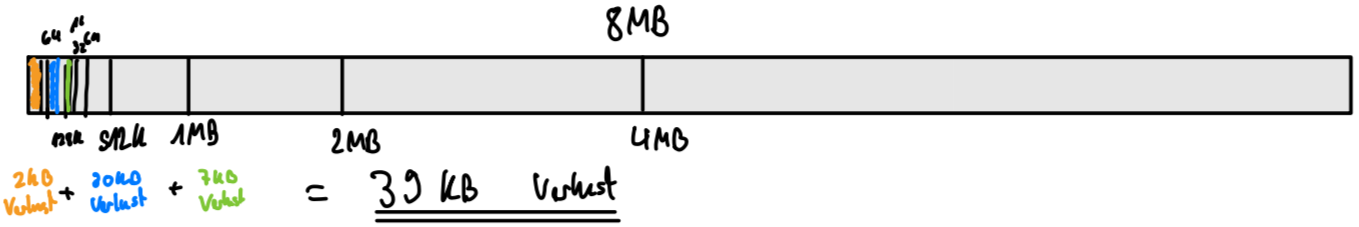
\includegraphics[width=\linewidth]{BUDDYSYSTEM_SEP19.png}
    
    The remaining memory is still available for allocation but in specific block sizes according to the buddy system structure.
\end{example2}





\columnbreak

\subsection{Virtual Memory}



\begin{definition}{Virtual Memory}\\
    Leverages program behavior characteristics:
    \begin{itemize}
        \item Programs exhibit spatial locality (tend to use a limited area of code at any time)
        \item Entire processes don't need to be fully resident in memory
        \item Non-required code/data can be swapped out when not immediately needed
        \item Enables more processes to run concurrently
        \item Must be transparent to programmer/process
    \end{itemize}
\end{definition}

\mult{2}

\begin{theorem}{Translation Lookaside Buffer (TLB)}\\
    The TLB addresses the performance overhead of \\ page table lookups:
    \begin{itemize}
        \item Cache for recently accessed page table entries
        \item Small (typically ~64 entries)
        \item Uses content-addressable memory (CAM) for fast lookups
        \item Memory access process with TLB:
            \begin{itemize}
                \item Check TLB for page number
                \item If found (TLB hit), use frame number directly
                \item If not found (TLB miss), search page table
                \item If not in page table, trigger page fault
                \item Add entry to TLB for future accesses
            \end{itemize}
    \end{itemize}
\end{theorem}

\begin{concept}{Address Translation} logical $\leftrightarrows$ physical\\
    Virtual memory requires translation between logical and pysical addresses:
    \begin{itemize}
        \item Logical address consists of page-nr. and -offset
        \item Page nr. used to look up frame nr. in page table
        \item Physical address formed by combining frame number with page offset
        \item Translation process:
            \begin{itemize}
                \item Extract page nr. and offset from logical addr.
                \item Use page nr. to index page table
                \item Retrieve frame nr. from page table
                \item Combine frame nr. with offset to form \\ physical address
            \end{itemize}
    \end{itemize}
\end{concept}



\multend

\begin{definition}{Paging} mechanism that enables virtual memory:
    \begin{itemize}
        \item Process memory is divided into fixed-size pages
        \item Physical memory is divided into frames of the same size
        \item Pages are loaded into frames as needed
        \item Memory Management Unit (MMU) manages mapping between pages and frames
        \item Typically uses 'on-demand paging' (lazy loading)
            \begin{itemize}
                \item Only loads pages when they are accessed
                \item Sometimes prefetches additional pages based on locality
            \end{itemize}
        \item Process has set of resident pages in memory
            \begin{itemize}
                \item Resident set: All process pages in memory
                \item Working set: Pages currently being used
            \end{itemize}
    \end{itemize}
\end{definition}

\mult{2}

\begin{theorem}{Page Tables} \\ Maintain mapping between pages and frames:
    \begin{itemize}
        \item Each entry contains a frame number
        \item Entries also include status bits:
            \begin{itemize}
                \item Valid bit: Indicates if page holds valid data
                \item Present bit: Indicates if page is in memory
                \item Modified bit (dirty): Indicates if page has been written to
                \item Referenced bit: Indicates recent usage
                \item Protection bits: Control read/write/execute permissions
            \end{itemize}
        \item Page tables are stored in main memory
        \item Can be very large for large address spaces
    \end{itemize}
\end{theorem}

\begin{concept}{Page Replacement}\\
    $\rightarrow$ when memory is full and a new page is needed
    \begin{itemize}
        \item System must decide which resident page to evict
        \item Can use global strategy (any process's pages) or local strategy (only faulting process's pages)
    \end{itemize}
        Common page replacement algorithms:
            \begin{itemize}
                \item Optimal: Replace page used furthest in future (theoretical only)
                \item Least Recently Used (LRU): \\ Replace page unused for longest time
                \item First-In-First-Out (FIFO): Replace oldest page
            \end{itemize}
\end{concept}


\multend

\begin{KR}{Page Table Calculations}
    \paragraph{Extract address components}
    \begin{itemize}
        \item Page Directory bits determine max number of page tables
        \item Page Number bits determine entries per page table
        \item Offset bits determine page size: $2^{\text{offset bits}}$
    \end{itemize}
    
    \paragraph{Calculate system limits}
    \begin{itemize}
        \item Page size = $2^{\text{offset bits}}$ bytes
        \item Max page tables = $2^{\text{directory bits}}$
        \item Entries per page table = $2^{\text{page number bits}}$
        \item Max frames = Max page tables $\times$ Entries per table
    \end{itemize}
\end{KR}

\begin{example2}{Page Tables}\\
    Ein Prozessor besitzt eine Wortbreite von 32Bit. Pointer (Adressen) werden in 32Bit Worten gespeichert, aber nur die 24 tieferwertigen Bits werden für die Adressbildung verwendet (Bits 25-31sind auf 0 gesetzt).
    
    Die logische Adresse ist wie folgt strukturiert:
    \begin{center}
    \begin{tabular}{|c|c|c|}
    \hline
    6-Bit Page Directory & 8-Bit Page Nummer & 10-Bit Offset \\
    \hline
    \end{tabular}
    \end{center}
    
    a) Wie gross ist eine Page, Angabe in KBytes?\\
    b) Wie viele Bytes enthält das Page Directory, wenn pro Eintrag ein Pointer (Adresse) auf eine Page Tabelle eingetragen wird, Angabe in KBytes?\\
    c) Wie viele Page Tabellen kann ein Prozess maximal haben?\\
    d) Wie viele Frames kann das System maximal haben?
    
    \tcblower

    \textbf{Lösung:}
    
    a) Page-Grösse = 2\textsuperscript{10} Bit = 1024 Bytes = \textbf{1 KByte}
    
    b) Page Directory:
    \begin{itemize}
        \item 6 Bit $\rightarrow$ 2\textsuperscript{6} = 64 Einträge
        \item 4 Bytes pro Adresse
        \item 64 × 4 = 256 Bytes = \textbf{0.25 KBytes}
    \end{itemize}
    
    c) Page Tabellen: 6 Bit $\rightarrow$ 2\textsuperscript{6} = \textbf{64 Page Tabellen}
    
    d) Frames im System:
    \begin{itemize}
        \item 24 Bit physische Adresse
        \item 10 Bit Offset pro Frame
        \item Frame-Bits: 24 - 10 = 14 Bit
        \item Maximale Frames: 2\textsuperscript{14} = \textbf{16384 Frames}
    \end{itemize}

\end{example2}

\raggedcolumns
\columnbreak

\subsection{Page Replacement}

\begin{concept}{Page Replacement Algorithms}
    \paragraph{Least Recently Used (LRU)}
    \begin{itemize}
        \item Ersetze die Page, die am längsten nicht verwendet wurde
        \item Gute Performance, aber aufwändig zu implementieren
        \item Benötigt Zeitstempel oder Zugriffs-Historie
        \item Approximation durch Clock Algorithm oder Second Chance
    \end{itemize}
    
    \paragraph{First-In-First-Out (FIFO)}
    \begin{itemize}
        \item Ersetze die älteste Page (first loaded)
        \item Einfach zu implementieren mit Queue
        \item Kann zu Belady's Anomaly führen
        \item Nicht optimal, da alte Pages oft noch verwendet werden
    \end{itemize}
    
    \paragraph{Optimal (OPT)}
    \begin{itemize}
        \item Ersetze Page, die am spätesten wieder verwendet wird
        \item Theoretisch optimal, praktisch nicht implementierbar
        \item Benötigt Zukunftswissen über Page-Zugriffe
        \item Wird als Benchmark für andere Algorithmen verwendet
    \end{itemize}
    
    \paragraph{Implementation Tips}
    \begin{itemize}
        \item Page Fault tritt auf bei erstem Zugriff auf neü Page
        \item Bei mehreren Kandidaten: Wähle Frame mit kleinster Nummer
        \item Clock Algorithm: Circular list mit Reference Bit
        \item Working Set: Berücksichtige lokale vs. globale Ersetzung
    \end{itemize}
\end{concept}

\begin{KR}{Page Replacement Analysis}
    \paragraph{Algorithm comparison factors}
    \begin{itemize}
        \item Page fault frequency
        \item Implementation complexity
        \item Hardware support requirements
        \item Performance under different workloads
        \item Memory overhead for bookkeeping
    \end{itemize}
    
    \paragraph{Common algorithms}
    \begin{itemize}
        \item FIFO: Simple, poor performance
        \item LRU: Good performance, moderate complexity
        \item Clock: Approximates LRU, hardware efficient
        \item Optimal: Theoretical best, not implementable
    \end{itemize}
\end{KR}

\begin{example2}{Page Replacement Algorithms}
    Compare LRU and FIFO page replacement algorithms:
    
    \textbf{LRU (Least Recently Used) typically causes fewer page faults because:}
    \begin{itemize}
        \item Exploits locality principle
        \item Recently accessed pages likely to be accessed again soon
        \item Keeps "hot" pages in memory longer
        \item Better prediction of future access patterns
    \end{itemize}
    
    \textbf{FIFO (First In, First Out):}
    \begin{itemize}
        \item Simple implementation
        \item No consideration of access patterns
        \item May replace frequently used pages
        \item Can suffer from Belady's anomaly
    \end{itemize}
    
    \textbf{Optimal algorithm (theoretical):}
    \begin{itemize}
        \item Replace page that will be accessed furthest in future
        \item Not implementable (requires future knowledge)
        \item Used as performance benchmark
    \end{itemize}
\end{example2}

\begin{KR}{LRU Page Replacement}
    \paragraph{Track page access order}
    \begin{itemize}
        \item Maintain timestamp or access order for each page in memory
        \item On page fault, identify least recently used page
        \item Replace LRU page with new page
    \end{itemize}
    
    \paragraph{Handle page faults}
    \begin{itemize}
        \item Mark page fault when referenced page not in memory
        \item Load new page into frame of LRU page
        \item Update access timestamps for all affected pages
    \end{itemize}
    
    \paragraph{Apply demand paging}
    \begin{itemize}
        \item First access to any page is compulsory miss
        \item Subsequent accesses depend on memory capacity and access pattern
    \end{itemize}
\end{KR}

\begin{example2}{Least Recently Used (LRU)}\\
    Ein Prozess referenziert der Reihe nach folgende Pages:
    \begin{center}
    8 7 5 8 7 3 5 1 3 4 2 1 8 3 1 2
    \end{center}
    
    Gehen Sie davon aus, dass zu Beginn keine Pages im Speicher stehen und dass auch das erstmalige Laden einer Page als Page Fault gezählt wird (demand paging). Pro Prozess stehen 4 Frames zur Verfügung.
    
    Tragen Sie in unten stehender Tabelle die den Frames zugewiesenen Pages für den Least Recently Used Algorithmus. Das Page mit diesem Zugriff am weitesten zurückliegend wird dann mit ein neüs Page ersetzt.
    
    Markieren Sie die Spalten mit einem Stern, wo ein Page Fault auftritt. Nehmen Sie an, dass ausschliesslich Demand Paging verwendet wird. Wenn mehrere Frames für das placement resp. replacement in Frage kommen, muss der Frame mit der kleinsten Nummer gewählt werden.
    
    \tcblower
    
    \textbf{Lösung:}
    
    \begin{center}
    \begin{tabular}{|l|c|c|c|c|c|c|c|c|c|c|c|c|c|c|c|c|}
    \hline
    Referenzen & 8 & 7 & 5 & 8 & 7 & 3 & 5 & 1 & 3 & 4 & 2 & 1 & 8 & 3 & 1 & 2 \\
    \hline
    frame 1 & 8* & 8 & 8 & 8 & 8 & 8 & 8 & 1* & 1 & 1 & 1 & 1 & 1 & 1 & 1 & 1 \\
    \hline
    frame 2 & & 7* & 7 & 7 & 7 & 7 & 7 & 7 & 7 & 4* & 4 & 4 & 8* & 8 & 8 & 8 \\
    \hline
    frame 3 & & & 5* & 5 & 5 & 5 & 5 & 5 & 5 & 5 & 2* & 2 & 2 & 2 & 2 & 2 \\
    \hline
    frame 4 & & & & & & 3* & 3 & 3 & 3 & 3 & 3 & 3 & 3 & 3 & 3 & 3 \\
    \hline
    page fault & × & × & × & & & × & & × & & × & × & & × & & & \\
    \hline
    \end{tabular}
    \end{center}
    
    \textbf{Page Faults:} 8 von 16 Zugriffen\\
    Compulsory Page Faults: die ersten 4 (8, 7, 5, 3) sind unvermeidlich, da die Pages noch nicht im Speicher sind.\\
    
    \textbf{LRU-Logik:}
    \begin{itemize}
        \item Bei jedem Zugriff wird die "letzte Verwendung" der Page aktualisiert
        \item Bei einem Page Fault wird die am längsten nicht verwendete Page ersetzt
        \item Zeitstempel oder Zugriffs-Historie bestimmen LRU-Page
    \end{itemize}
    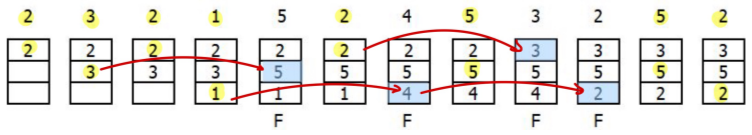
\includegraphics[width=0.8\linewidth]{page_replacement_SEP19.png}
\end{example2}





\subsection{Virtual Memory Addressing}

\begin{KR}{Virtual Memory Address Analysis}
    \paragraph{Address structure calculation}
    \begin{itemize}
        \item Page offset bits = $log_2$(page size in bytes)
        \item Remaining bits = total address bits - offset bits
        \item Bits per level = remaining bits ÷ number of levels
    \end{itemize}
    
    \paragraph{Page table size calculation}
    \begin{itemize}
        \item Entries per table = 2\textsuperscript{bits per level}
        \item Table size = entries × entry size in bytes
        \item Number of tables per level = cumulative from higher levels
    \end{itemize}
    
    \paragraph{Common mistakes to avoid}
    \begin{itemize}
        \item Forgetting to account for page offset bits
        \item Mixing up table levels in size calculations
        \item Not considering that tables should fit in pages
    \end{itemize}
\end{KR}

\begin{example2}{Virtual Memory Address Translation}
    Given: 16KB page size, 47-bit virtual addresses, 3-level paging, 8-byte page table entries.
    
    How is a virtual address structured?
    
    \tcblower
    
    \textbf{Calculation:}
    \begin{itemize}
        \item Page size: 16KB = 2\textsuperscript{14} bytes $\rightarrow$ 14 bits for page offset
        \item Remaining bits: 47 - 14 = 33 bits for page table indexing
        \item 3 levels: 33 ÷ 3 = 11 bits per page table level
    \end{itemize}
    
    \textbf{Address structure:}
    \begin{tabular}{|c|c|c|c|}
        \hline
        Bits 46-36 & Bits 35-25 & Bits 24-14 & Bits 13-0 \\
        \hline
        Level 1 (11 bit) & Level 2 (11 bit) & Level 3 (11 bit) & Offset (14 bit) \\
        \hline
    \end{tabular}
    
    \textbf{Page table sizes:}
    \begin{itemize}
        \item Level 1: 1 table with 2\textsuperscript{11} = 2048 entries
        \item Level 2: 2048 tables with 2048 entries each
        \item Level 3: 2048\textsuperscript{2} = 4,194,304 tables with 2048 entries each
        \item Each table: 2048 × 8 bytes = 16KB (exactly one page)
    \end{itemize}
\end{example2}

\important{ADD EXERCISE 12 SEP07 SEGMENTATION}

\raggedcolumns
\pagebreak

\subsection{Memory Management Analysis}

\mult{2}

\begin{formula}{Buddy System}
    \begin{itemize}
        \item Alloziert in Potenzen von 2 (1, 2, 4, 8, 16, ... KByte)
        \item Interne Fragmentierung = Alloziert - Angefordert
        \item Nächste grössere 2er-Potenz finden: 2\textsuperscript{n} $\geq$ Anforderung
        \item Beispiel: 33 KByte $\rightarrow$ 64 KByte (2\textsuperscript{6})
    \end{itemize}
\end{formula}

\begin{formula}{Page Table Berechnung}
    \begin{itemize}
        \item Page-Grösse = 2\textsuperscript{Offset-Bits} Bytes
        \item Anzahl Pages = 2\textsuperscript{Page-Number-Bits}
        \item Page Directory Grösse = 2\textsuperscript{Directory-Bits} × Pointer-Grösse
        \item Maximale Frames = 2\textsuperscript{(Physische-Adress-Bits - Offset-Bits)}
    \end{itemize}
\end{formula}

\begin{formula}{Addressaufteilung}
    \begin{itemize}
        \item Logische Adresse = Page Directory + Page Number + Offset
        \item Physische Adresse = Frame Number + Offset
        \item Page Table Entry enthält Frame Number
        \item Translation: Page Number $\rightarrow$ Frame Number
    \end{itemize}
\end{formula}

\begin{concept}{Memory Hierarchy}
    \begin{itemize}
        \item Page Directory zeigt auf Page Tables
        \item Page Tables zeigen auf Frames
        \item Mehrstufige Page Tables reduzieren Speicherbedarf
        \item TLB cached häufig verwendete Translations
    \end{itemize}
\end{concept}

\multend

\subsubsection{Memory Access Time Calculation}


\begin{KR}{Average Memory Access Time}
    
    \paragraph{Calculation method}
    \begin{itemize}
        \item Start from L1 cache (always accessed first)
        \item Apply formula from innermost level outward
        \item For each miss, calculate probability of accessing next level (e.g. L3 miss probability = $(1-h_1) \times (1-h_2) \times (1-h_3)$)
        \item Multiply access time by probability of reaching that level
        \item Sum all weighted access times
    \end{itemize}
    
    \paragraph{Formula}
    \begin{itemize}
        \item $T_{avg} = T_{L1} + (1-h_1) \times T_{L2} + (1-h_1)(1-h_2) \times T_{L3} + \ldots$
        \item Convert clock cycles to nanoseconds: Time = Cycles $\times$ Clock period (or Cycle time)
        \item Clock period = 1 / Frequency
    \end{itemize}
\end{KR}

\begin{example2}{Memory Access Time Calculation}
    2 GHz processor (0.5 ns cycle), 90\% hit rate on all levels:
    
    \begin{tabular}{|l|l|}
        \hline
        L1 Cache & 4 cycles = 2.0 ns \\
        L2 Cache & 10 cycles = 5.0 ns \\
        L3 Cache & 40 cycles = 20.0 ns \\
        Main Memory & 60 ns \\
        \hline
    \end{tabular}
    
    \tcblower
    
    \textbf{Calculation:}
    \begin{itemize}
        \item L1 access: $4 \times 0.5 = 2$ ns (always accessed)
        \item L2 access: $10 \times 0.5 = 5$ ns (10\% probability)
        \item L3 access: $40 \times 0.5 = 20$ ns (1\% probability)  
        \item Main memory: 60 ns (0.1\% probability)
        \item $T_{avg} = 2 + 0.1 \times 5 + 0.01 \times 20 + 0.001 \times 60$
        \item $T_{avg} = 2 + 0.5 + 0.2 + 0.06 = 2.76$ ns
    \end{itemize}
\end{example2}

\subsubsection{Cache Performance Analysis}

\important{TODO: add theory and example!!}

\begin{KR}{Cache Hit Rate Calculation}
    \paragraph{Problem identification}
    \begin{itemize}
        \item Given: Array access pattern, processor architecture, cache block size
        \item Find: Cache hit rate during sequential array access
    \end{itemize}

    \paragraph{Given information analysis}
    \begin{itemize}
        \item Identify data type size (e.g., int = 4 bytes on 32-bit system)
        \item Note cache line size (e.g., 64 bytes)
        \item Determine access pattern (sequential vs. random)
    \end{itemize}
    
    \paragraph{Solution approach}
    \begin{itemize}
        \item Calculate element (data type) size based on processor architecture
        \item Determine how many array elements fit in one cache line
        \item For sequential access: First access to cache line = miss, rest = hits
    \end{itemize}
    
    \paragraph{Key formulas}
    \begin{itemize}
        \item Elements per cache line = Cache line size / Element size
        \item Hit rate = Number of hits / Total accesses
        \item For 32-bit processor: int = 4 bytes
        \item For 64-bit processor: int = 4 bytes, long = 8 bytes
    \end{itemize}
\end{KR}

\begin{example2}{Cache Access Analysis}
    Given code accessing an integer array sequentially:
    
\begin{lstlisting}[language=C, style=basesmol]
#define N (10*1000*1000)
int arVL[N];
for (int i = 0; i < N; i++) {
    sum += arVL[i];
}
\end{lstlisting}

Calculate hit rate on a 32-bit processor with 64-byte cache lines.

    \tcblower
    
    \textbf{Analysis:}
    \begin{itemize}
        \item 32-bit system (processor): int = 4 bytes
        \item Cache line size: 64 bytes
        \item Elements per cache line: 64/4 = 16 integers
        \item Access pattern: Sequential $\rightarrow$ first access per line: cache miss
        \item For every 16 accesses: 1 miss + 15 hits
        \item Hit rate: $h_c$ = 15/16 = 0.9375 = 93.75\%
    \end{itemize}
\end{example2}

\raggedcolumns
\pagebreak

\subsection{Linux Memory Management}

\mult{2}

\begin{definition}{Linux Page Table Organization}\\
    Linux uses a hierarchical page table structure:
    \begin{itemize}
        \item Multi-level page directory to reduce size and improve lookup speed
        \item Typically 4-level structure:
            \begin{itemize}
                \item Page Global Directory (PGD)
                \item Page Upper Directory (PUD)
                \item Page Middle Directory (PMD)
                \item Page Table Entry (PTE)
            \end{itemize}
        \item Allows efficient handling of sparse address spaces
        \item Only allocates page tables for used parts of address space
    \end{itemize}
\end{definition}

\begin{definition}{Huge Pages} supported to improve performance:
    \begin{itemize}
        \item Standard page size is 4KB
        \item Huge pages can be 2MB or 1GB \\(architecture-dependent)
        \item Advantages:
            \begin{itemize}
                \item Reduces TLB pressure (fewer entries needed to cover same memory)
                \item Improves performance for memory-intensive applications
                \item More efficient for large memory allocations
            \end{itemize}
        \item Uses higher-level page table entries (PUD/PMD)
        \item Requires explicit configuration
    \end{itemize}
\end{definition}

\multend

\begin{concept}{Memory Zones}\\
    Linux divides physical memory into zones to handle hardware limitations:
    \begin{itemize}
        \item \textbf{ZONE\_DMA}: Memory addressable by DMA controllers (typically below 16MB)
        \item \textbf{ZONE\_NORMAL}: Regularly mapped memory in kernel space
        \item \textbf{ZONE\_HIGHMEM}: Memory beyond what the kernel can directly address
        \item Zones are managed separately to accommodate different hardware constraints
        \item Each zone has its own free lists and allocation policies
    \end{itemize}
\end{concept}

\begin{theorem}{Buddy Allocator}
    Linux uses the buddy system for frame allocation:
    \begin{itemize}
        \item Fundamental allocation unit is the page frame
        \item Maintains lists of free blocks of various sizes (powers of 2)
        \item When a process requests memory:
            \begin{itemize}
                \item System finds the smallest block size that fits the request
                \item If necessary, splits larger blocks into "buddies"
                \item Allocates memory from appropriate free list
            \end{itemize}
        \item When memory is freed:
            \begin{itemize}
                \item System checks if buddy is also free
                \item If so, merges buddies to form larger block
                \item Continues merging recursively if possible
            \end{itemize}
        \item Maintains free lists up to MAX\_ORDER-1 (typically 10, so up to 512 contiguous pages)
    \end{itemize}
\end{theorem}

\begin{theorem}{Slab Allocator}
    Linux uses the slab allocator for kernel objects:
    \begin{itemize}
        \item Kernel often requires small allocations for data structures
        \item Pages (4KB) are too large for many kernel objects
        \item Slab allocator:
            \begin{itemize}
                \item Gets pages from buddy allocator
                \item Divides them into smaller objects of specific types
                \item Maintains caches of frequently used object types
                \item Reuses recently freed objects (helps prevent fragmentation)
                \item Preserves object state between uses
            \end{itemize}
        \item Improves memory utilization and allocation speed
        \item Minimizes internal fragmentation
    \end{itemize}
\end{theorem}

\begin{formula}{Memory Compaction}
    Linux performs memory compaction to address fragmentation:
    \begin{itemize}
        \item Problem: Buddy allocator may not find large contiguous blocks
        \item Solution: kcompactd daemon performs compaction
        \item Process:
            \begin{itemize}
                \item Balances memory zones by swapping out non-working-set pages
                \item Moves movable pages toward the top of the memory zone
                \item Leaves bottom of memory free for new allocations
                \item Creates larger contiguous free blocks
            \end{itemize}
        \item Performed on-demand or periodically
        \item Enables allocation of huge pages and other large memory blocks
    \end{itemize}
\end{formula}

\begin{formula}{Shared Libraries}
    Linux uses shared libraries to reduce memory usage:
    \begin{itemize}
        \item Multiple processes can use the same library code
        \item Libraries compiled with -fPIC (Position Independent Code)
        \item Dynamically linked with processes using ld.so
        \item Read-only code pages memory-mapped into processes
        \item Benefits:
            \begin{itemize}
                \item Reduces memory footprint
                \item Shared code/text pages only loaded once
                \item Only data pages need to be process-specific
            \end{itemize}
        \item Challenge: Version compatibility ("DLL hell")
    \end{itemize}
\end{formula}

\begin{formula}{Page Reclamation}
    Linux uses page reclamation to recover memory:
    \begin{itemize}
        \item Working set: Pages actively in use by processes
        \item Resident set: All pages in memory
        \item A page is in the working set if:
            \begin{itemize}
                \item Accessed via process address space
                \item Accessed via system call
                \item Accessed via device driver
            \end{itemize}
        \item Linux identifies non-working set pages using a bitmap
        \item Pages marked idle can be reclaimed when memory is needed
    \end{itemize}
\end{formula}

\begin{formula}{Least Recently Used in Linux}\\
    Linux implements a two-stage LRU algorithm:
    \begin{itemize}
        \item Maintains two lists of page frames:
            \begin{itemize}
                \item Active list: Recently accessed pages
                \item Inactive list: Less recently accessed pages
            \end{itemize}
        \item Pages move between lists based on access patterns
        \item Inactive pages are candidates for reclamation
        \item Recently accessed inactive pages can be promoted to active list
        \item Linux uses a global strategy for page reclamation
        \item Recent development: Multi-Generational LRU (MGLRU)
            \begin{itemize}
                \item Assigns generation numbers to page frames based on recent access
                \item Older generations are reclaimed first
                \item Improves performance and responsiveness
            \end{itemize}
    \end{itemize}
\end{formula}

\begin{theorem}{Out-of-Memory (OOM) Killer}
    Linux has an OOM Killer to handle critical memory shortages:
    \begin{itemize}
        \item Activates when system is critically low on memory
        \item Linux tends to be optimistic in memory allocation
            \begin{itemize}
                \item Processes typically request more memory than needed
                \item System may over-allocate (more than physical memory)
            \end{itemize}
        \item OOM Killer selects processes to terminate based on heuristics
            \begin{itemize}
                \item Considers memory usage, runtime, nice value, etc.
                \item Each process has an oom\_score in /proc/\$PID/oom\_score
                \item Can be adjusted through oom\_score\_adj
            \end{itemize}
        \item Prioritizes system stability over individual process survival
    \end{itemize}
\end{theorem}

\begin{KR}{Memory Management Analysis in Linux}
    \paragraph{Basic memory information}
    \begin{itemize}
        \item Display system memory usage: \texttt{free -h}
        \item View memory details: \texttt{cat /proc/meminfo}
        \item Check process memory usage: \texttt{ps -eo pid,ppid,cmd,vsz,rss}
        \item Interactive memory monitor: \texttt{top} or \texttt{htop}
    \end{itemize}
    
    \paragraph{Process memory analysis}
    \begin{itemize}
        \item Check process memory maps: \texttt{cat /proc/\$PID/maps}
        \item View process memory status: \texttt{cat /proc/\$PID/status}
        \item Analyze memory usage in detail: \texttt{pmap \$PID}
        \item Track memory over time: \texttt{smem}
    \end{itemize}
    
    \paragraph{Memory page information}
    \begin{itemize}
        \item Get page size: \texttt{getconf PAGE\_SIZE}
        \item Check huge pages: \texttt{cat /proc/meminfo | grep Huge}
        \item View page stats: \texttt{cat /proc/pagetypeinfo}
        \item Check page faults: \texttt{ps -o min\_flt,maj\_flt \$PID}
    \end{itemize}
    
    \paragraph{Memory limits and control}
    \begin{itemize}
        \item Set memory limits: \texttt{ulimit -m [size]}
        \item Control cgroup memory: \texttt{echo [value] > /sys/fs/cgroup/memory/[group]/memory.limit\_in\_bytes}
        \item Check swappiness: \texttt{cat /proc/sys/vm/swappiness}
        \item Adjust swappiness: \texttt{sysctl vm.swappiness=[value]}
    \end{itemize}
\end{KR}

\begin{example2}{Analyzing Process Memory}
    Check memory usage details for a process:
    
\begin{lstlisting}[language=bash, style=basesmol]
# Get PID of a process
PID=$(pidof firefox)

# Check virtual and resident memory size
ps -o pid,comm,vsz,rss -p $PID

# Analyze memory map segments
cat /proc/$PID/maps | head -10

# View detailed memory status
grep -E 'VmSize|VmRSS|VmData|VmStk|VmExe' /proc/$PID/status

# Map process address space in detail
pmap -x $PID | head -20

# Check page faults
ps -o min_flt,maj_flt -p $PID
\end{lstlisting}

    \tcblower
    
    \textbf{Explanation of memory terms:}
    \begin{itemize}
        \item \textbf{VSZ (Virtual Size)}: Total virtual memory allocated to process
        \item \textbf{RSS (Resident Set Size)}: Actual physical memory used
        \item \textbf{VmData}: Size of data segment
        \item \textbf{VmStk}: Size of stack
        \item \textbf{VmExe}: Size of text segment
        \item \textbf{min\_flt}: Minor page faults (page in memory but not in process's page table)
        \item \textbf{maj\_flt}: Major page faults (page had to be loaded from disk)
    \end{itemize}
\end{example2}

\begin{example2}{Working with Page Size and Memory Allocation}
    Analyzing page size and memory allocation:
    
\begin{lstlisting}[language=C, style=basesmol]
#include <stdio.h>
#include <stdlib.h>
#include <unistd.h>
#include <sys/mman.h>

int main() {
    // Get process ID
    pid_t pid = getpid();
    printf("Process ID: %d\n", pid);
    
    // Get page size
    int page_size = getpagesize();
    printf("Page size: %d bytes\n", page_size);
    
    // Allocate memory for 10 pages
    size_t size = 10 * page_size;
    char *buffer = malloc(size);
    printf("Allocated %zu bytes (%zu pages)\n", 
           size, size / page_size);
    
    // Check page faults before access
    printf("Check page faults with: ps -o min_flt,maj_flt %d\n", pid);
    printf("Press Enter to continue...\n");
    getchar();
    
    // Access the memory (causes page faults)
    for (int i = 0; i < size; i += page_size) {
        buffer[i] = 1;  // Touch one byte per page
    }
    
    // Check page faults after access
    printf("Check page faults again with: ps -o min_flt,maj_flt %d\n", pid);
    printf("Press Enter to continue...\n");
    getchar();
    
    // Allocate page-aligned memory
    void *aligned_buf = NULL;
    int result = posix_memalign(&aligned_buf, page_size, size);
    if (result == 0) {
        printf("Allocated %zu bytes aligned on page boundary\n", size);
    }
    
    // Free memory
    free(buffer);
    free(aligned_buf);
    
    return 0;
}
\end{lstlisting}

    This example demonstrates:
    \begin{itemize}
        \item Getting the system page size
        \item Allocating memory
        \item Observing page faults due to lazy allocation
        \item Creating page-aligned memory allocations
    \end{itemize}
\end{example2}


	\raggedcolumns
	\pagebreak
	\section{Input / Output - Part I}

\subsection{Input/Output Basics}

\begin{concept}{I/O Challenges}\\
    I/O management presents unique challenges for operating systems:
    \begin{itemize}
        \item Huge variety of I/O devices (keyboards, mice, drives, sensors, etc.)
        \item Diverse interfaces (ATA, SATA, USB, PCI, etc.)
        \item Wide range of speeds and capacities
        \item Different data transfer characteristics
        \item Need for a unified approach to device interaction
    \end{itemize}
    
    The operating system must abstract this heterogeneity by providing consistent interfaces for applications to access diverse devices.
\end{concept}

\begin{definition}{Device Categories}\\
    From a user perspective, devices fall into two main categories:
    \begin{itemize}
        \item \textbf{Block Devices}:
            \begin{itemize}
                \item Operate on fixed-size blocks of data
                \item Support random access to any block
                \item Example: Hard drives, SSDs
                \item Block operations are independent from each other
                \item Block size defined when formatting (logical)
                \item Sector size is the physical unit on the device
            \end{itemize}
        \item \textbf{Character Devices}:
            \begin{itemize}
                \item Operate on streams of characters
                \item Generally sequential access
                \item Example: Keyboards, mice, printers
                \item Characters are interpretations of bit patterns according to specifications (ASCII, Unicode)
                \item Character devices ultimately operate on bit-level too
            \end{itemize}
    \end{itemize}
\end{definition}

\subsection{I/O Hardware Architecture}

\begin{definition}{I/O Hardware Components}\\
    Key components in I/O hardware architecture:
    \begin{itemize}
        \item \textbf{I/O Controller}: Electronic interface to the device
            \begin{itemize}
                \item Typically one per device category (SCSI, IDE, USB, Ethernet)
                \item Contains registers that control device operation
                \item Maintains buffers for read/write operations
                \item Communicates with CPU and main memory
            \end{itemize}
        \item \textbf{I/O Ports}: Addresses that point to controller registers
        \item \textbf{Buffers}: Memory areas for data transfer
        \item \textbf{Bus System}: Connects CPU, memory, and I/O devices
    \end{itemize}
\end{definition}

\begin{definition}{I/O Address Space}\\
    X86 architecture has two approaches for I/O address allocation:
    \begin{itemize}
        \item \textbf{Port Mapped I/O (PMIO)}:
            \begin{itemize}
                \item Peripheral I/O registers assigned to a dedicated address range
                \item Distinct from system memory
                \item Uses dedicated I/O instructions (IN and OUT)
                \item Limited to 64K ports (16-bit addressing)
                \item Common for older peripherals (e.g., ISA cards)
                \item Listed in \texttt{/proc/ioports}
            \end{itemize}
        \item \textbf{Memory Mapped I/O (MMIO)}:
            \begin{itemize}
                \item Peripheral registers mapped into main memory address space
                \item Uses regular memory instructions (e.g., MOV)
                \item Default in modern systems (e.g., PCIe, PCI)
                \item Listed in \texttt{/proc/iomem}
            \end{itemize}
    \end{itemize}
\end{definition}

\begin{definition}{Direct Memory Access (DMA)}\\
    DMA improves I/O performance:
    \begin{itemize}
        \item Allows devices to transfer data directly to/from memory
        \item Bypasses CPU for bulk data transfer
        \item CPU sets up transfer parameters:
            \begin{itemize}
                \item Memory address
                \item Count of bytes to transfer
                \item Direction (read/write)
                \item Device-specific parameters
            \end{itemize}
        \item DMA controller handles the actual transfer
        \item Interrupts CPU when transfer completes
        \item Reduces CPU overhead for data-intensive I/O operations
    \end{itemize}
\end{definition}

\subsection{I/O Principles}

\begin{definition}{I/O Access Methods}\\
    Two primary methods for CPU to interact with I/O devices:
    \begin{itemize}
        \item \textbf{Programmed I/O}:
            \begin{itemize}
                \item CPU does all the work
                \item CPU executes instructions to transfer data
                \item CPU repeatedly checks device status (polling/busy-waiting)
                \item Synchronous operation (CPU waits for I/O completion)
                \item Simple but inefficient for slow devices
            \end{itemize}
        \item \textbf{Interrupt-driven I/O}:
            \begin{itemize}
                \item Devices signal CPU when they need attention
                \item CPU initiates operation then continues other work
                \item Device interrupts when operation completes
                \item Asynchronous operation
                \item More efficient, especially for slow devices
            \end{itemize}
    \end{itemize}
\end{definition}

\begin{definition}{Interrupt Handling}\\
    Interrupts are fundamental to efficient I/O:
    \begin{itemize}
        \item \textbf{Interrupt}: Event that defers the normal flow of CPU execution
        \item When an interrupt occurs:
            \begin{itemize}
                \item Current execution is suspended
                \item CPU state is saved
                \item Special routine (interrupt handler) is executed
                \item After completion, previous execution resumes
            \end{itemize}
        \item \textbf{Interrupt types}:
            \begin{itemize}
                \item \textbf{Synchronous}: Generated by executing an instruction (e.g., divide by zero)
                \item \textbf{Asynchronous}: Generated by external events (e.g., I/O completion)
            \end{itemize}
        \item \textbf{Interrupt classifications}:
            \begin{itemize}
                \item \textbf{Maskable}: Can be ignored by setting interrupt mask
                \item \textbf{Non-maskable}: Cannot be ignored (critical events)
            \end{itemize}
    \end{itemize}
\end{definition}

\begin{definition}{Interrupt Flow}\\
    Hardware interrupt flow:
    \begin{itemize}
        \item Device raises interrupt on its IRQ line
        \item Programmable Interrupt Controller (PIC) converts IRQ to vector number
        \item PIC signals CPU via INTR pin
        \item CPU acknowledges interrupt
        \item CPU executes the appropriate interrupt handler
        \item In Linux, interrupt handling occurs in three phases:
            \begin{itemize}
                \item Critical: Minimal processing, acknowledge interrupt
                \item Immediate: Essential processing, can't be deferred
                \item Deferred: Non-critical processing, scheduled for later
            \end{itemize}
    \end{itemize}
\end{definition}

\begin{definition}{I/O Access Patterns}\\
    Different access patterns affect I/O performance:
    \begin{itemize}
        \item \textbf{Exclusive vs. Shared Access}:
            \begin{itemize}
                \item Exclusive: Device dedicated to one process
                \item Shared: Multiple processes access same device
                \item Shared access requires scheduling (e.g., disk I/O scheduling)
            \end{itemize}
        \item \textbf{Sequential vs. Random Access}:
            \begin{itemize}
                \item Sequential: Data accessed in order (e.g., tape)
                \item Random: Data accessed in any order (e.g., disk)
            \end{itemize}
        \item \textbf{Blocking vs. Non-Blocking}:
            \begin{itemize}
                \item Blocking: Process waits until I/O completes
                \item Non-Blocking: Process continues, checks completion later
            \end{itemize}
        \item \textbf{Synchronous vs. Asynchronous}:
            \begin{itemize}
                \item Synchronous: Process execution synchronized with I/O completion
                \item Asynchronous: Process continues, notified of I/O completion
            \end{itemize}
    \end{itemize}
\end{definition}

\begin{definition}{Buffered vs. Direct I/O}\\
    Buffering improves I/O performance:
    \begin{itemize}
        \item \textbf{Buffered I/O}:
            \begin{itemize}
                \item Data passes through intermediate buffer
                \item Decouples data access from data generation
                \item Handles different speeds between devices
                \item Enables rate control
                \item Allows data manipulation before final transfer
                \item Supports data verification
            \end{itemize}
        \item \textbf{Direct I/O}:
            \begin{itemize}
                \item Data transferred directly to/from device
                \item Bypasses system caches
                \item Reduces memory usage and CPU overhead
                \item Useful for applications with their own caching
                \item May be slower for some workloads
            \end{itemize}
    \end{itemize}
\end{definition}

\begin{definition}{Error Handling}\\
    I/O systems must handle errors effectively:
    \begin{itemize}
        \item Errors can occur at various levels:
            \begin{itemize}
                \item Bit-level, byte-level, packet-level, block-level
                \item Hardware vs. software detection
                \item User space vs. kernel space handling
            \end{itemize}
        \item Error handling approaches:
            \begin{itemize}
                \item Error Detection: Identify errors (e.g., checksums, parity)
                \item Error Correction: Fix errors without retransmission
                \item Error Recovery: Return to consistent state after error
            \end{itemize}
        \item Trade-offs between performance and reliability
    \end{itemize}
\end{definition}

\subsection{Linux I/O Subsystem}

\begin{definition}{Linux Device Model}\\
    The Linux Device Model maintains the state and structure of the system:
    \begin{itemize}
        \item Maintains information about devices, drivers, buses, etc.
        \item Key entities:
            \begin{itemize}
                \item \textbf{Device}: Physical device attached to a bus
                \item \textbf{Driver}: Software entity that operates devices
                \item \textbf{Bus}: Device to which other devices can be attached
                \item \textbf{Class}: Type of device with similar behavior
                \item \textbf{Subsystem}: View on the system structure
            \end{itemize}
        \item Represented in user space via sysfs (mounted at /sys)
    \end{itemize}
\end{definition}

\begin{definition}{sysfs}\\
    sysfs is a virtual filesystem that exposes the Linux Device Model:
    \begin{itemize}
        \item Located at /sys
        \item Key directories:
            \begin{itemize}
                \item \texttt{/sys/block}: Block devices
                \item \texttt{/sys/bus}: Bus types
                \item \texttt{/sys/class}: Device classes
                \item \texttt{/sys/devices}: Hierarchical device structure
                \item \texttt{/sys/firmware}: Firmware information
                \item \texttt{/sys/fs}: Filesystem information
                \item \texttt{/sys/kernel}: Kernel status
                \item \texttt{/sys/module}: Loaded modules
                \item \texttt{/sys/power}: Power management
            \end{itemize}
        \item Contains attributes in files for configuration and status
    \end{itemize}
\end{definition}

\begin{definition}{udev}\\
    udev is the userspace device manager for Linux:
    \begin{itemize}
        \item Part of systemd
        \item systemd-udevd listens to kernel events
        \item Executes rules based on device information from sysfs
        \item Creates or removes device nodes in /dev
        \item Provides consistent device naming
        \item Enables automatic device setup
        \item Supports user-defined rules
    \end{itemize}
\end{definition}

\begin{definition}{/dev Directory}\\
    The /dev directory contains special files representing devices:
    \begin{itemize}
        \item Each file represents an I/O device
        \item Allows standard file operations (open, read, write, close) on devices
        \item When accessed, kernel routes operations to appropriate device drivers
        \item Types of device files:
            \begin{itemize}
                \item Character device files: For character devices
                \item Block device files: For block devices
            \end{itemize}
        \item Naming conventions:
            \begin{itemize}
                \item \texttt{/dev/sdX}: SCSI/SATA disk devices
                \item \texttt{/dev/ttyX}: Terminal devices
                \item \texttt{/dev/nullX}: Special device files
            \end{itemize}
    \end{itemize}
\end{definition}

\begin{definition}{Device Access in Linux}\\
    Linux provides a unified interface for device access:
    \begin{itemize}
        \item Applications use standard file operations:
            \begin{itemize}
                \item \texttt{open()}: Open device
                \item \texttt{read()}: Read from device
                \item \texttt{write()}: Write to device
                \item \texttt{ioctl()}: Device-specific operations
                \item \texttt{close()}: Close device
            \end{itemize}
        \item Kernel translates these operations to device-specific commands
        \item Virtual File System (VFS) provides abstraction layer
        \item Device drivers implement the specific operations
    \end{itemize}
\end{definition}

\begin{KR}{Working with I/O in Linux}\\
    \paragraph{Exploring device information}
    \begin{itemize}
        \item List I/O ports: \texttt{cat /proc/ioports}
        \item List I/O memory: \texttt{cat /proc/iomem}
        \item View interrupts: \texttt{cat /proc/interrupts}
        \item List block devices: \texttt{lsblk}
        \item Show hardware: \texttt{lshw}
        \item Display PCI devices: \texttt{lspci}
        \item List USB devices: \texttt{lsusb}
    \end{itemize}
    
    \paragraph{Working with devices}
    \begin{itemize}
        \item Check device information: \texttt{udevadm info --query=all --name=/dev/sda}
        \item Monitor device events: \texttt{udevadm monitor}
        \item Show device properties: \texttt{udevadm info --attribute-walk --name=/dev/sda}
        \item Check I/O performance: \texttt{iostat -x}
        \item Monitor I/O activity: \texttt{iotop}
    \end{itemize}
    
    \paragraph{Device file operations}
    \begin{itemize}
        \item Create device file: \texttt{mknod /dev/example c 1 3}
        \item Read from device: \texttt{cat /dev/input/mouse0 | hexdump}
        \item Write to device: \texttt{echo "test" > /dev/tty1}
        \item Control device: \texttt{ioctl} system call in C programs
    \end{itemize}
\end{KR}

\begin{example2}{I/O Performance Testing}\\
    Testing disk write performance with different options:
    
\begin{lstlisting}[language=bash, style=basesmol]
# Basic write test (with caching)
dd if=/dev/zero of=speedtest bs=10M count=100
rm speedtest

# Write test with synchronous I/O (forces data to disk)
dd if=/dev/zero of=speedtest bs=10M count=100 conv=fdatasync
rm speedtest

# Write test with direct I/O (bypasses the page cache)
dd if=/dev/zero of=speedtest bs=10M count=100 oflag=direct
rm speedtest

# Monitor disk I/O activity during test
iostat -x 1

# Check disk utilization statistics
iostat -p sda

# Explanation:
# - Standard dd shows high performance but may not be on disk yet
# - fdatasync ensures data is physically written to disk
# - direct bypasses the OS cache, showing raw device performance
\end{lstlisting}
\end{example2}

\begin{example2}{Device Information Analysis}\\
    Exploring device information in Linux:
    
\begin{lstlisting}[language=bash, style=basesmol]
# List block devices with details
lsblk -f

# Get detailed information about a specific device
udevadm info --query=all --name=/dev/sda1

# Examine sysfs entries for the device
ls -l /sys/block/sda/sda1/

# Check device attributes
cat /sys/block/sda/queue/scheduler
cat /sys/block/sda/queue/read_ahead_kb

# Get PCI information for a disk controller
lspci | grep -i sata

# Check all properties of a device
udevadm info --attribute-walk --name=/dev/sda1 | less

# Monitor udev events when plugging in a USB device
udevadm monitor --property
# (Now plug in a USB device to see events)
\end{lstlisting}
\end{example2}
	\raggedcolumns
	\pagebreak
	\section{Input / Output - Part II}

\subsection{Building and Using a Custom Linux Kernel}

\begin{concept}{Custom Kernel Motivation}\\
    There are various reasons to build a custom kernel:
    \begin{itemize}
        \item Create a minimalist kernel (disable unused features, load needed ones as modules)
        \item Add custom OS features for specific requirements
        \item Support special hardware that may not be in the standard kernel
        \item Optimize for specific workloads or hardware platforms
        \item Learn about kernel internals and development processes
    \end{itemize}
\end{concept}

\begin{definition}{Linux Kernel Development Process}\\
    Linux follows a time-based release process:
    \begin{itemize}
        \item New major kernel releases every 2-3 months (e.g., 5.11, 5.12)
        \item Development cycle phases:
            \begin{itemize}
                \item Merge window (first two weeks): New features merged into mainline
                \item Release candidates (weekly): Bug fixes only, no new features
                \item Final release: After several release candidates
            \end{itemize}
        \item Long-term support (LTS) kernels receive updates for extended periods
        \item Community development model with maintainers for various subsystems
    \end{itemize}
\end{definition}

\begin{definition}{Choosing a Kernel Version}\\
    When building a custom kernel, version selection matters:
    \begin{itemize}
        \item Mainline: Latest development version (might be unstable)
        \item Stable: Recent release with proven stability
        \item Long-term: Longer support period (good for production systems)
        \item Distribution-specific: Modified by Linux distributions
    \end{itemize}
    
    Version numbers indicate:
    \begin{itemize}
        \item First number: Major version (rarely changes)
        \item Second number: Minor version (major features)
        \item Third number: Patch level (bug fixes and minor improvements)
    \end{itemize}
\end{definition}

\begin{KR}{Building a Custom Linux Kernel}\\
    \paragraph{Getting the source code}
    \begin{itemize}
        \item Download from kernel.org: \texttt{wget https://cdn.kernel.org/pub/linux/kernel/v5.x/linux-5.xx.tar.xz}
        \item Extract: \texttt{tar xf linux-5.xx.tar.xz}
        \item Change directory: \texttt{cd linux-5.xx}
    \end{itemize}
    
    \paragraph{Installing build dependencies}
    \begin{itemize}
        \item On Debian/Ubuntu: \texttt{sudo apt-get install build-essential gcc bc bison flex libssl-dev libncurses5-dev libelf-dev}
    \end{itemize}
    
    \paragraph{Configuring the kernel}
    \begin{itemize}
        \item Start from existing config (recommended):
            \begin{itemize}
                \item Current running kernel: \texttt{cp /boot/config-\$(uname -r) ./.config}
                \item Distribution default: \texttt{make defconfig}
            \end{itemize}
        \item Update config for new options: \texttt{make oldconfig}
        \item Interactive configuration tools:
            \begin{itemize}
                \item Text-based menu: \texttt{make menuconfig}
                \item GUI-based: \texttt{make xconfig} or \texttt{make gconfig}
            \end{itemize}
        \item Important configuration options:
            \begin{itemize}
                \item Custom version name: \texttt{CONFIG\_LOCALVERSION}
                \item Module support: \texttt{CONFIG\_MODULES}
                \item CPU and architecture options
                \item Device drivers
                \item File systems
            \end{itemize}
    \end{itemize}
    
    \paragraph{Building the kernel}
    \begin{itemize}
        \item Compile: \texttt{make -j\$(nproc)}
        \item Build modules: \texttt{make modules}
        \item Create Debian/Ubuntu packages: \texttt{make -j\$(nproc) deb-pkg}
        \item For RPM-based systems: \texttt{make -j\$(nproc) rpm-pkg}
    \end{itemize}
    
    \paragraph{Installing the kernel}
    \begin{itemize}
        \item Debian packages: \texttt{sudo dpkg -i ../linux-*.deb}
        \item RPM packages: \texttt{sudo rpm -ivh ../linux-*.rpm}
        \item Manual installation:
            \begin{itemize}
                \item Install modules: \texttt{sudo make modules\_install}
                \item Install kernel: \texttt{sudo make install}
            \end{itemize}
        \item Update bootloader: \texttt{sudo update-grub} (GRUB)
    \end{itemize}
    
    \paragraph{Booting the new kernel}
    \begin{itemize}
        \item Reboot: \texttt{sudo reboot}
        \item Select the new kernel at the bootloader menu
        \item Verify running kernel: \texttt{uname -a}
    \end{itemize}
\end{KR}

\subsection{Linux Kernel Modules}

\begin{definition}{Kernel Modules Concept}\\
    Kernel modules extend kernel functionality without rebuilding:
    \begin{itemize}
        \item Loadable code that can be added to or removed from a running kernel
        \item Allow dynamic extension of kernel capabilities
        \item Provide device drivers, filesystem drivers, system calls, etc.
        \item Reduce the size of the base kernel
        \item Enable support for hardware that is hot-pluggable
        \item Support for special features used in specific applications
    \end{itemize}
\end{definition}

\begin{definition}{Module Structure}\\
    A kernel module follows a specific structure:
    \begin{itemize}
        \item Must include necessary kernel headers
        \item Initialization function (\texttt{init\_module()} or custom named)
            \begin{itemize}
                \item Called when the module is loaded
                \item Sets up resources, registers with kernel subsystems
                \item Returns success (0) or error code
            \end{itemize}
        \item Cleanup function (\texttt{cleanup\_module()} or custom named)
            \begin{itemize}
                \item Called when the module is unloaded
                \item Releases resources, unregisters from kernel subsystems
            \end{itemize}
        \item Uses \texttt{MODULE\_LICENSE()} macro to specify license
        \item Can include other macros for author, description, etc.
    \end{itemize}
\end{definition}

\begin{code}{Hello World Kernel Module}\\
    Minimal kernel module example:
    
\begin{lstlisting}[language=C, style=basesmol]
#include <linux/module.h>    /* Needed by all modules */
#include <linux/kernel.h>    /* Needed for KERN_INFO */
#include <linux/init.h>      /* Needed for macros */

MODULE_LICENSE("GPL");
MODULE_AUTHOR("Your Name");
MODULE_DESCRIPTION("A simple Hello World module");

static int __init hello_init(void)
{
    printk(KERN_INFO "Hello, World!\n");
    return 0;    /* Success */
}

static void __exit hello_exit(void)
{
    printk(KERN_INFO "Goodbye, World!\n");
}

module_init(hello_init);
module_exit(hello_exit);
\end{lstlisting}

    Key components:
    \begin{itemize}
        \item \texttt{module\_init} and \texttt{module\_exit} macros register functions
        \item \texttt{printk} is the kernel's version of printf
        \item \texttt{KERN\_INFO} sets the message priority level
        \item \texttt{MODULE\_LICENSE} declares the license (important for symbol exports)
    \end{itemize}
\end{code}

\begin{definition}{Module Building Process}\\
    Building a kernel module requires:
    \begin{itemize}
        \item Pre-built kernel with module support
        \item Module source code
        \item Makefile defining the build process
        \item Build tools and headers
    \end{itemize}
    
    The build process:
    \begin{itemize}
        \item Kbuild system builds \texttt{<module\_name>.o} from source
        \item Links to create \texttt{<module\_name>.ko} (kernel object)
        \item Kernel modules must be built against the same kernel version they will run on
        \item Distribution-specific kernel headers needed for module compatibility
    \end{itemize}
\end{definition}

\begin{code}{Module Makefile}\\
    Example Makefile for a kernel module:
    
\begin{lstlisting}[style=basesmol]
# Define the module name
obj-m := hello.o

# For standalone module build
all:
	make -C /lib/modules/$(shell uname -r)/build M=$(PWD) modules

# Clean up
clean:
	make -C /lib/modules/$(shell uname -r)/build M=$(PWD) clean
\end{lstlisting}

    For multiple source files:
    
\begin{lstlisting}[style=basesmol]
# Module with multiple source files
hello-y := hello_main.o hello_func.o
obj-m := hello.o

# For standalone module build
all:
	make -C /lib/modules/$(shell uname -r)/build M=$(PWD) modules

# Clean up
clean:
	make -C /lib/modules/$(shell uname -r)/build M=$(PWD) clean
\end{lstlisting}
\end{code}

\begin{KR}{Working with Kernel Modules}\\
    \paragraph{Building a module}
    \begin{itemize}
        \item Create module source file
        \item Create Makefile
        \item Build module: \texttt{make}
        \item Result: \texttt{<module\_name>.ko} file
    \end{itemize}
    
    \paragraph{Loading and unloading modules}
    \begin{itemize}
        \item List loaded modules: \texttt{lsmod}
        \item Insert module: \texttt{sudo insmod <module\_name>.ko}
        \item Remove module: \texttt{sudo rmmod <module\_name>}
        \item Load module with dependencies: \texttt{sudo modprobe <module\_name>}
        \item Unload module and dependencies: \texttt{sudo modprobe -r <module\_name>}
        \item View kernel messages: \texttt{dmesg}
    \end{itemize}
    
    \paragraph{Module information}
    \begin{itemize}
        \item Show module info: \texttt{modinfo <module\_name>.ko}
        \item Check if module is loaded: \texttt{lsmod | grep <module\_name>}
        \item Display module parameters: \texttt{systool -vm <module\_name>}
        \item View module details in sysfs: \texttt{ls -l /sys/module/<module\_name>/}
    \end{itemize}
    
    \paragraph{Module autoloading}
    \begin{itemize}
        \item Install module: \texttt{sudo make modules\_install}
        \item Update module dependencies: \texttt{sudo depmod -a}
        \item Configure autoloading: \texttt{echo "<module\_name>" | sudo tee /etc/modules-load.d/<module\_name>.conf}
    \end{itemize}
\end{KR}

\subsection{Character Device Drivers}

\begin{definition}{Character Device Drivers}\\
    Character device drivers are a common type of Linux device driver:
    \begin{itemize}
        \item Handle devices that transfer data as a stream of bytes
        \item Support operations like read, write, open, release, ioctl
        \item Examples: serial ports, keyboards, mice, sensors
        \item Appear as files in /dev with major and minor numbers
        \item Major number identifies the driver
        \item Minor number identifies the specific device
    \end{itemize}
\end{definition}

\begin{code}{Basic Character Device Driver}\\
    Structure of a simple character device driver:
    
\begin{lstlisting}[language=C, style=basesmol]
#include <linux/kernel.h>
#include <linux/module.h>
#include <linux/fs.h>
#include <linux/uaccess.h>

MODULE_LICENSE("GPL");

/* Prototypes */
static int device_open(struct inode *, struct file *);
static int device_release(struct inode *, struct file *);
static ssize_t device_read(struct file *, char *, size_t, loff_t *);
static ssize_t device_write(struct file *, const char *, size_t, loff_t *);

#define DEVICE_NAME "chardev"
#define BUF_LEN 80

/* Global variables */
static int Major;                /* Major number assigned */
static int Device_Open = 0;      /* Is device open? */
static char msg[BUF_LEN];        /* Message for the device */
static char *msg_Ptr;

static struct file_operations fops = {
    .read = device_read,
    .write = device_write,
    .open = device_open,
    .release = device_release
};

/* Initialization function */
int init_module(void)
{
    Major = register_chrdev(0, DEVICE_NAME, &fops);
    if (Major < 0) {
        printk(KERN_ALERT "Failed to register with %d\n", Major);
        return Major;
    }

    printk(KERN_INFO "Major number assigned: %d\n", Major);
    printk(KERN_INFO "Create device with: 'mknod /dev/%s c %d 0'\n", 
           DEVICE_NAME, Major);
    return 0;
}

/* Cleanup function */
void cleanup_module(void)
{
    unregister_chrdev(Major, DEVICE_NAME);
}

/* Device methods */
static int device_open(struct inode *inode, struct file *file)
{
    static int counter = 0;
    
    if (Device_Open)
        return -EBUSY;
        
    Device_Open++;
    sprintf(msg, "Called device_open %d times\n", counter++);
    msg_Ptr = msg;
    try_module_get(THIS_MODULE);
    
    return 0;
}

static int device_release(struct inode *inode, struct file *file)
{
    Device_Open--;
    module_put(THIS_MODULE);
    return 0;
}

static ssize_t device_read(struct file *filp, char *buffer, 
                           size_t length, loff_t *offset)
{
    int bytes_read = 0;
    
    /* End of message */
    if (*msg_Ptr == 0)
        return 0;
        
    /* Transfer data to user space */
    while (length && *msg_Ptr) {
        put_user(*(msg_Ptr++), buffer++);
        length--;
        bytes_read++;
    }
    
    return bytes_read;
}

static ssize_t device_write(struct file *filp, const char *buff, 
                            size_t len, loff_t *off)
{
    printk(KERN_ALERT "Operation not supported\n");
    return -EINVAL;
}
\end{lstlisting}

    Key components:
    \begin{itemize}
        \item \texttt{file\_operations} structure defines callbacks for file operations
        \item \texttt{register\_chrdev} allocates a major number
        \item Device methods handle open, read, write, and close operations
        \item \texttt{put\_user} safely copies data from kernel to user space
        \item Reference counting with \texttt{try\_module\_get} and \texttt{module\_put}
    \end{itemize}
\end{code}

\begin{example2}{Building\, Installing\, and Using a Character Device Module}\\
    Complete workflow for a character device driver:
    
\begin{lstlisting}[language=bash, style=basesmol]
# 1. Create source file (chardev.c) and Makefile as shown above

# 2. Build the module
make

# 3. Load the module
sudo insmod chardev.ko

# 4. Check kernel messages for major number
dmesg | tail

# 5. Create device node (assuming major number is 250)
sudo mknod /dev/chardev c 250 0
sudo chmod 666 /dev/chardev

# 6. Test reading from the device
cat /dev/chardev

# 7. Check module information in sysfs
ls -l /sys/module/chardev/
cat /sys/module/chardev/parameters/* 2>/dev/null

# 8. Unload the module when done
sudo rmmod chardev

# 9. Clean up the device node
sudo rm /dev/chardev
\end{lstlisting}

    This demonstrates:
    \begin{itemize}
        \item Building and loading a custom character device driver
        \item Creating a device node with appropriate permissions
        \item Interacting with the device through standard file operations
        \item Examining module information through sysfs
        \item Proper cleanup when the module is no longer needed
    \end{itemize}
\end{example2}

\begin{KR}{Linux Kernel Module Debugging}\\
    \paragraph{Using printk}
    \begin{itemize}
        \item Add debug messages: \texttt{printk(KERN\_DEBUG "Debug: \%d\\n", value);}
        \item Set console log level: \texttt{echo 7 > /proc/sys/kernel/printk}
        \item View kernel messages: \texttt{dmesg}
        \item Follow kernel messages: \texttt{dmesg -w}
        \item Clear buffer: \texttt{dmesg -c}
    \end{itemize}
    
    \paragraph{Debug filesystem}
    \begin{itemize}
        \item Mount debugfs: \texttt{mount -t debugfs none /sys/kernel/debug}
        \item Create debug files in your module:
            \begin{itemize}
                \item Include \texttt{<linux/debugfs.h>}
                \item Create directory: \texttt{debugfs\_create\_dir()}
                \item Create files: \texttt{debugfs\_create\_file()}
            \end{itemize}
        \item Access from user space: \texttt{cat /sys/kernel/debug/mymodule/myfile}
    \end{itemize}
    
    \paragraph{Module parameters}
    \begin{itemize}
        \item Define parameters: \texttt{module\_param(name, type, permissions);}
        \item Load with parameters: \texttt{insmod mymodule.ko debug=1}
        \item Change at runtime: \texttt{echo 1 > /sys/module/mymodule/parameters/debug}
    \end{itemize}
    
    \paragraph{Kernel/system crashes}
    \begin{itemize}
        \item Configure kdump: Install and configure \texttt{kdump-tools}
        \item Analyze crash dumps with \texttt{crash} utility
        \item Check system logs after reboot: \texttt{journalctl -b -1}
    \end{itemize}
\end{KR}

\begin{example2}{I/O Performance Testing with Custom I/O Scheduler}\\
    Testing I/O performance with different schedulers:
    
\begin{lstlisting}[language=bash, style=basesmol]
# 1. Check available I/O schedulers
cat /sys/block/sda/queue/scheduler

# 2. Test performance with default scheduler
echo 3 > /proc/sys/vm/drop_caches  # Clear cache
dd if=/dev/zero of=testfile bs=1M count=1000 oflag=direct
rm testfile

# 3. Change to a different scheduler (e.g., BFQ)
echo bfq > /sys/block/sda/queue/scheduler

# 4. Test performance with new scheduler
echo 3 > /proc/sys/vm/drop_caches  # Clear cache
dd if=/dev/zero of=testfile bs=1M count=1000 oflag=direct
rm testfile

# 5. Test with different I/O priorities
# Start a background write process
dd if=/dev/zero of=bg_file bs=1M count=2000 oflag=direct &
BG_PID=$!

# Run a foreground process with higher priority
ionice -c2 -n0 dd if=/dev/zero of=fg_file bs=1M count=500 oflag=direct

# Clean up
kill $BG_PID
rm bg_file fg_file

# 6. Return to the default scheduler
echo deadline > /sys/block/sda/queue/scheduler
\end{lstlisting}
\end{example2}
	\raggedcolumns
	\pagebreak
	\section{File Systems I}

\subsection{Introduction to File Systems}

\begin{concept}{File System Requirements}\\
    File systems address three essential requirements for long-term information storage:
    \begin{itemize}
        \item It must be possible to store very large amounts of information
        \item Information must survive termination of processes using it
        \item Multiple processes must be able to access information concurrently
    \end{itemize}
    
    File systems organize, store, access, and manage persistent data by:
    \begin{itemize}
        \item Supporting multiple storage media
        \item Providing fast data location and protection mechanisms
        \item Enabling efficient read and write operations on fixed-size blocks
    \end{itemize}
\end{concept}

\begin{definition}{File System Architecture}\\
    File systems consist of two main organizational levels:
    \begin{itemize}
        \item \textbf{Logical organization} (user perspective):
            \begin{itemize}
                \item Hierarchical directory structure
                \item File abstractions with names and attributes
                \item Access control and permissions
            \end{itemize}
        \item \textbf{Physical organization} (OS perspective):
            \begin{itemize}
                \item Block allocation and management
                \item Data structure layout on storage media
                \item Device driver interfaces
            \end{itemize}
    \end{itemize}
\end{definition}

\subsection{Files - User Perspective}

\begin{definition}{File Concept and Structure}\\
    A file is an abstraction with multiple perspectives:
    \begin{itemize}
        \item \textbf{Logical perspective}: Abstract object with a name and access methods for storing data
        \item \textbf{Physical perspective}: Set of equivalent records or bytes on persistent media
        \item Files are created and accessed through processes
        \item Files provide persistent storage beyond process lifetime
    \end{itemize}
    
    File naming conventions:
    \begin{itemize}
        \item File names are strings with system-specific rules
        \item Many systems support multi-part names separated by periods
        \item File extension typically follows the last period
        \item Extensions often indicate file type or intended application
    \end{itemize}
\end{definition}

\begin{definition}{File Types}\\
    Operating systems recognize several types of files:
    \begin{itemize}
        \item \textbf{Ordinary/Regular Files}: User files containing programs and data
        \item \textbf{Directory Files}: System files containing filesystem structure information
        \item \textbf{Character Special Files}: Represent character-oriented I/O devices
        \item \textbf{Block Special Files}: Represent block-oriented I/O devices
        \item \textbf{Link Files}: References to other files in the filesystem
        \item \textbf{Socket Files}: Communication endpoints for network or IPC
        \item \textbf{Named Pipe Files}: Communication channels between processes
    \end{itemize}
\end{definition}

\begin{definition}{File Access Methods}\\
    Files can be accessed in different ways:
    \begin{itemize}
        \item \textbf{Sequential Access}: Data read/written in order from beginning to end
            \begin{itemize}
                \item Common for streaming data, logs, backups
                \item Simple to implement and efficient for linear processing
            \end{itemize}
        \item \textbf{Random Access}: Data can be read/written at any position
            \begin{itemize}
                \item Essential for databases, binary files, memory-mapped files
                \item Requires address calculation and seek operations
            \end{itemize}
    \end{itemize}
\end{definition}

\begin{definition}{File Attributes and Permissions}\\
    Files have various attributes and access rights:
    \begin{itemize}
        \item \textbf{Basic attributes}:
            \begin{itemize}
                \item Name: Human-readable identifier
                \item Size: Number of bytes in the file
                \item Timestamps: Creation, modification, access times
                \item Owner: User and group ownership
                \item Type: Regular, directory, device, etc.
            \end{itemize}
        \item \textbf{Unix/Linux permissions}:
            \begin{itemize}
                \item Read (r): Ability to read file contents
                \item Write (w): Ability to modify file contents
                \item Execute (x): Ability to execute file or search directory
                \item Applied to three categories: owner, group, others
            \end{itemize}
        \item \textbf{Links}: Number of hard links pointing to the file
    \end{itemize}
\end{definition}

\begin{definition}{File Operations}\\
    Common file operations supported by operating systems:
    \begin{itemize}
        \item \textbf{Creation and deletion}: Create new files, delete existing files
        \item \textbf{Opening and closing}: Establish/terminate access to files
        \item \textbf{Reading and writing}: Transfer data to/from files
        \item \textbf{Seeking}: Change current position in file for random access
        \item \textbf{Attribute manipulation}: Get and set file metadata
        \item \textbf{Renaming}: Change file names
        \item \textbf{Linking}: Create references to existing files
    \end{itemize}
\end{definition}

\begin{example}
    Basic file operations in C:
    
\begin{lstlisting}[language=C, style=basesmol]
#include <stdio.h>
#include <fcntl.h>
#include <unistd.h>

int main() {
    int fd;
    char buffer[100];
    ssize_t bytes_read;
    
    // Open file for reading
    fd = open("example.txt", O_RDONLY);
    if (fd == -1) {
        perror("Error opening file");
        return 1;
    }
    
    // Read from file
    bytes_read = read(fd, buffer, sizeof(buffer) - 1);
    if (bytes_read > 0) {
        buffer[bytes_read] = '\0';
        printf("Read: %s\n", buffer);
    }
    
    // Close file
    close(fd);
    
    return 0;
}
\end{lstlisting}
\end{example}

\subsection{Directory Organization}

\begin{definition}{File Organization on Storage}\\
    Files are organized on storage devices through:
    \begin{itemize}
        \item \textbf{Volumes}: Logical storage units (can span multiple physical devices)
        \item \textbf{Partitions}: Subdivisions of physical storage devices
        \item \textbf{Directories}: Hierarchical organization of files and subdirectories
    \end{itemize}
    
    Two main organizational approaches:
    \begin{itemize}
        \item \textbf{Physical volume with partitions}: Single device divided into sections
        \item \textbf{Logical volume with multiple disks}: Multiple devices combined into one logical unit
    \end{itemize}
\end{definition}

\begin{definition}{Directory Systems}\\
    Directory systems range from simple to complex:
    \begin{itemize}
        \item \textbf{Flat file system}:
            \begin{itemize}
                \item Only one root directory containing all files
                \item Used in embedded devices, simple systems
                \item No subdirectories or hierarchical organization
            \end{itemize}
        \item \textbf{Hierarchical file system}:
            \begin{itemize}
                \item Root directory and subdirectories
                \item Allows grouping of related files
                \item Enables multiple files with the same name in different directories
                \item Supports different user areas and system organization
            \end{itemize}
    \end{itemize}
\end{definition}

\begin{definition}{Directory Navigation}\\
    Hierarchical systems use various directory concepts:
    \begin{itemize}
        \item \textbf{Root directory}: Top-level directory (/ in Unix/Linux)
        \item \textbf{Home directory}: User's personal directory (\textasciitilde{} in Unix/Linux)
        \item \textbf{Working directory}: Current directory (. in Unix/Linux)
        \item \textbf{Parent directory}: Directory containing current directory (.. in Unix/Linux)
        \item \textbf{Absolute path}: Complete path from root (e.g., /usr/local/bin/program)
        \item \textbf{Relative path}: Path from current directory (e.g., ../docs/readme.txt)
    \end{itemize}
\end{definition}

\begin{definition}{Directory Operations}\\
    Common directory operations:
    \begin{itemize}
        \item Create and delete directories
        \item Open and close directories for reading
        \item Read directory entries
        \item Change current working directory
        \item Rename directories
        \item Create and remove links between directories and files
    \end{itemize}
\end{definition}

\begin{definition}{Shared Files and Linking}\\
    File systems support file sharing through linking:
    \begin{itemize}
        \item \textbf{Hard links}:
            \begin{itemize}
                \item Directory entries that point to the same inode
                \item Multiple names for the same file
                \item Cannot span filesystem boundaries
                \item Cannot link to directories (usually)
                \item File persists until all hard links are removed
            \end{itemize}
        \item \textbf{Symbolic (soft) links}:
            \begin{itemize}
                \item Special files containing paths to other files
                \item Can span filesystem boundaries
                \item Can link to directories
                \item Become invalid if target is moved or deleted
                \item More flexible but with additional indirection overhead
            \end{itemize}
    \end{itemize}
\end{definition}

\begin{KR}{Working with Files and Directories in Linux}\\
    \paragraph{Basic file operations}
    \begin{itemize}
        \item Create empty file: \texttt{touch filename}
        \item Copy files: \texttt{cp source destination}
        \item Move/rename files: \texttt{mv oldname newname}
        \item Delete files: \texttt{rm filename}
        \item View file contents: \texttt{cat filename}, \texttt{less filename}
        \item Edit files: \texttt{nano filename}, \texttt{vim filename}
    \end{itemize}
    
    \paragraph{Directory operations}
    \begin{itemize}
        \item Show current directory: \texttt{pwd}
        \item Change directory: \texttt{cd /path/to/directory}
        \item List directory contents: \texttt{ls -la}
        \item Create directory: \texttt{mkdir dirname}
        \item Remove empty directory: \texttt{rmdir dirname}
        \item Remove directory and contents: \texttt{rm -rf dirname}
        \item Display directory tree: \texttt{tree dirname}
    \end{itemize}
    
    \paragraph{File permissions and ownership}
    \begin{itemize}
        \item View permissions: \texttt{ls -l filename}
        \item Change permissions: \texttt{chmod 755 filename}
        \item Change ownership: \texttt{chown user:group filename}
        \item Change group: \texttt{chgrp group filename}
    \end{itemize}
    
    \paragraph{Linking}
    \begin{itemize}
        \item Create hard link: \texttt{ln source linkname}
        \item Create symbolic link: \texttt{ln -s source linkname}
        \item Find hard links: \texttt{find /path -samefile filename}
        \item Show link details: \texttt{ls -l linkname}
    \end{itemize}
\end{KR}

\subsection{File System Implementation}

\begin{definition}{File System Layout}\\
    File systems are typically organized on storage devices with the following layout:
    \begin{itemize}
        \item \textbf{Boot block}: Contains boot code for loading the operating system
        \item \textbf{Superblock}: Contains metadata about the filesystem
            \begin{itemize}
                \item Filesystem type and version
                \item Block size and total number of blocks
                \item Number of inodes and free space information
                \item Pointers to key data structures
            \end{itemize}
        \item \textbf{Inode table}: Contains file metadata and allocation information
        \item \textbf{Data blocks}: Contain actual file data and directory contents
    \end{itemize}
\end{definition}

\subsection{File Allocation Methods}

\begin{definition}{Contiguous Allocation}\\
    Files are stored in contiguous blocks on the storage device:
    \begin{itemize}
        \item \textbf{Advantages}:
            \begin{itemize}
                \item Simple to implement
                \item Excellent read performance (no seeking)
                \item Minimal metadata required (start block + length)
            \end{itemize}
        \item \textbf{Disadvantages}:
            \begin{itemize}
                \item External fragmentation over time
                \item Difficult to grow files (may require moving entire file)
                \item Need to know maximum file size in advance
            \end{itemize}
        \item \textbf{Use cases}: Read-only media, multimedia files
    \end{itemize}
\end{definition}

\begin{definition}{Linked-List Allocation}\\
    Files stored as linked lists of disk blocks:
    \begin{itemize}
        \item Each block contains a pointer to the next block
        \item Directory entry contains pointer to first block
        \item \textbf{Advantages}:
            \begin{itemize}
                \item No external fragmentation
                \item Files can grow dynamically
                \item Only need to store address of first block
            \end{itemize}
        \item \textbf{Disadvantages}:
            \begin{itemize}
                \item Very slow random access (must traverse links)
                \item Storage overhead for pointers
                \item Vulnerability to pointer corruption
            \end{itemize}
    \end{itemize}
\end{definition}

\begin{definition}{Indexed Allocation (Inodes)}\\
    Files use index structures to track data blocks:
    \begin{itemize}
        \item Each file has an index node (inode) containing metadata and block addresses
        \item Inode structure typically includes:
            \begin{itemize}
                \item File attributes (size, permissions, timestamps)
                \item Direct pointers to data blocks
                \item Indirect pointers for large files
                \item Double and triple indirect pointers for very large files
            \end{itemize}
        \item \textbf{Advantages}:
            \begin{itemize}
                \item Fast random access
                \item No external fragmentation
                \item Efficient for small and large files
            \end{itemize}
        \item \textbf{Disadvantages}:
            \begin{itemize}
                \item Additional storage overhead for inodes
                \item Complex management of indirect blocks
            \end{itemize}
    \end{itemize}
\end{definition}

\subsection{Directory Implementation}

\begin{definition}{Directory Storage}\\
    Directories map file names to file location information:
    \begin{itemize}
        \item Directory entries contain:
            \begin{itemize}
                \item File name
                \item Inode number (in Unix-like systems)
                \item File type indicator
                \item Optional cached attributes
            \end{itemize}
        \item Two main approaches for storing file attributes:
            \begin{itemize}
                \item In directory entry (simpler, but larger directories)
                \item In separate inode structure (more efficient, used by Unix/Linux)
            \end{itemize}
    \end{itemize}
\end{definition}

\begin{definition}{File Name Length Handling}\\
    Different approaches to variable-length file names:
    \begin{itemize}
        \item \textbf{Fixed-length names}: Simple but wastes space or limits name length
        \item \textbf{Variable-length inline}: Names stored directly in directory entries
        \item \textbf{Variable-length with pointers}: Directory entries contain pointers to names stored elsewhere
        \item \textbf{Length prefix}: Each name preceded by its length
    \end{itemize}
\end{definition}

\subsection{Free Space Management}

\begin{definition}{Free Block Tracking}\\
    File systems must track available storage space:
    \begin{itemize}
        \item \textbf{Linked list of free blocks}:
            \begin{itemize}
                \item Free blocks linked together
                \item Simple but requires disk access to find free space
            \end{itemize}
        \item \textbf{Bitmap}:
            \begin{itemize}
                \item One bit per block (0 = free, 1 = used)
                \item Fast to scan and modify
                \item Compact representation
            \end{itemize}
        \item \textbf{Grouping}: Free blocks grouped together with one block containing addresses of other free blocks
        \item \textbf{Counting}: Store starting address and count of consecutive free blocks
    \end{itemize}
\end{definition}

\begin{definition}{Block Size Considerations}\\
    Choosing the right block size involves trade-offs:
    \begin{itemize}
        \item \textbf{Small blocks}:
            \begin{itemize}
                \item Less internal fragmentation
                \item More blocks per file (more metadata overhead)
                \item Slower access due to more operations
            \end{itemize}
        \item \textbf{Large blocks}:
            \begin{itemize}
                \item Higher data transfer rates
                \item More internal fragmentation for small files
                \item Fewer blocks per file (less metadata overhead)
            \end{itemize}
        \item Optimal block size depends on file size distribution and usage patterns
    \end{itemize}
\end{definition}

\subsection{File System Reliability}

\begin{definition}{File System Consistency}\\
    File systems can become inconsistent due to system crashes:
    \begin{itemize}
        \item \textbf{Consistency checking}: Tools like \texttt{fsck} examine filesystem structures
            \begin{itemize}
                \item Check block allocation consistency
                \item Verify directory structure integrity
                \item Cross-reference inodes and directory entries
                \item Identify and fix common inconsistencies
            \end{itemize}
        \item Common problems detected:
            \begin{itemize}
                \item Missing blocks (allocated but not referenced)
                \item Duplicate blocks (referenced by multiple files)
                \item Free blocks marked as allocated
                \item Directory inconsistencies
            \end{itemize}
    \end{itemize}
\end{definition}

\begin{definition}{Journaling File Systems}\\
    Journaling improves filesystem reliability:
    \begin{itemize}
        \item \textbf{Goal}: Maintain filesystem consistency in the face of system failures
        \item \textbf{Concept}: Keep a log (journal) of intended changes before making them
        \item \textbf{Process}:
            \begin{itemize}
                \item Write planned changes to journal
                \item Mark journal entry as committed
                \item Apply changes to filesystem
                \item Mark journal entry as completed
            \end{itemize}
        \item \textbf{Recovery}: After crash, replay uncommitted journal entries
        \item \textbf{Types}:
            \begin{itemize}
                \item Metadata journaling: Only filesystem metadata is journaled
                \item Full journaling: Both metadata and data are journaled
            \end{itemize}
    \end{itemize}
\end{definition}

\begin{example2}{Understanding Inodes and Links}\\
    Exploring inodes and linking in Linux:
    
\begin{lstlisting}[language=bash, style=basesmol]
# Create a test file
echo "Hello, World!" > testfile.txt

# Check inode number
ls -i testfile.txt

# Create a hard link
ln testfile.txt hardlink.txt

# Check that both files have the same inode
ls -i testfile.txt hardlink.txt

# Check link count
ls -l testfile.txt

# Create a symbolic link
ln -s testfile.txt symlink.txt

# Check inode numbers (symlink has different inode)
ls -i testfile.txt hardlink.txt symlink.txt

# Check what symlink points to
ls -l symlink.txt

# Delete the original file
rm testfile.txt

# Hard link still works
cat hardlink.txt

# Symbolic link is broken
cat symlink.txt
# Output: cat: symlink.txt: No such file or directory

# Clean up
rm hardlink.txt symlink.txt
\end{lstlisting}

    This demonstrates:
    \begin{itemize}
        \item Hard links share the same inode as the original file
        \item Symbolic links have their own inode and store a path
        \item Hard links remain valid even if the original name is removed
        \item Symbolic links break if the target is removed
    \end{itemize}
\end{example2}

\begin{example2}{File System Analysis}\\
    Examining filesystem structure and usage:
    
\begin{lstlisting}[language=bash, style=basesmol]
# Show filesystem usage
df -h

# Show inode usage
df -i

# Display filesystem type
lsblk -f

# Check filesystem properties
tune2fs -l /dev/sda1 | head -20

# Find large files
find /home -type f -size +100M 2>/dev/null | head -10

# Check filesystem fragmentation (ext2/3/4)
e2fsck -fn /dev/sda1

# Monitor filesystem activity
iotop

# Check for filesystem errors in logs
journalctl -u systemd-fsck* --no-pager
\end{lstlisting}
\end{example2}
	\raggedcolumns
	\pagebreak
	\section{Advanced Storage Management}

\subsection{Advanced Storage Management}

\begin{concept}{Beyond Basic Partitioning}
    Modern storage management goes beyond simple partitioning:
    \begin{itemize}
        \item Traditional approach: Fixed partitions with static sizing
        \item Advanced approach: Dynamic, flexible storage allocation
        \item Enables efficient use of storage resources
        \item Supports features like snapshots, thin provisioning, and live resizing
        \item Provides better fault tolerance and performance optimization
    \end{itemize}
\end{concept}

\subsection{Non-persistent Storage: tmpfs}

\begin{definition}{tmpfs (Temporary File System)}
    tmpfs is a file system that stores files in volatile memory:
    \begin{itemize}
        \item Files stored in RAM (not on disk)
        \item Extremely fast read and write operations based on memcpy
        \item Data is lost on system crash or shutdown (non-persistent)
        \item Used by many distributions for temporary directories (/tmp, /run)
        \item Can be mounted with size limits to prevent memory exhaustion
        \item Ideal for fast access to non-critical, temporary data
    \end{itemize}
\end{definition}

\begin{example}
    Working with tmpfs:
    
\begin{lstlisting}[language=bash, style=basesmol]
# Create a directory for tmpfs mount
mkdir -p /mnt/tmp

# Mount tmpfs with 2GB size limit
sudo mount -t tmpfs -o size=2G tmpfs /mnt/tmp

# Check filesystem usage
df -h /mnt/tmp

# Test performance
dd if=/dev/zero of=/mnt/tmp/speedtest bs=10M count=100

# Compare with disk-based filesystem
dd if=/dev/zero of=/tmp/speedtest bs=10M count=100

# Unmount when done
sudo umount /mnt/tmp
\end{lstlisting}
\end{example}

\subsection{Logical Volume Management (LVM)}

\begin{definition}{Logical Volume Management}
    LVM provides a method of allocating space on mass-storage devices that is more flexible than conventional partitioning:
    \begin{itemize}
        \item \textbf{Physical Volumes (PV)}: Physical disks or partitions providing block storage
        \item \textbf{Volume Groups (VG)}: Collections of physical volumes that form a storage pool
        \item \textbf{Logical Volumes (LV)}: Virtual partitions created from volume group space
        \item Logical volumes can span multiple physical devices
        \item Enables dynamic resizing without unmounting filesystems
        \item Supports advanced features like snapshots and thin provisioning
    \end{itemize}
\end{definition}

\begin{concept}{LVM Features}
    LVM provides several advanced storage management features:
    \begin{itemize}
        \item \textbf{Free space management}: Allocate space from any available physical volume
        \item \textbf{Online space management}: Resize logical volumes while mounted
        \item \textbf{Snapshots}: Create point-in-time copies using copy-on-write
        \item \textbf{Balancing}: Distribute data evenly across physical volumes
        \item \textbf{Thin provisioning}: Allocate space on demand rather than upfront
        \item \textbf{Software RAID}: Combine multiple disks for redundancy or performance
    \end{itemize}
\end{concept}

\begin{KR}{Setting up LVM}
    \paragraph{Initialize physical volumes}
    \begin{itemize}
        \item Prepare disks: \texttt{sudo pvcreate /dev/sdb /dev/sdc}
        \item Display PVs: \texttt{sudo pvdisplay}
        \item Scan for PVs: \texttt{sudo pvscan}
    \end{itemize}
    
    \paragraph{Create volume group}
    \begin{itemize}
        \item Create VG: \texttt{sudo vgcreate myVG /dev/sdb /dev/sdc}
        \item Display VGs: \texttt{sudo vgdisplay}
        \item Extend VG: \texttt{sudo vgextend myVG /dev/sdd}
    \end{itemize}
    
    \paragraph{Create logical volumes}
    \begin{itemize}
        \item Create LV: \texttt{sudo lvcreate -L 10G -n myLV myVG}
        \item Create LV using percentage: \texttt{sudo lvcreate -l 50\%FREE -n myLV2 myVG}
        \item Display LVs: \texttt{sudo lvdisplay}
    \end{itemize}
    
    \paragraph{Resize logical volumes}
    \begin{itemize}
        \item Extend LV: \texttt{sudo lvextend --resizefs -L +5G /dev/myVG/myLV}
        \item Reduce LV: \texttt{sudo lvreduce --resizefs -L -2G /dev/myVG/myLV}
        \item Resize to specific size: \texttt{sudo lvresize --resizefs -L 20G /dev/myVG/myLV}
    \end{itemize}
    
    \paragraph{Snapshot management}
    \begin{itemize}
        \item Create snapshot: \texttt{sudo lvcreate --size 1G --snapshot --name myLV-snap /dev/myVG/myLV}
        \item Mount snapshot: \texttt{sudo mount /dev/myVG/myLV-snap /mnt/snapshot}
        \item Remove snapshot: \texttt{sudo lvremove /dev/myVG/myLV-snap}
    \end{itemize}
\end{KR}

\subsection{Copy-on-Write and Snapshots}

\begin{concept}{Copy-on-Write (COW)}
    COW is a resource management technique for efficient duplication:
    \begin{itemize}
        \item \textbf{Goal}: Efficiently duplicate or copy modifiable resources
        \item \textbf{Principle}: If a resource is shared but not modified, no copy is needed
        \item \textbf{Implementation}: Copy is made only upon modification (write operation)
        \item \textbf{Benefits}:
            \begin{itemize}
                \item Saves storage space for identical data
                \item Reduces initial duplication time
                \item Minimizes I/O operations
            \end{itemize}
        \item \textbf{Applications}: Virtual machines, snapshots, process forking
    \end{itemize}
\end{concept}

\begin{definition}{Snapshots}
    Snapshots provide point-in-time copies of data:
    \begin{itemize}
        \item \textbf{Purpose}: Allow full backup without disabling write access
        \item \textbf{Implementation}: Fix the state of a filesystem at a specific time using COW
        \item \textbf{Process}:
            \begin{itemize}
                \item Create snapshot at time T
                \item Original data continues to be accessible
                \item New writes create copies, preserving original blocks
                \item Snapshot contains the data as it existed at time T
            \end{itemize}
        \item \textbf{Use cases}: Backups, testing, rollback scenarios
    \end{itemize}
\end{definition}

\raggedcolumns
\columnbreak

\subsection{BtrFS (B-tree File System)}

\begin{definition}{BtrFS Overview}
    BtrFS is a modern copy-on-write filesystem for Linux:
    \begin{itemize}
        \item Open source general-purpose COW filesystem (developed since 2007)
        \item Highly scalable (max volume size: 16 EB, max file size: 16 EB)
        \item Consolidates advanced features from multiple filesystems
        \item Includes copy-on-write, snapshots, logical volume management
        \item Built-in data and metadata integrity checking with checksums
        \item Integrated RAID support and compression capabilities
        \item Foundation for distributed storage systems like Ceph
    \end{itemize}
\end{definition}

\begin{definition}{BtrFS Design Goals}
    BtrFS aims to address limitations of traditional filesystems:
    \begin{itemize}
        \item Work well for diverse workloads and hardware configurations
        \item Maintain performance as the filesystem ages (avoid fragmentation issues)
        \item Scale from small devices (smartphones) to enterprise systems
        \item Provide scalability in multiple dimensions (disk space, memory, CPUs)
        \item Ensure data integrity through checksums and metadata duplication
        \item Support diverse storage devices (HDDs, SSDs, mixed arrays)
        \item Deliver performance comparable to or better than ext4 and XFS
    \end{itemize}
\end{definition}

\begin{concept}{BtrFS Key Concepts}
    BtrFS introduces several important concepts:
    \begin{itemize}
        \item \textbf{COW filesystem}: Uses copy-on-write for all updates instead of in-place modifications
        \item \textbf{Subvolumes}: Independent file trees that can be mounted separately
        \item \textbf{Extents}: Mappings from logical file areas to contiguous physical areas
        \item \textbf{Physical chunks}: Division of each device into manageable segments
        \item \textbf{Logical chunks}: Groupings of physical chunks for RAID and allocation
        \item \textbf{B-tree forest}: Multiple B-trees manage different aspects of the filesystem
    \end{itemize}
\end{concept}

\begin{theorem}{BtrFS Architecture}
    BtrFS is constructed from a forest of COW-friendly B-trees:
    \begin{itemize}
        \item \textbf{Superblock}: Fixed location anchor point
        \item \textbf{Tree of tree roots}: Manages the forest of B-trees
        \item \textbf{Filesystem trees}: Manage directories and files within subvolumes
        \item \textbf{Extent tree}: Manages allocation of data blocks
        \item \textbf{Chunk tree}: Maps logical chunks to physical chunks
        \item \textbf{Device tree}: Manages multiple storage devices
        \item \textbf{Checksum tree}: Stores checksums for data integrity
    \end{itemize}
\end{theorem}

\begin{corollary}{BtrFS Advanced Features}
    BtrFS provides numerous advanced features:
    \begin{itemize}
        \item \textbf{Efficient small file storage}: Store file data inline within inodes
        \item \textbf{Data integrity}: Checksums for both data and metadata
        \item \textbf{Compression}: ZLIB (strong) or LZO (fast) compression at extent level
        \item \textbf{Multi-device support}: RAID 0, 1, 10 via logical chunks
        \item \textbf{Dynamic device management}: Add, remove, and rebalance devices online
        \item \textbf{Writable snapshots}: Memory-efficient clones as "first-class citizens"
        \item \textbf{Online operations}: Resize, defragmentation, extent relocation
    \end{itemize}
\end{corollary}

\begin{example2}{BtrFS Setup and Management}
    Setting up and using BtrFS features:
    
\begin{lstlisting}[language=bash, style=basesmol]
# Create BtrFS filesystem on a single device
sudo mkfs.btrfs /dev/sdb1
# Mount the filesystem
sudo mount /dev/sdb1 /mnt/btrfs
# Create subvolumes
sudo btrfs subvolume create /mnt/btrfs/home
sudo btrfs subvolume create /mnt/btrfs/var
# List subvolumes
sudo btrfs subvolume list /mnt/btrfs
# Create a snapshot of a subvolume
sudo btrfs subvolume snapshot /mnt/btrfs/home /mnt/btrfs/home-snapshot
# Add another device to the filesystem
sudo btrfs device add /dev/sdc1 /mnt/btrfs
# Balance data across devices
sudo btrfs balance start -draid1 -mraid1 /mnt/btrfs
# Check filesystem status
sudo btrfs filesystem show /mnt/btrfs
sudo btrfs filesystem usage /mnt/btrfs
# Enable compression
sudo mount -o remount,compress=zlib /mnt/btrfs
# Defragment with compression
sudo btrfs filesystem defragment -czlib /mnt/btrfs/home
# Check for errors
sudo btrfs scrub start /mnt/btrfs
sudo btrfs scrub status /mnt/btrfs
\end{lstlisting}
\end{example2}



\subsection{RAID (Redundant Array of Independent Disks)}

\begin{concept}{RAID Concept}
    RAID combines multiple physical drives for performance and/or reliability:
    \begin{itemize}
        \item \textbf{Goal}: Build performant and reliable mass storage systems
        \item \textbf{Methods}: Use multiple disks, parity information, and data striping
        \item \textbf{Benefits}: Improved performance, fault tolerance, or both
        \item \textbf{Implementation}: Hardware RAID (dedicated controllers) or software RAID (OS-based)
    \end{itemize}
\end{concept}

\begin{theorem}{Common RAID Levels}
    Different RAID levels provide various combinations of performance and redundancy:
    \begin{itemize}
        \item \textbf{RAID 0 (Striping)}:
            \begin{itemize}
                \item Data striped across multiple drives
                \item Improved performance, no redundancy
                \item Total capacity equals sum of all drives
                \item Failure of any drive results in total data loss
            \end{itemize}
        \item \textbf{RAID 1 (Mirroring)}:
            \begin{itemize}
                \item Data duplicated on multiple drives
                \item High redundancy, no performance improvement for writes
                \item Total capacity equals smallest drive
                \item Can survive failure of all but one drive
            \end{itemize}
        \item \textbf{RAID 5 (Striping with parity)}:
            \begin{itemize}
                \item Data and parity information striped across drives
                \item Good balance of performance, storage efficiency, and redundancy
                \item Can survive failure of one drive
                \item Requires minimum of three drives
            \end{itemize}
        \item \textbf{RAID 10 (Stripe of mirrors)}:
            \begin{itemize}
                \item Combines RAID 0 and RAID 1
                \item High performance and redundancy
                \item Requires minimum of four drives
                \item Can survive multiple drive failures if not in same mirror set
            \end{itemize}
    \end{itemize}
\end{theorem}

\raggedcolumns
\columnbreak

\subsection{Union File Systems}

\begin{concept}{Union File Systems Concept}
    Union file systems overlay multiple file systems to create a unified view:
    \begin{itemize}
        \item \textbf{Purpose}: Combine read-only and read-write filesystems
        \item \textbf{Original motivation}: Enable writing on read-only media (LiveCDs, DVDs)
        \item \textbf{Modern applications}: Container technologies, software distribution
        \item \textbf{Key implementations}: AuFS (Another Union File System), OverlayFS
    \end{itemize}
\end{concept}

\begin{definition}{OverlayFS}
    OverlayFS is the mainline Linux union filesystem:
    \begin{itemize}
        \item \textbf{Components}:
            \begin{itemize}
                \item \textbf{lowerdir}: Read-only base layer(s)
                \item \textbf{upperdir}: Read-write layer for modifications
                \item \textbf{workdir}: Working directory for atomic operations
                \item \textbf{merged}: Combined view of all layers
            \end{itemize}
        \item \textbf{Operation}:
            \begin{itemize}
                \item All modifications go to the upper layer
                \item Lower layers remain unchanged
                \item Files in upper layer "shadow" files in lower layers
                \item Deletions marked with "whiteout" files
            \end{itemize}
        \item \textbf{Use cases}: Docker containers, software packaging, live systems
    \end{itemize}
\end{definition}

\begin{example2}{OverlayFS Setup}
    Creating and using an overlay filesystem:
    
\begin{lstlisting}[language=bash, style=basesmol]
# Create directory structure
mkdir -p /tmp/overlay/{lower,upper,work,merged}
# Populate lower directory (read-only base)
echo "Original file from lower" > /tmp/overlay/lower/file1.txt
echo "Lower layer file" > /tmp/overlay/lower/file2.txt
# Create the overlay mount
sudo mount -t overlay overlay \ -o lowerdir=/tmp/overlay/lower,upperdir=/tmp/overlay/upper,workdir=/tmp/overlay/work \ /tmp/overlay/merged

# View merged contents
ls -la /tmp/overlay/merged/
# Modify a file (goes to upper layer)
echo "Modified content" > /tmp/overlay/merged/file1.txt
# Create a new file (goes to upper layer)
echo "New file in upper" > /tmp/overlay/merged/file3.txt
# Check what's in each layer
echo "=== Lower layer ==="
ls -la /tmp/overlay/lower/
echo "=== Upper layer ==="
ls -la /tmp/overlay/upper/
echo "=== Merged view ==="
ls -la /tmp/overlay/merged/
# Delete a file from lower layer (creates whiteout)
rm /tmp/overlay/merged/file2.txt
# Check for whiteout file
ls -la /tmp/overlay/upper/
# Unmount overlay
sudo umount /tmp/overlay/merged
\end{lstlisting}
\end{example2}

\begin{KR}{Working with Advanced Filesystems}
    \paragraph{Partition and format management}
    \begin{itemize}
        \item Create GPT partition table: \texttt{sudo parted /dev/sdb mklabel gpt}
        \item Create partition: \texttt{sudo parted /dev/sdb mkpart primary 0\% 100\%}
        \item Format with different filesystems:
            \begin{itemize}
                \item ext4: \texttt{sudo mkfs.ext4 /dev/sdb1}
                \item XFS: \texttt{sudo mkfs.xfs /dev/sdb1}
                \item BtrFS: \texttt{sudo mkfs.btrfs /dev/sdb1}
            \end{itemize}
    \end{itemize}
    
    \paragraph{Filesystem mounting and options}
    \begin{itemize}
        \item Mount with compression: \texttt{sudo mount -o compress=zlib /dev/sdb1 /mnt}
        \item Mount with specific options: \texttt{sudo mount -o noatime,nodiratime /dev/sdb1 /mnt}
        \item Check mount options: \texttt{mount | grep /mnt}
        \item Add to fstab: \texttt{echo '/dev/sdb1 /mnt btrfs defaults,compress=zlib 0 2' | sudo tee -a /etc/fstab}
    \end{itemize}
    
    \paragraph{Performance testing}
    \begin{itemize}
        \item Test sequential write: \texttt{dd if=/dev/zero of=/mnt/testfile bs=1M count=1000}
        \item Test random I/O: \texttt{fio --name=random-rw --ioengine=posix --rw=randrw --bs=4k --numjobs=1 --size=1g --runtime=60 --time\_based --filename=/mnt/testfile}
        \item Monitor I/O: \texttt{iotop -a}
        \item Check compression ratio: \texttt{btrfs filesystem usage /mnt}
    \end{itemize}
    
    \paragraph{Filesystem maintenance}
    \begin{itemize}
        \item Check filesystem: \texttt{sudo fsck /dev/sdb1}
        \item Defragment (ext4): \texttt{sudo e4defrag /mnt}
        \item Defragment (BtrFS): \texttt{sudo btrfs filesystem defragment /mnt}
        \item Balance (BtrFS): \texttt{sudo btrfs balance start /mnt}
        \item Scrub (BtrFS): \texttt{sudo btrfs scrub start /mnt}
    \end{itemize}
\end{KR}

\begin{example2}{Comparing Filesystem Performance}
    Testing different filesystems for performance characteristics:
    
\begin{lstlisting}[language=bash, style=basesmol]
# Create test partitions
sudo parted /dev/sdb mklabel gpt
sudo parted /dev/sdb mkpart primary 0% 33%
sudo parted /dev/sdb mkpart primary 33% 66%
sudo parted /dev/sdb mkpart primary 66% 100%
# Format with different filesystems
sudo mkfs.ext4 /dev/sdb1
sudo mkfs.xfs /dev/sdb2
sudo mkfs.btrfs -f /dev/sdb3
# Create mount points
sudo mkdir -p /mnt/{ext4,xfs,btrfs}
# Mount filesystems
sudo mount /dev/sdb1 /mnt/ext4
sudo mount /dev/sdb2 /mnt/xfs
sudo mount -o compress=zlib /dev/sdb3 /mnt/btrfs
# Test file creation performance
for fs in ext4 xfs btrfs; do
    echo "Testing $fs file creation..."
    time sh -c "for i in {1..1000}; do touch /mnt/$fs/file_$i; done"
done
# Test large file write performance
for fs in ext4 xfs btrfs; do
    echo "Testing $fs large file write..."
    time dd if=/dev/zero of=/mnt/$fs/bigfile bs=1M count=500 2>/dev/null
done
# Test compression ratio (BtrFS only)
echo "=== BtrFS compression analysis ==="
sudo btrfs filesystem usage /mnt/btrfs
# Clean up
sudo umount /mnt/{ext4,xfs,btrfs}
\end{lstlisting}
\end{example2}

\begin{example2}{Container Storage with OverlayFS}
    Demonstrating container-like storage layering:
    
\begin{lstlisting}[language=bash, style=basesmol]
# Create base image layer
mkdir -p /tmp/container/{base,app,runtime,merged,work}

# Base layer (OS files)
echo "#!/bin/bash" > /tmp/container/base/entrypoint.sh
echo "echo 'Hello from base layer'" >> /tmp/container/base/entrypoint.sh
chmod +x /tmp/container/base/entrypoint.sh

# Application layer
echo "config_file=app.conf" > /tmp/container/app/app.config
echo "#!/bin/bash" > /tmp/container/app/start-app.sh
echo "echo 'Starting application...'" >> /tmp/container/app/start-app.sh
chmod +x /tmp/container/app/start-app.sh

# Create overlay combining base and app layers
sudo mount -t overlay overlay \ -o lowerdir=/tmp/container/app:/tmp/container/base,upperdir=/tmp/container/runtime,workdir=/tmp/container/work \/tmp/container/merged

# View combined filesystem
ls -la /tmp/container/merged/

# Make runtime changes (goes to runtime layer)
echo "Runtime log entry" > /tmp/container/merged/runtime.log
echo "user_data=changed" > /tmp/container/merged/app.config

# Show layering
echo "=== Base layer ==="
ls -la /tmp/container/base/

echo "=== App layer ==="
ls -la /tmp/container/app/

echo "=== Runtime layer ==="
ls -la /tmp/container/runtime/

echo "=== Merged view ==="
ls -la /tmp/container/merged/

# Unmount
sudo umount /tmp/container/merged
\end{lstlisting}
\end{example2}
	\raggedcolumns
	\pagebreak
	\section{Networking}

\subsection{Networking Requirements on Operating Systems}

\begin{concept}{Operating System Networking Requirements}\\
    Modern operating systems must support comprehensive networking capabilities:
    \begin{itemize}
        \item \textbf{Local interprocess communication}: Stream or datagram communication between processes
        \item \textbf{External network connectivity}: Connect machines to networks for distributed applications
        \item \textbf{Security and protection}: Protect against malicious traffic and network-related attacks
        \item \textbf{Traffic routing}: Support and route traffic between different network interfaces
        \item \textbf{Virtualization support}: Network namespaces and virtual interfaces for cloud computing
        \item \textbf{Distributed applications}: Support for mail, web services, remote access, printing, etc.
    \end{itemize}
\end{concept}

\subsection{Network Interface Hardware}

\mult{2}

\begin{definition}{Network Interface Card (NIC) Architecture}\\
    Network interface cards connect systems to networks via the system bus:
    \begin{itemize}
        \item \textbf{Physical Layer Device (PHY)}:
            \begin{itemize}
                \item Maintains electrical characteristics defined by the protocol
                \item Establishes communication with counterpart devices
                \item Decodes, descrambles, and deserializes incoming signals
                \item Encodes, scrambles, and serializes outgoing data
                \item Delivers bit stream to the Media Access Controller
            \end{itemize}
        \item \textbf{Media Access Controller (MAC)}:
            \begin{itemize}
                \item Handles Ethernet Layer-2 protocols and traffic
                \item Configures PHY via MDIO interface
                \item Processes frame integrity (FCS, buffer management)
                \item Places data into main memory buffers
                \item Activates NIC driver via interrupts
            \end{itemize}
    \end{itemize}
\end{definition}



\begin{concept}{DMA and Data Transfer}\\
    Modern NICs use Direct Memory Access for efficient data transfer:
    \begin{itemize}
        \item MAC-memory data transfer performed by DMA
        \item Supports multiple concurrent DMA operations
        \item Each operation described by buffer descriptors
        \item Often uses Scatter-Gather mechanism for efficiency
        \item Prevents buffer underflow and overflow conditions
        \item Reduces CPU overhead for bulk data transfers
    \end{itemize}
\end{concept}

\begin{theorem}{NIC Device Drivers}\\
    NIC drivers operate in kernel space and manage hardware interaction:
    \begin{itemize}
        \item \textbf{Receive (Rx) side}:
            \begin{itemize}
                \item Notified of incoming frames via interrupts
                \item Checks frame status and discards erroneous frames
                \item Formats frames for software stack consumption
            \end{itemize}
        \item \textbf{Transmit (Tx) side}:
            \begin{itemize}
                \item Initializes MAC DMA channels for transmission
                \item Notifies MAC when frames need transmission
                \item Monitors transmission status
            \end{itemize}
        \item Requires host-side buffering system for efficient operation
    \end{itemize}
\end{theorem}

\multend

\subsection{Network Stack Architecture}

\mult{2}

\begin{concept}{Zero-Copy Stack Design}\\
    Traditional layered networking creates inefficiencies:
    \begin{itemize}
        \item \textbf{Naive approach}: Frame copied between each layer
        \item \textbf{Problems}: Multiple memory copies, CPU intensive operations
        \item \textbf{Zero-copy solution}:
            \begin{itemize}
                \item All frames pooled in buffers at Layer 2
                \item Only pointers to frame metadata passed between layers
                \item Frame payload remains in original location
                \item Significantly reduces memory operations and CPU usage
            \end{itemize}
    \end{itemize}
\end{concept}

\begin{definition}{Linux sk\_buff Structure}\\
    Linux implements zero-copy networking using sk\_buff (SKB):
    \begin{itemize}
        \item Fundamental structure containing frame processing variables
        \item Enables communication between network layers
        \item SKB cloned during layer transfers (metadata copied, payload referenced)
        \item NIC maintains ring buffer of SKB pointers in kernel memory
        \item Scatter-Gather DMA transfers data directly to SKB structures
        \item Provides efficient frame processing with minimal copying
    \end{itemize}
\end{definition}

\multend

\subsubsection{Layer 2 - Data Link Layer}

\mult{2}

\begin{definition}{Layer 2 Processing}\\
    The data link layer handles frame-level operations:
    \begin{itemize}
        \item Differentiates between ARP and other frame types
        \item Checks Ethernet frame characteristics
        \item Validates frame integrity and format
        \item Passes frames to appropriate upper layer protocols
        \item Implements bridging between network segments
        \item Manages local network addressing (MAC addresses)
    \end{itemize}
\end{definition}

\begin{concept}{Layer 2 Bridging}\\
    Bridging connects multiple network segments:
    \begin{itemize}
        \item \textbf{Network bridging}: Connects two or more LAN segments
        \item \textbf{Interface bonding}: Combines multiple NICs for performance or redundancy
            \begin{itemize}
                \item Load balancing across multiple interfaces
                \item Failover protection
                \item Increased aggregate bandwidth
            \end{itemize}
        \item \textbf{Virtual bridges}: Software-based bridging for virtual networks
        \item Integration with Linux netfilter system for filtering and processing
    \end{itemize}
\end{concept}

\multend

\subsubsection{Layer 3 - Network Layer}

\mult{2}

\begin{definition}{Layer 3 Network Processing}
    The network layer provides internetworking capabilities:
    \begin{itemize}
        \item \textbf{Addressing}: IP addressing beyond LAN boundaries
        \item \textbf{Routing}: Forwards packets to destinations beyond local subnets
        \item \textbf{Fragmentation}: Handles packet size limitations
        \item \textbf{Quality of Service}: Manages traffic priorities and bandwidth
        \item \textbf{Security}: Firewall functionality for traffic filtering
    \end{itemize}
\end{definition}

\begin{concept}{IP Packet Processing}\\
    Linux IP layer processing involves several steps:
    \begin{itemize}
        \item Network driver calls IP handler (ip\_rcv)
        \item Perform sanity checks on IP header (length, checksum)
        \item Routing subsystem determines packet destination
        \item Local delivery or forwarding decision
        \item Integration with netfilter hooks for security and processing
        \item Connection tracking for stateful operations
    \end{itemize}
\end{concept}

\begin{theorem}{Linux Netfilter System}\\
    Netfilter provides packet filtering and manipulation:
    \begin{itemize}
        \item \textbf{Functions}:
            \begin{itemize}
                \item Packet selection and filtering
                \item Network Address Translation (NAT)
                \item Packet mangling and modification
                \item Connection tracking and state management
                \item Statistics collection and logging
            \end{itemize}
        \item \textbf{Implementation}: Hook system with five points in routing path
        \item \textbf{Hook return values}:
            \begin{itemize}
                \item NF\_ACCEPT: Packet continues traversal
                \item NF\_DROP: Discard packet silently
                \item NF\_STOLEN: Packet extracted for special processing
                \item NF\_QUEUE: Queue packet for userspace processing
                \item NF\_REPEAT: Call hook function again
            \end{itemize}
        \item \textbf{Frontends}: iptables, nftables for user configuration
    \end{itemize}
\end{theorem}



\multend



\raggedcolumns
\columnbreak

\subsection{Layer 4 - Transport Layer}

\begin{definition}{Transport Layer Protocols}
    Layer 4 provides end-to-end communication services:
    \vspace{2mm}\\

    \begin{minipage}{0.5\linewidth}
   \textbf{UDP (User Datagram Protocol)}:
            \begin{itemize}
                \item Thin wrapper around IP frames
                \item Provides unreliable, connectionless transmission
                \item Minimal overhead for simple request-response applications
                \item Used for DNS, DHCP, streaming media
            \end{itemize}
    \end{minipage}
    \begin{minipage}{0.5\linewidth}
        \textbf{TCP (Transmission Control Protocol)}:
            \begin{itemize}
                \item Reliable, connection-oriented transport
                \item Manages connections, flow control, congestion control
                \item Assembles data streams from individual segments
                \item Provides error detection and recovery
                \item Used for HTTP, FTP, SSH, email
            \end{itemize}
    \end{minipage}

\end{definition}

\begin{code}{Basic TCP Socket Programming}
    Example of TCP socket server and client:
    
\begin{lstlisting}[language=C, style=basesmol]
// TCP Server
#include <sys/socket.h>
#include <netinet/in.h>
#include <arpa/inet.h>

int server_fd, client_fd;
struct sockaddr_in address;
int addrlen = sizeof(address);

// Create socket
server_fd = socket(AF_INET, SOCK_STREAM, 0);

// Setup address
address.sin_family = AF_INET;
address.sin_addr.s_addr = INADDR_ANY;
address.sin_port = htons(8080);

// Bind socket to address
bind(server_fd, (struct sockaddr *)&address, sizeof(address));

// Listen for connections
listen(server_fd, 3);

// Accept connection
client_fd = accept(server_fd, (struct sockaddr *)&address, 
                   (socklen_t*)&addrlen);

// Read/write data
char buffer[1024] = {0};
read(client_fd, buffer, 1024);
send(client_fd, "Hello from server", 17, 0);

// TCP Client
int sock = 0;
struct sockaddr_in serv_addr;

// Create socket
sock = socket(AF_INET, SOCK_STREAM, 0);

// Setup server address
serv_addr.sin_family = AF_INET;
serv_addr.sin_port = htons(8080);
inet_pton(AF_INET, "127.0.0.1", &serv_addr.sin_addr);

// Connect to server
connect(sock, (struct sockaddr *)&serv_addr, sizeof(serv_addr));

// Send/receive data
send(sock, "Hello from client", 17, 0);
read(sock, buffer, 1024);
\end{lstlisting}
\end{code}


\subsubsection{Layer 7 - Application Interface}



\begin{definition}{Berkeley Sockets}
    Sockets provide the user-facing API for network programming:
    \begin{itemize}
        \item Connect port numbers and network addresses with protocols and processes
        \item \textbf{Socket types}:
            \begin{itemize}
                \item SOCK\_STREAM: Reliable, ordered, connection-based (TCP)
                \item SOCK\_DGRAM: Unreliable, unordered, connectionless (UDP)
                \item SOCK\_RAW: Direct access to IP layer
            \end{itemize}
        \item \textbf{Address families}:
            \begin{itemize}
                \item AF\_INET: IPv4 Internet protocols
                \item AF\_INET6: IPv6 Internet protocols
                \item AF\_UNIX: Local inter-process communication
                \item AF\_NETLINK: Kernel-userspace communication
            \end{itemize}
        \item Sockets have states and support standard file operations
    \end{itemize}
\end{definition}

\begin{concept}{Special Socket Types}
    Linux supports various specialized socket types:
    \begin{itemize}
        \item \textbf{Unix Domain Sockets}:
            \begin{itemize}
                \item Inter-process communication using socket interface
                \item Operates over the filesystem namespace
                \item Cannot traverse host boundaries
                \item Higher performance than network sockets for local communication
            \end{itemize}
        \item \textbf{Loopback Interface}:
            \begin{itemize}
                \item Host network interface with itself
                \item Can be accessed like any network interface
                \item Used for local services and testing
            \end{itemize}
        \item \textbf{Netlink Sockets}:
            \begin{itemize}
                \item Kernel-userspace IPC mechanism
                \item Used for configuration and monitoring
                \item Families include NETLINK\_ROUTE, NETLINK\_AUDIT, etc.
                \item Standard message format with adaptable headers
            \end{itemize}
    \end{itemize}
\end{concept}


\raggedcolumns
\columnbreak


\subsection{Network Configuration Tools}

\begin{definition}{Linux Network Configuration}
    Linux provides various tools for network management:
    \begin{itemize}
        \item \textbf{iproute2 suite} (modern, preferred):
            \begin{itemize}
                \item \texttt{ip}: Network interface and routing configuration
                \item \texttt{tc}: Traffic control and QoS management
                \item \texttt{ss}: Socket statistics and monitoring
                \item \texttt{bridge}: Bridge configuration and management
            \end{itemize}
        \item \textbf{net-tools suite} (legacy, deprecated):
            \begin{itemize}
                \item \texttt{ifconfig}: Interface configuration
                \item \texttt{route}: Routing table manipulation
                \item \texttt{netstat}: Network statistics
                \item \texttt{arp}: ARP table management
            \end{itemize}
        \item Both suites use different underlying mechanisms (netlink vs ioctl)
    \end{itemize}
\end{definition}

\begin{KR}{Network Configuration and Troubleshooting}
    \paragraph{Interface management}
    \begin{itemize}
        \item Show interfaces: \texttt{ip link show}
        \item Bring interface up: \texttt{sudo ip link set eth0 up}
        \item Assign IP address: \texttt{sudo ip addr add 192.168.1.100/24 dev eth0}
        \item Show IP addresses: \texttt{ip addr show}
        \item Remove IP address: \texttt{sudo ip addr del 192.168.1.100/24 dev eth0}
    \end{itemize}
    
    \paragraph{Routing management}
    \begin{itemize}
        \item Show routing table: \texttt{ip route show}
        \item Add default route: \texttt{sudo ip route add default via 192.168.1.1}
        \item Add specific route: \texttt{sudo ip route add 10.0.0.0/8 via 192.168.1.1}
        \item Delete route: \texttt{sudo ip route del 10.0.0.0/8}
        \item Monitor route changes: \texttt{ip monitor route}
    \end{itemize}
    
    \paragraph{Network diagnostics}
    \begin{itemize}
        \item Test connectivity: \texttt{ping 8.8.8.8}
        \item Trace route: \texttt{traceroute google.com}
        \item DNS lookup: \texttt{dig google.com}
        \item Show listening sockets: \texttt{ss -tuln}
        \item Show network statistics: \texttt{ss -s}
        \item Monitor network traffic: \texttt{tcpdump -i eth0}
    \end{itemize}
    
    \paragraph{Firewall configuration}
    \begin{itemize}
        \item List iptables rules: \texttt{sudo iptables -L}
        \item Allow SSH: \texttt{sudo iptables -A INPUT -p tcp --dport 22 -j ACCEPT}
        \item Block specific IP: \texttt{sudo iptables -A INPUT -s 192.168.1.100 -j DROP}
        \item Save rules: \texttt{sudo iptables-save > /etc/iptables/rules.v4}
        \item Modern alternative: \texttt{sudo nft list ruleset}
    \end{itemize}
\end{KR}

\begin{example2}{Network Interface Configuration}
    Complete network interface setup:
    
\begin{lstlisting}[language=bash, style=basesmol]
# Show current network configuration
ip addr show

# Configure a static IP address
sudo ip addr add 192.168.1.100/24 dev eth0
sudo ip link set eth0 up

# Add default gateway
sudo ip route add default via 192.168.1.1

# Configure DNS (temporary)
echo "nameserver 8.8.8.8" | sudo tee /etc/resolv.conf

# Test connectivity
ping -c 3 8.8.8.8
ping -c 3 google.com

# Show routing table
ip route show

# Show ARP table
ip neigh show

# Monitor network activity
ss -tuln | grep :80

# Configure persistent networking (systemd-networkd)
cat << EOF | sudo tee /etc/systemd/network/10-eth0.network
[Match]
Name=eth0

[Network]
Address=192.168.1.100/24
Gateway=192.168.1.1
DNS=8.8.8.8
DNS=8.8.4.4
EOF

# Enable systemd-networkd
sudo systemctl enable systemd-networkd
sudo systemctl restart systemd-networkd
\end{lstlisting}
\end{example2}

\begin{example2}{Socket Programming Example}\\
    Simple client-server application:
    
\begin{lstlisting}[language=C, style=basesmol]
// Simple UDP Echo Server
#include <stdio.h>
#include <stdlib.h>
#include <string.h>
#include <sys/socket.h>
#include <netinet/in.h>

int main() {
    int sockfd;
    struct sockaddr_in servaddr, cliaddr;
    char buffer[1024];
    socklen_t len = sizeof(cliaddr);
    
    // Create UDP socket
    sockfd = socket(AF_INET, SOCK_DGRAM, 0);
    if (sockfd < 0) {
        perror("socket creation failed");
        exit(EXIT_FAILURE);
    }
    
    // Setup server address
    memset(&servaddr, 0, sizeof(servaddr));
    servaddr.sin_family = AF_INET;
    servaddr.sin_addr.s_addr = INADDR_ANY;
    servaddr.sin_port = htons(8080);
    
    // Bind socket
    if (bind(sockfd, (const struct sockaddr *)&servaddr, 
             sizeof(servaddr)) < 0) {
        perror("bind failed");
        exit(EXIT_FAILURE);
    }
    
    printf("UDP Echo Server listening on port 8080...\n");
    
    // Echo loop
    while (1) {
        int n = recvfrom(sockfd, buffer, 1024, 0, 
                         (struct sockaddr *)&cliaddr, &len);
        buffer[n] = '\0';
        printf("Received: %s\n", buffer);
        
        sendto(sockfd, buffer, strlen(buffer), 0, 
               (const struct sockaddr *)&cliaddr, len);
    }
    
    return 0;
}

// Compile: gcc -o udp_server udp_server.c
// Test: echo "Hello" | nc -u localhost 8080
\end{lstlisting}
\end{example2}

\begin{example2}{Network Namespace Isolation}\\
    Creating isolated network environments:
    
\begin{lstlisting}[language=bash, style=basesmol]
# Create a new network namespace
sudo ip netns add isolated

# List network namespaces
ip netns list

# Show interfaces in the new namespace (should be empty except lo)
sudo ip netns exec isolated ip link show

# Create a virtual ethernet pair
sudo ip link add veth0 type veth peer name veth1

# Move one end to the isolated namespace
sudo ip link set veth1 netns isolated

# Configure the host-side interface
sudo ip addr add 10.0.0.1/24 dev veth0
sudo ip link set veth0 up

# Configure the namespace-side interface
sudo ip netns exec isolated ip addr add 10.0.0.2/24 dev veth1
sudo ip netns exec isolated ip link set veth1 up
sudo ip netns exec isolated ip link set lo up

# Test connectivity
ping -c 3 10.0.0.2

# Run commands in the isolated namespace
sudo ip netns exec isolated ping -c 3 10.0.0.1

# Show routing in the namespace
sudo ip netns exec isolated ip route show

# Add default route in namespace (through host)
sudo ip netns exec isolated ip route add default via 10.0.0.1

# Enable IP forwarding on host for internet access
echo 1 | sudo tee /proc/sys/net/ipv4/ip_forward

# Add NAT rule for namespace traffic
sudo iptables -t nat -A POSTROUTING -s 10.0.0.0/24 -j MASQUERADE

# Test internet connectivity from namespace
sudo ip netns exec isolated ping -c 3 8.8.8.8

# Clean up
sudo ip netns delete isolated
sudo ip link delete veth0
\end{lstlisting}
\end{example2}



\begin{KR}{Network Service Management}\\
    \paragraph{Service discovery and management}
    \begin{itemize}
        \item Check listening services: \texttt{sudo ss -tulpn}
        \item Find process using port: \texttt{sudo lsof -i :80}
        \item Check service status: \texttt{systemctl status nginx}
        \item Control network services: \texttt{sudo systemctl start/stop/restart nginx}
    \end{itemize}
    
    \paragraph{Network security}
    \begin{itemize}
        \item Check open ports: \texttt{nmap localhost}
        \item Monitor failed connections: \texttt{sudo journalctl -f | grep ssh}
        \item Configure fail2ban: \texttt{sudo systemctl enable fail2ban}
        \item Check SELinux network policies: \texttt{getsebool -a | grep httpd}
    \end{itemize}
    
    \paragraph{Performance optimization}
    \begin{itemize}
        \item Tune network buffers: \texttt{sysctl -w net.core.rmem\_max=16777216}
        \item Enable TCP window scaling: \texttt{sysctl -w net.ipv4.tcp\_window\_scaling=1}
        \item Configure congestion control: \texttt{sysctl -w net.ipv4.tcp\_congestion\_control=bbr}
        \item Monitor network performance: \texttt{iperf3 -c server\_ip}
    \end{itemize}
\end{KR}

\begin{definition}{Extended Berkeley Packet Filter (eBPF)}\\
    Modern Linux networking includes advanced packet filtering:
    \begin{itemize}
        \item \textbf{eBPF}: Extended packet filtering beyond traditional BPF
        \item \textbf{Features}:
            \begin{itemize}
                \item Programmable packet processing in kernel space
                \item JIT compilation for performance
                \item Safe execution environment with verification
                \item Integration with various kernel subsystems
            \end{itemize}
        \item \textbf{Applications}:
            \begin{itemize}
                \item High-performance networking
                \item Container networking
                \item Network security and monitoring
                \item Traffic analysis and manipulation
            \end{itemize}
        \item Represents the future of Linux packet filtering and network programming
    \end{itemize}
\end{definition}


\begin{example2}{Advanced Network Monitoring}\\
    Comprehensive network monitoring and analysis:
    
\begin{lstlisting}[language=bash, style=basesmol]
# Monitor real-time network connections
watch -n 1 'ss -tuln'

# Show detailed socket information
ss -tulpn | grep :80

# Monitor network traffic with detailed statistics
iftop -i eth0

# Capture and analyze packets
sudo tcpdump -i eth0 -w capture.pcap

# Analyze captured packets
tcpdump -r capture.pcap -n | head -20

# Monitor bandwidth usage per process
sudo nethogs eth0

# Show network interface statistics
cat /proc/net/dev

# Monitor netlink messages
ip monitor all

# Check connection tracking
sudo cat /proc/net/nf_conntrack | head -10

# Show detailed network stack statistics
ss --info --processes --numeric

# Monitor DNS queries
sudo tcpdump -i eth0 port 53

# Show kernel network parameters
sysctl -a | grep net.ipv4 | head -10

# Monitor network errors
netstat -i
\end{lstlisting}
\end{example2}

	\raggedcolumns
	\pagebreak
	\section{Multiple Choice Questions}

\begin{KR}{Operating System Core Concepts}
    \paragraph{Synchronisation Mechanisms}
    \begin{itemize}
        \item Mutex: Binary lock (0/1) für kritische Bereiche
        \item Semaphore: Counting mechanism für Resource Management
        \item Monitor: High-level synchronization construct
        \item Condition Variables: Wait/Signal mechanism
    \end{itemize}
    
    \paragraph{Memory Management}
    \begin{itemize}
        \item Pages: Logische Memory-Einheiten (Virtual Memory)
        \item Frames: Physische Memory-Einheiten (Physical Memory)  
        \item MMU: Hardware für Address Translation
        \item TLB: Cache für Address Translation
    \end{itemize}
    
    \paragraph{Process States und Swapping}
    \begin{itemize}
        \item Running: Prozess auf CPU
        \item Ready: Bereit zur Ausführung
        \item Blocked: Wartet auf I/O oder Resource
        \item Swapped: Auf Disk ausgelagert (nicht Ready/Running)
    \end{itemize}
    
    \paragraph{Memory Allocation}
    \begin{itemize}
        \item Static Partitioning: Feste Grössen $\rightarrow$ Interne Fragmentierung
        \item Dynamic Partitioning: Variable Grössen $\rightarrow$ Externe Fragmentierung
        \item Paging: Feste Page/Frame Grösse $\rightarrow$ Nur interne Fragmentierung
        \item Compaction: Löst externe Fragmentierung durch Memory-Reorganisation
    \end{itemize}
\end{KR}

\begin{KR}{OS Concept Questions}
    \paragraph{System call identification}
    \begin{itemize}
        \item System calls required for kernel mode operations
        \item I/O operations (screen output, file access) need system calls
        \item Time-related operations (sleep) need system calls
        \item Pure computation (arithmetic) doesn't need system calls
        \item Memory operations within process space don't need system calls
    \end{itemize}
    
    \paragraph{Thread and process concepts}
    \begin{itemize}
        \item pthread\_join() waits for thread completion
        \item Prevents main process from terminating before threads finish
        \item Software interrupts provide controlled kernel mode entry
        \item PCB (Process Control Block) stores OS process information
    \end{itemize}
    
    \paragraph{Process states}
    \begin{itemize}
        \item Zombie: process finished but parent hasn't waited
        \item Daemon: background process without controlling terminal
        \item Orphan: process whose parent has terminated
    \end{itemize}
\end{KR}

\begin{example2}{Multiple Choice Questions}\\
    Pro Teilfrage können eine, mehrere oder keine Antworten zutreffen, kreuzen Sie die richtige(n) Antwort(en) an.
    
    a) Welche der folgenden Aussagen treffen zu?
    \begin{itemize}
        \item[\textcolor{frog}{$\checkmark$}] Alle Mutexes können mit Semaphoren realisiert werden
        \item[\textcolor{red}{$\times$}] Semaphore können in allen Fällen durch Mutexes ersetzt werden  
        \item[\textcolor{red}{$\times$}] Mutexes sollten immer anstelle von Semaphoren eingesetzt werden, weil es dann keine Deadlocks geben kann
        \item[\textcolor{frog}{$\checkmark$}] Mit Semaphoren lässt sich die Verarbeitungsreihenfolge von Prozessen und Threads erzwingen
    \end{itemize}
    
    b) Welcher der folgenden Aussagen treffen zu?
    \begin{itemize}
        \item[\textcolor{red}{$\times$}] Pages müssen grösser als Frames dimensioniert werden
        \item[\textcolor{red}{$\times$}] Es müssen mindestens so viele Pages wie Frames in einem System vorhanden sein
        \item[\textcolor{red}{$\times$}] Sowohl interne wie auch externe Fragmentierung treten bei Paging auf
        \item[\textcolor{frog}{$\checkmark$}] Pages und Frames müssen gleich gross dimensioniert werden
    \end{itemize}
    
    c) Welcher der folgenden Aussagen treffen zu?
    \begin{itemize}
        \item[\textcolor{frog}{$\checkmark$}] Ein MMU übersetzt Logischen Adressen zu Physikalische Adressen
        \item[\textcolor{red}{$\times$}] Swap in bedeutet dass ein Prozess auf die Hard-Disk verlagert wird
        \item[\textcolor{red}{$\times$}] Ein Prozess der auf der Harddisk verlagert worden ist kann sich im Zustand Running befinden
    \end{itemize}
    
    d) Welcher der folgenden Aussagen treffen zu?
    \begin{itemize}
        \item[\textcolor{red}{$\times$}] Bei Static Partitioning tritt External Fragmentation auf
        \item[\textcolor{frog}{$\checkmark$}] Bei Dynamic Partitioning tritt External Fragmentation auf  
        \item[\textcolor{red}{$\times$}] Nur bei Best Fit Allocation wird kein Compaction benötigt
    \end{itemize}
    
    \tcblower
    
    \textbf{Erklärungen:}
    
    a) Semaphore vs. Mutexes:
    \begin{itemize}
        \item[\textcolor{frog}{$\checkmark$}] Mutexes sind Binary Semaphores (0/1) - können mit Semaphoren realisiert werden
        \item[\textcolor{red}{$\times$}] Counting Semaphores (>1) können nicht durch Mutexes ersetzt werden
        \item[\textcolor{red}{$\times$}] Auch mit Mutexes sind Deadlocks möglich
        \item[\textcolor{frog}{$\checkmark$}] Semaphore eignen sich gut für Prozess-Synchronisation
    \end{itemize}
    
    b) Paging:
    \begin{itemize}
        \item[\textcolor{red}{$\times$}] Pages und Frames sind gleich gross
        \item[\textcolor{red}{$\times$}] Anzahl ist unabhängig - Virtual Memory ermöglicht mehr Pages als Frames
        \item[\textcolor{red}{$\times$}] Nur interne Fragmentierung (innerhalb Pages)
        \item[\textcolor{frog}{$\checkmark$}] Pages (logisch) = Frames (physisch) in der Grösse
    \end{itemize}
    
    c) Memory Management:
    \begin{itemize}
        \item[\textcolor{frog}{$\checkmark$}] MMU (Memory Management Unit) macht Address Translation
        \item[\textcolor{red}{$\times$}] Swap in = von Disk in Memory (nicht umgekehrt)
        \item[\textcolor{red}{$\times$}] Ausgelagerte Prozesse sind nicht Running
    \end{itemize}
    
    d) Partitioning:
    \begin{itemize}
        \item[\textcolor{red}{$\times$}] Static: Interne Fragmentierung (feste Grössen)
        \item[\textcolor{frog}{$\checkmark$}] Dynamic: Externe Fragmentierung (variable Grössen)
        \item[\textcolor{red}{$\times$}] Alle Dynamic Allocation Methoden benötigen eventüll Compaction
    \end{itemize}
\end{example2}

\begin{example2}{Operating System Multiple Choice}
    Typical OS concept questions:
    
    \textbf{Which activities require system calls?}
    \begin{itemize}
        \item \textcolor{frog}{$\surd$} Display variable value on screen (I/O operation)
        \item \textcolor{red}{\textbf{X}} Compare two variables (CPU operation)
        \item \textcolor{frog}{$\surd$} Sleep for 1 second (timer operation)
        \item \textcolor{red}{\textbf{X}} Increment integer variable (memory operation)
        \item \textcolor{red}{\textbf{X}} Increment float variable (CPU operation)
    \end{itemize}
    
    \textbf{What is pthread\_join() used for?}
    \begin{itemize}
        \item \textcolor{red}{\textbf{X}} Terminates all user-level threads
        \item \textcolor{red}{\textbf{X}} Can be replaced by sleep(0)
        \item \textcolor{frog}{$\surd$} Prevents process termination before threads finish
        \item \textcolor{red}{\textbf{X}} Blocks CPU until all threads terminate
    \end{itemize}
    
    \textbf{Why use software interrupts for system calls?}
    \begin{itemize}
        \item \textcolor{red}{\textbf{X}} They are faster than procedure calls
        \item \textcolor{frog}{$\surd$} Procedure calls cannot switch to system mode
        \item \textcolor{frog}{$\surd$} Applications don't know system call routine addresses
    \end{itemize}
\end{example2}


	\raggedcolumns
\end{multicols}
\end{document}